\documentclass[11pt,a4paper,twoside,openright]{report}

\usepackage[pdftex]{graphicx} % Biblioteca para uso de figuras
\usepackage{color}

\usepackage[brazil]{babel} % Biblioteca para uso da l�ngua portuguesa
\usepackage[T1]{fontenc} % Biblioteca para uso da acentua��o de entrada
\usepackage[latin1]{inputenc} % Biblioteca para uso da acentua��o de sa�da

\usepackage{amsthm,amsfonts,amsmath,amssymb}  % Biblioteca para uso de comandos matem�ticos
\usepackage{pslatex}
\usepackage{pstricks,pst-node,color,pst-gantt,pst-coil}
\usepackage{scalefnt}
\usepackage{float} %Permite colocar "\begin{figure}[H]" e colocar imagem exatamente onde desejar
\usepackage[hyphens]{url} % Para Aceitar URL nas referencias
\usepackage{hyperref}
\usepackage{pdfpages}

\usepackage{eurosym} %Pacote para possibilitar o uso do s�mbolo de euro "\euro"

\usepackage{listings} % para importa��o de c�digos fonte 

\usepackage{subcaption}
\usepackage{textcomp}

\setcounter{secnumdepth}{5}
\setcounter{tocdepth}{5}

\usepackage{comment}
\usepackage[margin=2.7cm]{geometry}
\renewcommand{\baselinestretch}{1.5}

\setlength{\parskip}{0em}

% Pacote para configurar cabe�alho e rodape
\usepackage{fancyhdr}
\pagestyle{empty}
\fancyhf{} % clear all header and footer fields

\fancypagestyle{plain}{\pagestyle{fancy}}
\renewcommand{\headrulewidth}{0pt}
\renewcommand{\footrulewidth}{0pt}

%Pacote para organizar apendices 
\usepackage[titletoc]{appendix}

%%%%%%%%%%%%%%%%%%%%%%%%%%%%%%%%%%%%%% CONFIGURA��ES DE ANEXOS %%%%%%%%%%%%%%%%%%%%%%%%%%%%%%%%%%%%%%

\newcommand{\annexname}{Anexo}
\makeatletter
\newcommand\annex{\par
  \setcounter{chapter}{0}%
  \setcounter{section}{0}%
  \gdef\@chapapp{\annexname}%
  \gdef\thechapter{\@Roman\c@chapter}}
\makeatother

\newenvironment{poliabstract}[1]
  {\renewcommand{\abstractname}{#1}\begin{abstract}}
  {\end{abstract}}

%%%%%%%%%%%%%%%%%%%%%%%%%%%%%%%%%%%%%% CONFIGURA��ES DE P�GINA %%%%%%%%%%%%%%%%%%%%%%%%%%%%%%%%%%%%%%
%\topmargin -2.1cm
%\oddsidemargin 0.5cm 
%\evensidemargin 0.5cm 
%\textwidth 15cm
%\textheight 25.1cm
	
%%%%%%%%%%%%%%%%%%%%%%%%%%%%%%%%%%%%%%%% IN�CIO DO DOCUMENTO %%%%%%%%%%%%%%%%%%%%%%%%%%%%%%%%%%%%%%%%
\begin{document}
	
%%%%%%%%%%%%%%%%%%%%%%%%%%%%%%%%%%%%%%  INCLUDES %%%%%%%%%%%%%%%%%%%%%%%%%%%%%%%%%%%%%%

%%%%%%%%%%%%%%%%%%%%%%%%%%%%%%%%%%%%%% ELEMENTOS PR�-TEXTUAIS %%%%%%%%%%%%%%%%%%%%%%%%%%%%%%%%%%%%%%
%%%%%%%%%%%%%%%%%%%%%%%%%%%%%%%%%%%%%%% CONFIGURA??ES DE CAPA %%%%%%%%%%%%%%%%%%%%%%%%%%%%%%%%%%%%%%%
\begin{titlepage}
	
	% CAPA PRINCIPAL
	\begin{center}
		\Huge{UNIVERSIDADE DE S�O PAULO}\\
		\vspace{0.02\textheight}
		\huge{ESCOLA DE ENGENHARIA DE S�O CARLOS}\\
		\vspace{0.01\textheight}
		\huge{DEPTO. DE ENGENHARIA EL�TRICA E DE COMPUTA��O}\\
		\vspace{0.2\textheight}
		\huge{\textbf{Trabalho de Conclus�o de Curso}}\\
		\vspace{0.05\textheight}
		\huge{\textbf{Implementa��o de um simulador Arduino baseado em Android}}
		\vspace{0.05\textheight}
	\end{center}
		{
			\begin{flushleft}
			\Large{ \textbf{Autor}: \hspace{1.46cm} Kollins Gabriel Lima, n$^o$. USP 9012931 }\\
			\Large{ \textbf{Orientador}: \hspace{0.3cm} Prof. Dr. Evandro Luis Linhari Rodrigues }\\
			\end{flushleft}
	
			\begin{center}
				\vspace{0.09\textheight}
				\Large{S�o Carlos}\\
				\Large{\the\year}
			\end{center}
		}
	
\end{titlepage}


%%%%%%%%%%%%%%%%%%%%%%%%%%%%%%%%%%%%%%%%%%%%%%% INSER??O P?GINA EM BRANCO %%%%%%%%%%%%%%%%%%%%%%%%%%%%%%%%%%%%%%%%%%%%%%
\cleardoublepage


%%%%%%%%%%%%%%%%%%%%%%%%%%%%%%%%%%%%%%%%%%%%%%% RESUMO - PORTUGUES %%%%%%%%%%%%%%%%%%%%%%%%%%%%%%%%%%%%%%%%%%%%%%
\
\vspace{0.11\textheight} 

\begin{center}
\textbf{\Huge{Resumo}}
\end{center}

\vspace{0.05\textheight}
			
Texto em \underline{\textbf{UM PAR�GRAFO}} apenas - deve conter \underline{tudo} resumidamente (introdu��o, m�todo(s), resultados e conclus�es), de tal forma que seja poss�vel compreender a proposta e o que foi alcan�ado.


\vspace{0.05\textheight}
	
Palavras-Chave: palavra1, palavra2, palavra3, palavra4, palavra5.

%%%%%%%%%%%%%%%%%%%%%%%%%%%%%%%%%%%%%%%%%%%%%%% INSER??O P?GINA EM BRANCO %%%%%%%%%%%%%%%%%%%%%%%%%%%%%%%%%%%%%%%%%%%%%%
\cleardoublepage

%%%%%%%%%%%%%%%%%%%%%%%%%%%%%%%%%%%%%%%%%%%%%%% RESUMO - INGL�S %%%%%%%%%%%%%%%%%%%%%%%%%%%%%%%%%%%%%%%%%%%%%%
\
\vspace{0.11\textheight} 

\begin{center}
\textbf{\Huge{Abstract}}
\end{center}

\vspace{0.05\textheight}	
		
Abstract, abstract, abstract, abstract, abstract, abstract, abstract, abstract, abstract, abstract, abstract, abstract, abstract, abstract, abstract, abstract, abstract, abstract, abstract, abstract, abstract, abstract, abstract, abstract, abstract, abstract, abstract, abstract, abstract, abstract, abstract, abstract, abstract, abstract, abstract, abstract, abstract, abstract, abstract, abstract, abstract, abstract, abstract.

\vspace{0.05\textheight}

Keywords: keyword1, keyword2, keyword3, keyword4, keyword5.

%%%%%%%%%%%%%%%%%%%%%%%%%%%%%%%%%%%%%%%%%%%%%%% INSER??O P?GINA EM BRANCO %%%%%%%%%%%%%%%%%%%%%%%%%%%%%%%%%%%%%%%%%%%%%%
\cleardoublepage
%\thispagestyle{empty}
%\newpage
%%%%%%%%%%%%%%%%%%%%%%%%%%%%%%%%%%%%%%%%%%%%%%% RESUMO %%%%%%%%%%%%%%%%%%%%%%%%%%%%%%%%%%%%%%%%%%%%%

%%%%%%%%%%%%%%%%%%%%%%%%%%%%%%%%%%%%% CONFIGURA??ES DOS ?NDICES %%%%%%%%%%%%%%%%%%%%%%%%%%%%%%%%%%%%%
%\clearpage
%\thispagestyle{empty}
\listoffigures % ?ndice de Figuras
(Se houver...)
\listoftables % ?ndice de Tabelas
(Se houver...)
%%%%%%%%%%%%%%%%%%%%%%%%%%%%%%%%%%%%%%%%%%%%%%% INSER??O P?GINA EM BRANCO %%%%%%%%%%%%%%%%%%%%%%%%%%%%%%%%%%%%%%%%%%%%%%
\cleardoublepage

%%%%%%%%%%%%%%%%%%%%%%%%%%%%%%%%%%%%% LISTA DE ABREVIATURAS %%%%%%%%%%%%%%%%%%%%%%%%%%%%%%%%%%%%%
\

\vspace{0.11\textheight} 

\textbf{\Huge{Siglas}}
(Se houver...)
\vspace{0.05\textheight}
			
\begin{tabbing}
\hspace*{0.5cm}\=\hspace{2.5cm}\= \kill

% Exemplo de lista de lista de abreviaturas
\> MVC \> \textit{Model-View-Controller} - Modelo-Vis�o-Controlador \\
\> POO \> Programa��o Orientada a Objetos \\
\> UI \>  \textit{User Interface} - Interface do Usu�rio \\
\> UML \> \textit{Unified Modeling Language} - Linguagem de Modelagem Unificada \\
\> PWM \> \textit{Pulse Width Modulation} - Modula��o por Largura de Pulso \\


\end{tabbing}
\cleardoublepage
%%%%%%%%%%%%%%%%%%%%%%%%%%%%%%%%%%%%% CONFIGURA��ES DOS �NDICES %%%%%%%%%%%%%%%%%%%%%%%%%%%%%%%%%%%%%
%\usepackage{fancyhdr}
\pagestyle{fancy}
\fancyhf{} % clear all header and footer fields
\fancyhead[RO, LE] {\thepage}

\fancypagestyle{plain}{\pagestyle{fancy}}

\tableofcontents % �ndice Geral

%%%%%%%%%%%%%%%%%%%%%%%%%%%%%%%%%%%%%%%% ADI��O DOS CAP�TULOS %%%%%%%%%%%%%%%%%%%%%%%%%%%%%%%%%%%%%%%	
\chapter{Introdu��o}
\label{Introducao}
%Android
\par Os dispositivos m�veis vem ganhando cada vez mais espa�o no cotidiano das pessoas por trazer funcionalidades diversas em um dispositivo cada vez mais barato e port�til. Seja para fazer uma simples opera��o matem�tica, ou para navegar na \textit{web}, tirar fotos, telefonar, etc., os \textit{smartphones} e \textit{tablets}  tem evolu�do cada vez mais tanto em quest�es de \textit{hardware} quanto em \textit{software}.

\par Em se tratando de \textit{hardware}, os dispositivos m�veis hoje carregam um grande poder computacional. Segundo uma mat�ria do Olhar Digital~\cite{OlharDigital_PC_antigo}, o \textit{desktop} top de linha em 2001 possu�a 80 GB de HD, 128 MB de mem�ria prim�ria e um processador single core de 1,53 GHz. Hoje, um \textit{smartphone} top de linha possui 8 n�cleos de processamento, com frequ�ncias de at� 2,8 GHz, mem�ria prim�ria de 4 GB e armazenamento interno de 256 GB (com possibilidade de expans�o)~\cite{Tecmundo_S9}, tudo isso em um \textit{design} compacto que cabe no bolso. Gra�as � essa evolu��o, � poss�vel realizar tarefas cada vez mais complexas em um dispositivo m�vel. 

\par Quanto a \textit{software}, hoje existe uma maior padroniza��o dos sistemas \textit{mobile}, o que facilita o desenvolvimento de aplica��es. O sistema operacional para dispositivos m�veis l�der de mercado � o Android~\cite{Lecheta}. Tendo sua primeira vers�o lan�ada em 2008, diversos foram os motivos pela sua grande popularidade, tais como o fato de ser gratuito, \textit{open-source} (sob a licen�a Apache 2.0, principalmente~\cite{Android_licenca}), desenvolvimento em conjunto com empresas interessadas (\textit{Open Handset Alliance} - OHA) e o uso do Java para o desenvolvimento de aplicativos, uma vez que essa � a linguagem de programa��o mais utilizada mundialmente~\cite{Deitel}, al�m de entregar ao usu�rio um sistema moderno, elegante e cheio de recursos.

\par Devido a constante presen�a dos dispositivos m�veis (com sistema Android) e sua crescente capacidade de \textit{hardware}, esta plataforma tem sido cada vez mais explorada por desenvolvedores. Uma prova disso � a loja oficial de aplicativos do Android (\href{https://play.google.com/}{\textit{Google Play}}), que oferece uma infinidade de aplicativos (de calculadoras a jogos com gr�ficos realistas), muitos deles disponibilizados gratuitamente. � por este motivo tamb�m que esta plataforma foi escolhida para a realiza��o deste trabalho, que visa desenvolver um simulador das funcionalidades de um Arduino UNO.

\par A utiliza��o do poder computacional de  \textit{smartphones} / \textit{tablets} em substitui��o � sistemas tradicionais n�o � uma ideia nova. 
Pode-se citar trabalhos como o de Junior~\cite{Junior}, que utilizou um dispositivo Android para a implementa��o de um oscilosc�pio de baixo custo. Utilizando um microcontrolador ARM Cortex M4F para aquisi��o dos sinais e comunica��o \textit{Bluetooth} com o \textit{smartphone}, foi poss�vel construir um oscilosc�pio com um custo de projeto de US\$35, com erro m�dio de 0,2\% no eixo do tempo, 0,02V no eixo da tens�o e taxa m�xima de aquisi��o de 150 mil amostras por segundos, o que, segundo o autor, torna este um sistema "aceit�vel para o uso do projeto no ambiente de aprendizado", considerando a diferen�a de pre�o com oscilosc�pios comerciais.

\par Em uma abordagem semelhante, Nwokorie~\cite{Nwokorie} utiliza um \textit{smartphone}, junto � uma placa de Arduino UNO, para a cria��o de um microsc�pio. O chamado \textit{SmartScope} utiliza uma estrutura de suporte com uma lente plano-convexa para adaptar a c�mera do \textit{smartphone} a captura de imagens microsc�picas. A placa de Arduino controla o LED que serve como fonte de luz e permite o ajuste de intensidade do brilho por meio de bot�es, mostrando em um display LCD a configura��o atual. O sistema tem fun��es de captura de imagem e v�deo e permite o armazenamento dos dados coletados em um banco de dados (Microsoft Access). Assim como o trabalho de Junior, o grande objetivo � criar um sistema de baixo custo como alternativa aos microsc�pios comerciais e ajudar alunos sem experi�ncia a aprender a realizar leituras no equipamento.

\par Tamb�m � poss�vel citar o trabalho de Lin~\cite{Lin} que vai al�m do n�vel de aplicativo, fazendo modifica��es no kernel Linux para leitura de dados em um barramento CAN. Lin e sua equipe desenvolveram drivers e bibliotecas para realizar a leitura de dados de sensores em um autom�vel por meio do barramento CAN. Dados relativos � velocidade, far�is, temperatura, chaves e alarme foram lidos diretamente das unidades de controle do ve�culo e mostrados na tela do \textit{smartphone} em um aplicativo de instrumenta��o pr�prio, simulando o painel do carro. Seu trabalho evidencia que as possibilidades de uso dos sistemas Android podem se estender tamb�m para o n�vel de sistema.

\par Procurando na \textit{Google Play}, � poss�vel encontrar diversos aplicativos relacionados com Arduino. Muitos deles se encontram na forma de "aplicativo-tutorial", mostrando exemplos de c�digo e diagramas para o ensino da plataforma, mas tamb�m � poss�vel encontrar ambientes de desenvolvimento integrado (IDE) com capacidade de grava��o das placas f�sicas, geradores de c�digo autom�tico, m�dulos para serem utilizados em projetos de automa��o (como controles \textit{Wireless} que se integram �s \textit{Shields} do Arduino), etc.

\par Na parte de simuladores, v�rios foram os aplicativos de simula��o/emula��o de processadores e microcontroladores encontrados. Um destaque fica para o aplicativo \href{https://play.google.com/store/apps/details?id=com.hkonstas.andmcu&hl=en_US}{\textit{MCU Prototype Board Simulator}}, que simula um kit de desenvolvimento (com bot�es, leds, LCD, etc.) e permite a execu��o de c�digos assembly do microcontrolador 68705 da Motorola.

\par Quanto � simula��o de placas de Arduino, apenas um aplicativo foi encontrado. O \href{https://play.google.com/store/apps/details?id=org.qtproject.CircSim&hl=pt_BR}{\textit{CircSim Circuit Simulator}} apresenta a interface de um simulador convencional de circuitos eletr�nicos para PC. No entanto, seu uso � praticamente impossibilitado dado que sua interface n�o se ajusta adequadamente em dispositivos m�veis (fato que pode ser comprovado pelos coment�rios dos usu�rios na p�gina do aplicativo).


\par Fora da loja oficial, pode-se citar ainda mais dois aplicativos com fun��es semelhantes � proposta neste trabalho. O primeiro, \href{https://www.amazon.com.br/Starlo-BoardMicro-AVR-Simulator/dp/B00LKX3VZC?__mk_pt_BR=\%C3\%85M\%C3\%85\%C5\%BD\%C3\%95\%C3\%91&keywords=arduino+simulator&qid=1533053230&sr=1-4&ref=sr_1_4}{\textit{BoardMicro - AVR Simulator}}, n�o est� diretamente ligado ao Arduino e destina-se � simula��o do microcontrolador ATMega32U4 a partir de um arquivo hexadecimal fornecido pelo o usu�rio. J� o \href{https://www.amazon.com.br/Schogini-Systems-Arduino-Simulator-Mini/dp/B00LIUIX6Y?__mk_pt_BR=\%C3\%85M\%C3\%85\%C5\%BD\%C3\%95\%C3\%91&keywords=arduino+simulator&qid=1533053230&sr=1-1&ref=sr_1_1}{\textit{Arduino Simulator Mini Free}} � destinado � simula��o do Arduino, no entanto possui limita��es quanto ao c�digo a ser simulado. Ambos os aplicativos est�o dispon�veis gratuitamente na \href{www.amazon.com.br}{\textit{\textit{Amazon Store}}} e ser�o utilizados como refer�ncia para compara��o com o presente trabalho, j� que s�o os que mais se assemelham em funcionalidade.

\par Sendo assim, o presente trabalho surge tamb�m para preencher uma lacuna existente, dada a falta e a dificuldade em encontrar um aplicativo com as funcionalidades aqui propostas, al�m de, obviamente, oferecer mais uma possibilidade para explorar o Arduino, seja para estudantes, hobistas ou qualquer pessoa que se interesse pelo assunto.

%Introdu��o do trabalho.
% 
%Na reda��o da monografia, que � parte important�ssima do projeto, pois � aquela que ficar� p�blica, precisamos definir muito bem o t�tulo, construir um Resumo com todas as partes de um Resumo, esclarecer o(s) objetivo(s) e construir uma conclus�o completa, tudo isso quase que ao mesmo tempo, pois o trabalho j� terminou.
%A Introdu��o deve conter um hist�rico (com muitas refer�ncias atuais-procure nas bases consagradas, como por exemplo IEEE, para apresentar n�o s� refer�ncias vol�teis-aquelas da Internet) do assunto apontando a origem e os avan�os que est�o publicados, ressaltando o "foco" de ataque do projeto.
%Depois, compor um bom Embasamento Te�rico citando as refer�ncias de onde est� o assunto todo de cada t�pico (sem se confundir com a apresenta��o dos materiais usados no projeto), pois � o lugar onde estar�o presentes as partes da ci�ncia ou as t�cnicas de forma geral que foram utilizadas para construir a solu��o (exemplo: Sistemas Embarcados � um t�pico e n�o Raspberry Pi, Linux Embarcado � um t�pico e n�o a distribui��o escolhida, por�m Linux � um subt�pico de Sistemas Operacionais). Depois mostrar Material e M�todos, ou Desenvolvimento do Projeto, mostrando logo na entrada do cap�tulo uma figura ou diagrama que apresente de forma geral como as partes est�o relacionadas/conectadas. Mostrar os algoritmos da solu��o em forma de fluxogramas ou usando UML, de maneira clara e completa. Se for necess�rio apresentar trechos de c�digo para ressaltar solu��es ou apresentar abordagens, tamb�m que seja de forma direta e simplificada. C�digos completos dever�o estar nos Ap�ndices para a Monografia final, depois da defesa.  
%Assim, consegue-se mostrar o quanto voc� evoluiu com os aprendizados do curso e com aqueles que voc� buscou a mais, e o quanto tem de solu��o legal e atual na sua proposta. 
%Valorize as conquistas alcan�adas apresentando e discutindo os resultados com gr�ficos, tabelas, figuras, etc.
%Nas Conclus�es, tamb�m n�o esque�a de apontar as defici�ncias ou limita��es que s�o inerentes ao trabalho e que no momento n�o est�o no(s) objetivo(s), e tamb�m as defici�ncias ou limita��es dos procedimentos que vc incorporou ao seu trabalho de outros autores.
%Indique as dire��es para os trabalhos futuros, pois o autor conhece como ningu�m as oportunidades de continuidade e avan�os do trabalho.
%
%Exemplo de cita��o de Refer�ncia \cite{referencia1}. Outra refer�ncia para a bibliografia \cite{referencia2}.
%
%Segundo \cite{referencia3} h� uma sequ�ncia l�gica para a reda��o da monografia como apresenta em \cite{enzo}.
%
%Refer�ncia para a figura \ref{logo}.
%
% \begin{figure}[H]
% 	\centering
% 	
\includegraphics[scale=0.35]{./Resources/proj_sistemas_embarcados.jpg}
% 	\caption{Logo da Disciplina.}
% 	\label{logo}
% \end{figure}



% % % % % % % % % % % % % % % % % % % % % % % % % % % % % % % % % % % % % % % % % % % % % % % % % % %
\section{Motiva��o}
%Arduino
\par O Arduino � uma plataforma de \textit{hardware} e \textit{software} aberto, destinada ao desenvolvimentos de projetos na �rea de eletr�nica. Suas aplica��es vem crescendo a cada dia e v�o desde o uso educacional para ensino de rob�tica em escolas de ensino fundamental, at� aplica��es em IoT (Internet of Things - Internet das Coisas) nas universidades. 
\par Uma das principais caracter�sticas do Arduino � sua simplicidade. Em suas vers�es mais b�sicas, utilizam microcontroladores de 8-bits, o que torna o sistema menos complexo e mais barato quando comparada com outras plataformas concorrentes (tais como Raspberry Pi e BeagleBone)~\cite{Delft}. Com isso, se tornou uma plataforma ideal para prototipagem e para aprendizado, englobando um publico alvo de artistas, sem conhecimento pr�vio de eletr�nica e programa��o, � engenheiros experientes, que usam a plataforma para prototipagem.

\par O desenvolvimento para essa plataforma demanda o uso de placas f�sicas de Arduino. Essas placas foram desenvolvidas com o objetivo de apresentarem baixo custo e facilitar a prototipagem, se integrando facilmente � m�dulos externos
(\textit{shields}) que adicionam ao sistema fun��es de interface, sensoriamento,
etc. A desvantagem de se utilizar placas eletr�nicas �, al�m do custo para adquiri-las, a necessidade de outros componentes externos, como leds, \textit{protoboards}, mult�metros, etc.

\par Uma op��o �s placas de Arduino s�o os simuladores.  Para
um usu�rio iniciante, o simulador representa a possibilidade de iniciar seus
estudos sem a necessidade de gastos com equipamentos eletr�nicos e sem
o risco de perder estes equipamentos por uso indevido. Para usu�rios experientes,
um simulador permite explorar diferentes ambientes/situa��es de
funcionamento, al�m de outros benef�cios como o monitoramento interno do
sistema, vasta gama de equipamentos eletr�nicos virtuais, equipamentos de
medi��o (volt�metro, oscilosc�pio, etc.), entre outros.

\par Diversas s�o as op��es de simuladores existentes, cada qual com caracter�sticas
pr�prias. Alguns que merecem destaque s�o: 
\begin{itemize}
	\item Proteus: Um dos mais completos encontrados. Possui recursos para montagem e simula��o de circuitos eletr�nicos anal�gicos e digitais, bem como desenvolvimento de layouts PCB. Tem como desvantagem o fato de ser um \textit{software} comercial, com a vers�o b�sica para simula��o Arduino custando US\$248,00~\cite{Proteus}
	\item Virtual Breadboard: Permite a simula��o de circuitos eletr�nicos digitais em um ambiente virtual, bem como a programa��o de microcontroladores dentro do pr�prio sistema. Possui uma vers�o gratuita, no entanto, para simula��o de Arduino � preciso comprar um m�dulo separadamente pelo valor de US\$49,00~\cite{VBB}.
	\item Simuino: Simulador de Arduino UNO e MEGA para terminal. Apesar de gratuito e \textit{Open-Source}, possui apenas vers�es para Linux e � distribu�do apenas em formato de c�digo fonte, sendo necess�rio fazer a compila��o antes de us�-lo~\cite{Simuino}.
	\item CodeBlocks: Possui uma vers�o com ferramentas pr�prias para escrever e simular c�digos Arduino, permitindo tamb�m o \textit{upload} de c�digo para placas f�sicas, com suporte � diversos modelos de \textit{hardware}. A desvantagem fica por conta de n�o possuir uma interface gr�fica para simula��o, que ocorre toda em terminal apenas com textos indicando os estados de entrada e sa�da~\cite{CodeBlocks}. 
	\item Autodesk Tinkercad: Certamente, a melhor ferramenta encontrada. � um ambiente de aprendizado online gratuito que permite tanto a cria��o de projetos eletr�nicos quanto de desenhos 3D. Possui um ambiente para codifica��o e depura��o do c�digo na pr�pria ferramenta. A �nica desvantagem encontrada � o fato de funcionar \textit{on-line}, sendo necess�rio fazer um cadastro para utiliz�-la~\cite{Tinkercad}.
\end{itemize}

\par Apesar da grande quantidade de simuladores j� existentes, como foi mostrado anteriormente, h� uma grande
falta deste tipo de \textit{software} para dispositivos m�veis. A grande motiva��o deste trabalho � poder contribuir com a comunidade que deseje aprender sobre desenvolvimento para Arduino, fornecendo uma op��o de simulador para Android.


% % % % % % % % % % % % % % % % % % % % % % % % % % % % % % % % % % % % % % % % % % % % % % % % % % %
\section{Objetivo}

\par O objetivo principal do projeto � permitir a execu��o de programas desenvolvidos
para a plataforma Arduino UNO em um aplicativo Android,
permitindo assim a realiza��o de testes sem a necessidade de uma placa de
Arduino ou qualquer outro componente externo.
\par Tamb�m faz parte dos objetivos do trabalho a integra��o do simulador com a IDE oficial do projeto Arduino, permitindo a transfer�ncia dos c�digos compilados para o simulador de modo autom�tico.


% % % % % % % % % % % % % % % % % % % % % % % % % % % % % % % % % % % % % % % % % % % % % % % % % % %
\section {Justificativa}

\par Este trabalho se justifica por atuar de forma a criar uma ferramenta \textit{Open-Source} que beneficiar� todos aqueles que desejam aprender/praticar o desenvolvimento para Arduino.


% % % % % % % % % % % % % % % % % % % % % % % % % % % % % % % % % % % % % % % % % % % % % % % % % % %
\section {Organiza��o do Trabalho}

Este trabalho est� distribu�do em 5 cap�tulos, incluindo esta introdu��o, dispostos conforme a descri��o que segue:

Cap�tulo 2: Apresenta um embasamento te�rico, explicando o funcionamento dos m�dulos do microcontrolador ATmega328P implementados do simulador. 

Cap�tulo 3: Descreve o processo de desenvolvimento do projeto e as principais estrat�gias de implementa��o. Al�m disso, apresenta as ferramentas utilizadas durante o desenvolvimento.

Cap�tulo 4: Discorre sobre os resultados obtidos, bem como algumas m�tricas de do projeto. Tamb�m � feita uma discuss�o a respeito dos resultados.

Cap�tulo 5: Conclui a respeito do trabalho desenvolvido at� o momento e apresenta algumas perspectivas para a continua��o do trabalho, bem como mostra o cronograma de atividades cumprido at� o momento.
%\chapter{Especifica��o do Projeto}
\label{Especificacao}

Especifica��o do projeto.


% % % % % % % % % % % % % % % % % % % % % % % % % % % % % % % % % % % % % % % % % % % % % % % % % % %
\section{Se��o 1}

Se��o dentro de um cap�tulo. 



% % % % % % % % % % % % % % % % % % % % % % % % % % % % % % % % % % % % % % % % % % % % % % % % % % %
\section{Se��o 2}

Outra se��o dentro do cap�tulo.


\chapter{Embasamento Te�rico}
\label{EmbasamentoTeorico}

\par Neste cap�tulo ser� explicado o funcionamento e as caracter�sticas de cada m�dulo presente no microcontrolador do Arduino UNO (ATmega328P) e que foram implementados no simulador. Todas as informa��es foram retiradas da folha de dados do componente~\cite{atmega328p_datasheet}, exceto onde indicado.

\section{Vis�o Geral}

\par O ATmega328P � um microcontrolador RISC de 8-bits e arquitetura Harvard (mem�ria de dados separada da mem�ria de programa). Possui 28 pinos (encapsulamento PDIP), sendo 23 program�veis e pode tralhar com frequ�ncia m�xima de opera��o de 20MHz.
\par Entre os perif�ricos que est�o integrados neste dispositivo, pode-se listar:
\begin{itemize}
	\item Dois temporizadores de 8-bits com \textit{prescaler} separados;
	\item Um temporizador de 16-bits;
	\item 6 canais de PWM;
	\item Conversor Anal�gico-Digital de 10-bits (8 canais multiplexados);
	\item Duas interfaces de comunica��o serial SPI (\textit{Serial Peripheral Interface});
	\item Uma USART (\textit{Universal Synchronous Asynchronous Receiver Transceiver}) serial;
	\item Uma interface serial TWI (\textit{2-wire Serial Interface}), compat�vel com $I^{2}C$ da Philips;
	\item \textit{Watchdog Timer} program�vel com oscilador separado;
	\item Entre outros.
\end{itemize}

\par A figura~\ref{block_diagram_ATmega328P} apresenta um diagrama de blocos da organiza��o interna do microcontrolador.

 \begin{figure}[h]
 	\centering
 	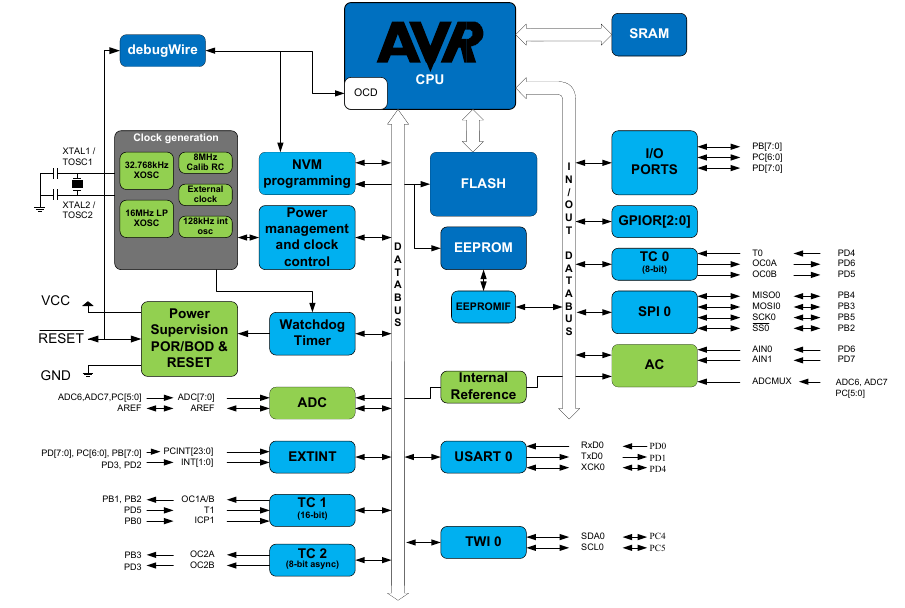
\includegraphics[width=\textwidth]{./Resources/Block_diagram_ATmega328P}
 	\caption{Diagrama de blocos da organiza��o interna do ATmega328P}
 	Fonte: Folha de dados ATmega328P
 	\label{block_diagram_ATmega328P}
 \end{figure}

\section{CPU}

\par A CPU do ATmega328P � apresentada na figura~\ref{block_diagram_cpu}. Ela possui um banco de 32 registradores de 8-bits, com os 6 �ltimos podendo ser utilizados como registradores de 16-bits (chamados de registrador X (R27:R26), Y(R29:R28) e Z(R31:R30)); PC de 14-bits; Registrador de \textit{status} (8-bits) que armazenam as \textit{flags} geradas por cada opera��o aritm�tica/l�gica (zero, \textit{carry}, \textit{overflow}, etc); \textit{Stack Pointer} de 16-bits e demais registradores auxiliares.
 \begin{figure}[h]
	\centering
	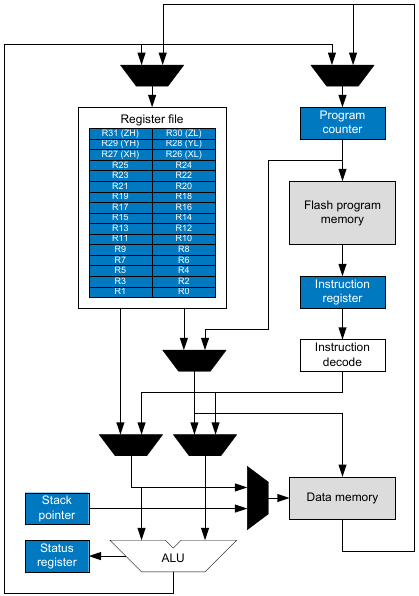
\includegraphics[scale=0.5]{./Resources/Block_diagram_cpu}
	\caption{Diagrama de blocos da organiza��o da CPU}
	Fonte: Folha de dados ATmega328P
	\label{block_diagram_cpu}
\end{figure}

\par A CPU utiliza um \textit{pipeline} de um est�gio o que, junto com a arquitetura Harvard, permite que o sistema atinja uma velocidade m�xima de 1 MIPS/MHz. 
\par Em chamadas de sub-rotinas e interrup��es, a CPU utiliza uma pilha implementada diretamente na mem�ria SDRAM, cujo topo � apontado pelo registrador \textit{Stack Pointer}. Esta estrutura de dados cresce do endere�o mais alto da mem�ria para o endere�o mais baixo, de forma que o \textit{Stack Pointer} deve ser corretamente inicializado para o �ltimo endere�o da mem�ria SDRAM antes de ser utilizado.
\par As interrup��es no ATmega328P s�o organizadas segundo sua prioridade. A tabela~\ref{interruption_vector} mostra o vetor de interrup��es, contendo o endere�o de desvio para cada tipo de interrup��o. Quanto mais baixo o endere�o, maior � a prioridade (o \textit{RESET} � a interrup��o de maior prioridade no sistema).

\begin{table}
	\centering
	\caption{Vetor de interrup��es ATmega328P}
	\label{interruption_vector}
	\begin{tabular}{|c|c|c|}
		\hline
		\textbf{Endere�o de Desvio} & \textbf{Interrup��o} & \textbf{Descri��o}\\ \hline
		0x00 & RESET & Interrup��o de Reset   \\ \hline
		0x02 & INT0  & Interrup��o Externa 0   \\ \hline
		0x04 & INT1 &  Interrup��o Externa 1  \\ \hline
		0x06 & PCINT0 & Interrup��o de mudan�a de estado 0    \\ \hline
		0x08 & PCINT1 & Interrup��o de mudan�a de estado 1   \\ \hline
		0x0A & PCINT2 & Interrup��o de mudan�a de estado 2   \\ \hline
		0x0C & WDT & Estouro do \textit{Watchdog Timer}    \\ \hline
		0x0E & TIMER2\_COMPA  & Compara��o \textit{Timer} 2 canal A    \\ \hline
		0x10 & TIMER2\_COMPB  & Compara��o \textit{Timer} 2 canal B    \\ \hline
		0x12 & TIMER2\_OVF  & Estouro do \textit{Timer} 2    \\ \hline
		0x14 & TIMER1\_CAPT  & Captura de evento \textit{Timer} 1    \\ \hline
		0x16 & TIMER1\_COMPA  & Compara��o \textit{Timer} 1 canal A    \\ \hline
		0x18 & TIMER1\_COMPB  & Compara��o \textit{Timer} 1 canal B    \\ \hline
		0x1A & TIMER1\_OVF  & Estouro do \textit{Timer} 1    \\ \hline
		0x1C & TIMER0\_COMPA  & Compara��o \textit{Timer} 0 canal A    \\ \hline
		0x1E & TIMER0\_COMPB  & Compara��o \textit{Timer} 0 canal B    \\ \hline
		0x20 & TIMER0\_OVF  & Estouro do \textit{Timer} 0    \\ \hline
		0x22 & SPI STC  & Transfer�ncia SPI completa    \\ \hline
		0x24 & USART\_RX  & Recep��o USART completa    \\ \hline
		0x26 & USART\_UDRE  & Registrador de dados vazio (USART)    \\ \hline
		0x28 & USART\_TX  & Transmiss�o USART completa    \\ \hline
		0x2A & ADC  & Convers�o anal�gico-digital completa    \\ \hline
		0x2C & EE READY  & EEPROM pronta    \\ \hline
		0x2E & ANALOG COMP  & Comparador anal�gico    \\ \hline
		0x30 & TWI & Interface serial $I^{2}C$ \\ \hline
		0x32 & SPM READY & Armazenamento na mem�ria de programa \\ \hline
	\end{tabular}
\end{table}

\par Importante resaltar que as interrup��es s�o desabilitadas automaticamente ao iniciar o tratamento de uma rotina de interrup��o (e reabilitadas ao terminar), no entanto, este comportamento pode ser alterado por \textit{software}, reabilitando as interrup��es no come�o da rotina.
\par As interrup��es s�o classificadas em duas classes: as disparadas por envento e as disparadas por uma condi��o. 
\par Quando as interrup��es s�o disparadas por eventos, � habilitada uma \textit{flag} indicando a ocorr�ncia do evento. Se a interrup��o estiver ativada para aquele evento, ela ser� tratada ou enfileirada para execu��o posterior. Ou seja, em interrup��es por evento, os eventos que n�o s�o tratados, s�o lembrados, e ser�o executados em ordem de prioridade assim que poss�vel.
\par Quando o disparo ocorre por uma condi��o, a chamada para a rotina de interrup��o permanece ativa enquanto a condi��o estiver presente. Este tipo de interrup��o n�o necessariamente habilita \textit{flags} de modo que, se a condi��o for removida antes que a CPU possa tratar a interrup��o correspondente, a interrup��o n�o ocorrer�.

\section{Mem�ria de Programa}
\label{sec:memoria_programa}

\par A mem�ria de programa � uma FLASH de 32kB x 8-bits, que est� organizada da forma 16kB x 16-bits pois cada instru��o do microcontrolador � de 16 ou 32-bits. Assim, o registrador PC de 14-bits pode fazer um endere�amento a palavra na mem�ria de programa. 
\par A figura~\ref{program_memory} mostra a organiza��o da mem�ria de programa. Pode-se notar que o \textit{Boot Loader} est� posicionado em uma se��o separada do restante da mem�ria e isso ocorre por quest�es de seguran�a.

 \begin{figure}[h]
	\centering
	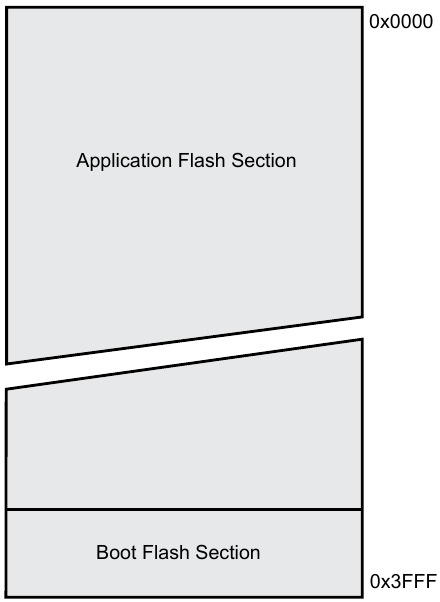
\includegraphics[scale=0.5]{./Resources/program_memory}
	\caption{Mem�ria de programa ATmega328P}
	Fonte: Folha de dados ATmega328P
	\label{program_memory}
\end{figure}

\par As instru��es a serem preenchidas na mem�ria de programa s�o fornecidas pelo arquivo hexadecimal gerado pelo compilador. Este arquivo segue o padr�o Intel e est� disposto conforme mostra a tabela~\ref{tab:intel_hex}~\cite{IntelHex}:

\begin{table}[h]
	\centering
	\caption{Formato dos registros do arquivo hexadecimal no padr�o Intel}
	\label{tab:intel_hex}
	\begin{tabular}{|c|c|c|c|c|c|}
		\hline
		In�cio do registro & Contagem de bytes & Endere�o &  Tipo de registro & Dado & \textit{Checksum} \\ \hline
	\end{tabular}
\end{table}

\begin{itemize}
	\item In�cio do registro: Denotado pelo s�mbolo ":" (1 byte do registro).
	\item Contagem de bytes: Indica a quantidade de bytes a serem lidos no campo de dados (1 byte do registro).
	\item Endere�o: Indica o endere�o de mem�ria no qual deve se iniciar o preenchimento dos dados. Este endere�o pode n�o ser igual ao endere�o f�sico da mem�ria (2 bytes do registro).
	\item Tipo do registro: Indica o que o registro representa (1 byte do registro), podendo ser:
	
	\begin{itemize}
		\item 00: Dado
		\item 01: Fim do arquivo
		\item 02: Segmento estendido de mem�ria. O valor do campo dado � armazenado e o endere�o f�sico de mem�ria dos registros seguintes � calculado como sendo o campo de endere�o somado ao segmento estendido multiplicado por 16.
		\item 03: In�cio do segmento de mem�ria. O valor contido no campo dado � carregado para os registradores CS e IP para os processadores 8086 e 80186
		\item 04: Segmento estendido de mem�ria Linear. O valor do campo dado � armazenado e o endere�o f�sico de mem�ria dos registros seguintes � calculado como sendo o campo de endere�o concatenado ao segmento estendido, sendo este �ltimo a parte mais significativa do endere�o.
		\item 05: In�cio do endere�o linear. Aponta para o endere�o de mem�ria onde o programa deve iniciar a execu��o.
	\end{itemize}

	\item Dado: Cont�m os dados do registro no formato \textit{Little-endian} (primeiro byte � o menos significativo da palavra) (tamanho vari�vel no registro).
	
	\item \textit{Checksum}: Complemento de dois do byte menos significativo da soma de todos os bytes anteriores do registro (1 byte do registro).	
\end{itemize}

\section{Mem�ria de Dados}

\par O ATmega328P possui 2kB de mem�ria de dados SDRAM, al�m do espa�o de dados reservado aos registradores.
\par Apesar dos registradores n�o estarem fisicamente implementados na mem�ria de dados, o microcontrolador faz um mapeamento linear da mem�ria de modo a se obter, na pr�tica, uma mem�ria como mostrado na figura~\ref{data_memory}.

 \begin{figure}[h]
	\centering
	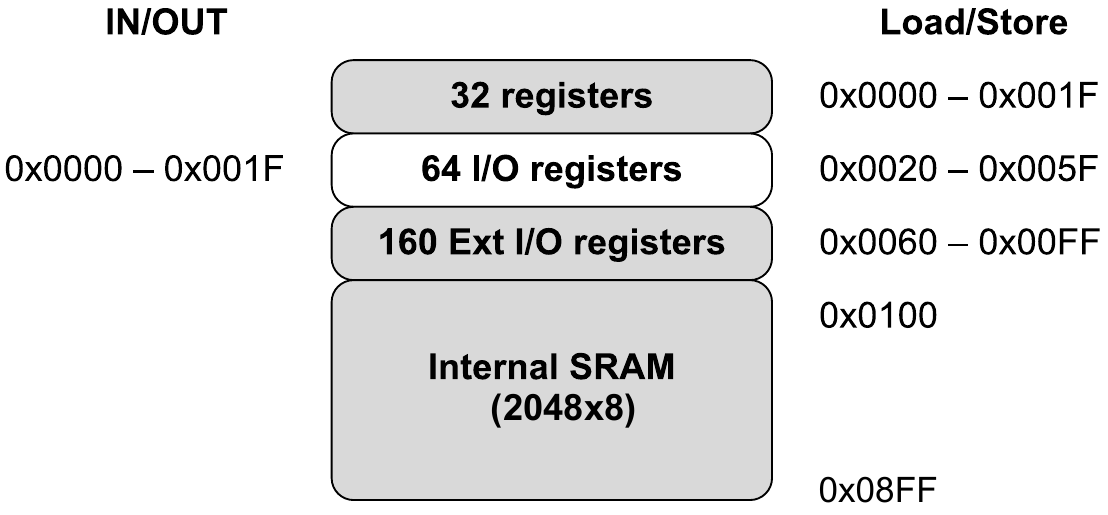
\includegraphics[width=\textwidth]{./Resources/data_memory}
	\caption{Mem�ria de dados ATmega328P}
	Fonte: Folha de dados ATmega328P
	\label{data_memory}
\end{figure}

\par Existem diferentes modos de endere�amento que s�o aplicados � mem�ria de dados. Todo o espa�o de endere�amento suporta qualquer um dos modos listados, s�o eles:

\begin{itemize}
	\item Direto: Acesso direto ao endere�o desejado;
	\item Indireto com deslocamento: Acesso � 63 endere�os deslocados a partir do endere�o base, dado pelo registrador Y ou Z.
	\item Indireto: Acesso ao endere�o dado pelos registradores X, Y ou Z.
	\item Indireto com pr�-decremento: Registradores X, Y ou Z s�o decrementados antes de serem utilizados como ponteiro para endere�amento.
	\item Indireto com p�s-incremento: Registradores X, Y ou Z s�o incrementados depois de serem utilizados como ponteiro para endere�amento.
\end{itemize}


\section{M�dulo de Entrada e Sa�da Digital}
\label{sec:e_s}

\par Como dito anteriormente, o ATmega328P possui 23 pinos program�veis, que podem ser utilizados para entrada ou sa�da de sinal. A figura~\ref{fig:io_module} mostra a organiza��o interna do m�dulo de entrada/sa�da (E/S) do microcontrolador.

 \begin{figure}[h]
	\centering
	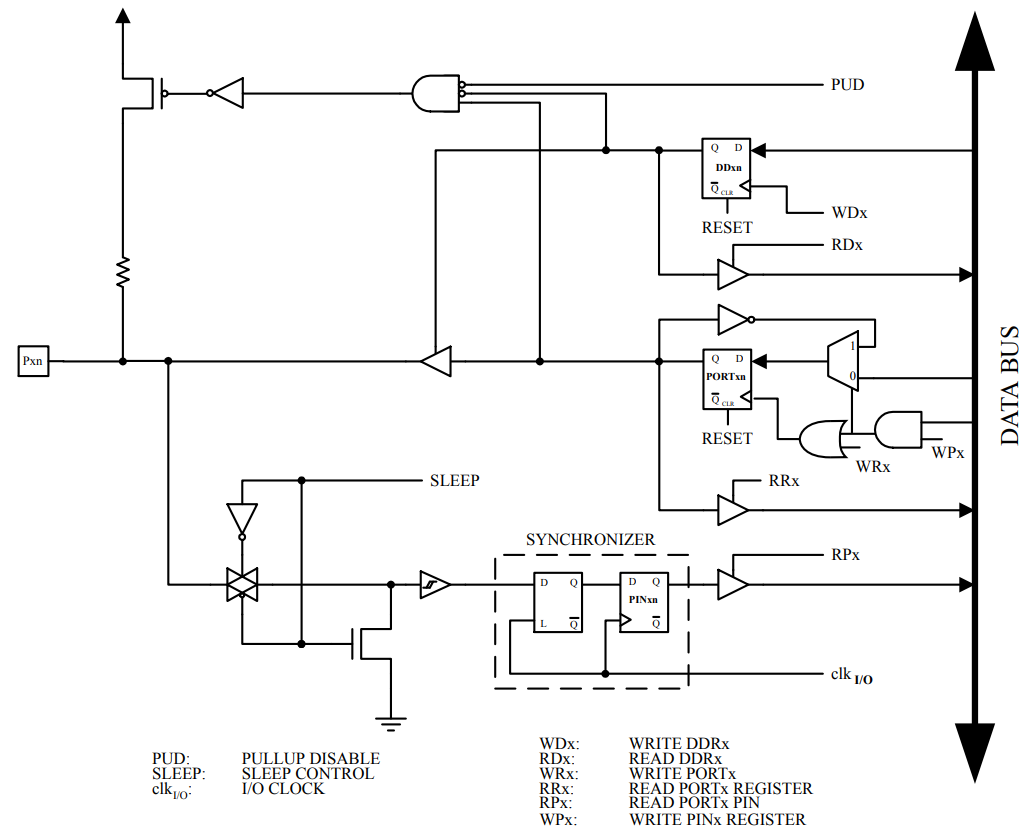
\includegraphics[width=\textwidth]{./Resources/io_module}
	\caption{Organiza��o do m�dulo de Entrada/Sa�da (E/S) do ATmega328P}
	Fonte: Folha de dados ATmega328P
	\label{fig:io_module}
\end{figure}

\par Os pinos podem ser configurados por meio dos registradores DDRxn e PORTxn, onde "x" corresponde � letra do port e "n" corresponde ao n�mero do bit no registrador. O registrador DDRxn � utilizado para configura��o da dire��o do pino (entrada ou sa�da), enquanto o PORTxn configura o estado do pino (n�vel alto ou baixo) se este for um pino de sa�da, caso contr�rio, seu efeito ser� ativar ou desativar o resistor de \textit{pull-up} interno, se este estiver habilitado no registrador MCUCR.
\par Existe ainda o registrador PINxn, que � um registrador apenas de leitura respons�vel por armazenar o valor da entrada do pino. No entanto, � poss�vel escrever um valor "1" neste registrador. O efeito desta escrita ser� a invers�o do valor contido no registrador PORTxn, independente da configura��o do pino como entrada ou sa�da.
\par Al�m de entrada e sa�da digital, alguns pinos possuem fun��es adicionais, tais como entrada anal�gica, sa�da de PWM, etc, que s�o multiplexadas ao funcionamento normal do pino.
\par O m�dulo de E/S pode disparar interrup��es externas (pinos INT) ou interrup��es por mudan�a de valor (pinos PCINT). As interrup��es externas podem ser configuradas para gerar interrup��o por mudan�a de estado, borda de subida/descida ou disparo por n�vel baixo, enquanto as interrup��es por mudan�a de valor n�o s�o configur�veis e apenas respondem � mudan�a de estado na entrada. � interessante notar que as interrup��es por n�vel s�o detectadas de maneira ass�ncrona, podendo ser utilizadas para despertar o sistema se este estiver em determinados modos de hiberna��o.

\section{Temporizadores}
\label{sec:timers}

\par O ATmega328P possui 3 temporizadores internos, chamados \textit{Timer 0},\textit{Timer 1} e \textit{Timer 2}. Os modos de funcionamento dispon�veis para cada temporizador s�o semelhantes, sendo eles: modo normal, modo CTC, \textit{Fast PWM} e PWM com corre��o de fase. As fontes de clock para os temporizadores podem ser externa ou interna. Quanto interna, existe a possibilidade de controle da frequ�ncia por meio de um \textit{prescaler}.
\par O \textit{Timer 1} � um contador de 16-bits, enquanto os \textit{Timers 0} e \textit{2} s�o de 8-bits. O \textit{Timer 2} possui uma fun��o adicional de funcionamento ass�ncrono, podendo assim utilizar uma fonte de clock externa aplicada aos pinos TOSC1 e TOSC2 (os \textit{Timers 0} e \textit{1}, embora tamb�m possam ser acionados por clock externo, a detec��o de borda que � realizada nos pinos T0 e T1 � feita de maneira s�ncrona). Tamb�m por seu funcionamento ass�ncrono, pode ser utilizado para despertar o sistema caso este esteja em determinados modos de hiberna��o. 
\par Os temporizadores podem atuar nos pinos de sa�da OCxA e OCxB, sobrescrevendo a opera��o normal do pino. Para isso, entretanto, � preciso que os pinos sejam configurados como sa�da no registrador DDRxn.
\par As figuras~\ref{fig:timer0_2} e~\ref{fig:timer1} apresentam a organiza��o interna dos \textit{Timers 0/2} e do \textit{Timer 1} respectivamente.

 \begin{figure}[h]
	\centering
	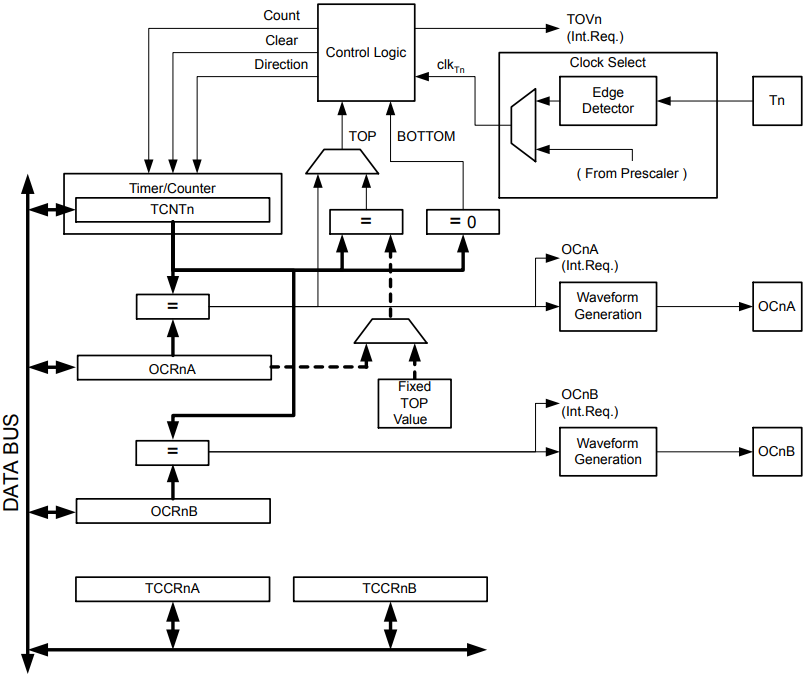
\includegraphics[width=\textwidth]{./Resources/timer0_2}
	\caption{Organiza��o do m�dulo de \textit{Timer 0/2} do ATmega328P}
	Fonte: Folha de dados ATmega328P
	\label{fig:timer0_2}
\end{figure}

 \begin{figure}[]
	\centering
	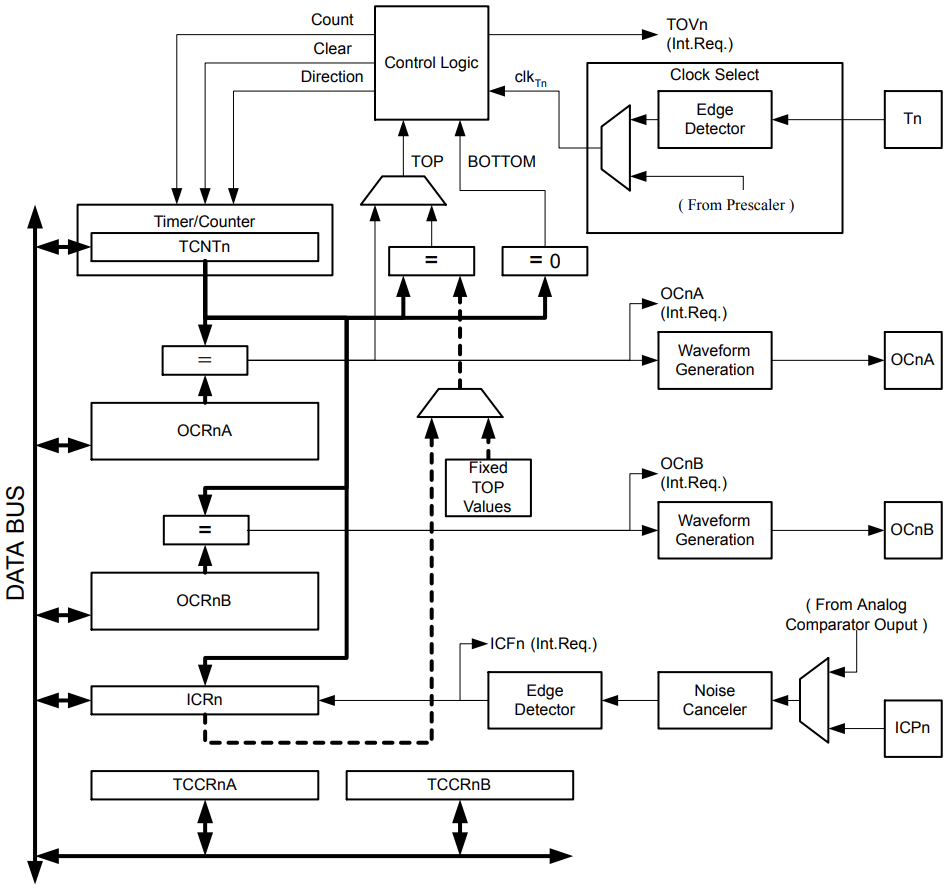
\includegraphics[width=\textwidth]{./Resources/timer1}
	\caption{Organiza��o do m�dulo de \textit{Timer 1} do ATmega328P. Para contar em 16-bits, os registradores TCNTn, ICRn, OCRnA e OCRnB s�o divididos em dois registradores de 8-bits (\textit{Low} e \textit{High}).}
	Fonte: Folha de dados ATmega328P
	\label{fig:timer1}
\end{figure}

\subsection{Modo Normal}

\par No modo normal de opera��o, a contagem � feita continuamente at� atingir o valor m�ximo (0xFF para 8-bits e 0xFFFF para 16-bits), quando ocorre um \textit{overflow} e o sistema reinicia a contagem do zero. O estouro do contador pode ser utilizado para gerar uma interrup��o.
\par Os registradores OCRnA e OCRnB s�o continuamente comparados com o valor de TCNTn (que armazena a contagem) e em caso de \textit{match}, podem gerar interrup��es no sistema e/ou atuar nos pinos OCxA e OCxB, podendo lev�-los � n�vel alto, baixo ou inverter seus valores.

\subsection{Modo CTC}

\par O modo de funcionamento CTC apresenta as mesmas possibilidades do modo normal, no entanto o valor m�ximo de contagem � igual ao valor contido no registrador OCRxA, que pode ser ajustado a qualquer momento (Para o \textit{Timer 1}, existe a op��o de utilizar o registrador ICR1). 
\par No entanto, diferente do modo normal, o rein�cio da contagem n�o pode gerar interrup��o de \textit{overflow}. Isso s� � poss�vel caso OCRxA (ou ICR1) seja igual � 0xFF (8-bits) ou 0xFFFF (16-bits). Neste caso, o modo CTC e o modo normal se comportam de maneiras id�nticas.

\subsection{Modo \textit{Fast PWM}}

\par No modo \textit{fast PWM}, assim como no modo normal, a contagem � feita continuamente do valor mais baixo (0) ao valor mais alto (0xFF para 8-bits ou, no caso do \textit{Timer 1}, este valor pode ser configurado para 0xFF, 0x1FF ou 0x3FF), havendo a possibilidade de altera��o deste valor utilizando o registrador OCRnA (ou ICR1 para o \textit{Timer 1}), como ocorre no modo CTC. Tamb�m como no modo normal, o estouro do contador pode gerar interrup��o de \textit{overflow}.
\par A diferen�a do modo \textit{fast PWM} est� na maneira como um \textit{math} entre TCNTn e OCRnA/OCRnB � tratado. Al�m das possibilidades de disparo de interrup��o, os pinos OCxA/OCxB podem ser configurados para apresentar n�vel baixo em caso de \textit{math} e n�vel alto no estouro do contador (modo de funcionamento n�o-invertido), ou o contr�rio (modo de funcionamento invertido) de modo a gerar uma onda quadrada.

\par Outra caracter�stica do modo \textit{fast PWM} est� na atualiza��o dos valores de OCRnA/OCRnB. Enquanto no modo normal e no modo CTC estes valores s�o atualizados imediatamente, no modo \textit{fast PWM} a atualiza��o dos valores ocorre apenas quando TCNTn atinge o valor m�ximo da contagem. Com isso, evita-se que uma compara��o seja perdida caso o valor de OCRnA/OCRnB seja menor que o valor de TCNTn, o que pode ocorrer nos modos normal e CTC.

\subsection{Modo PWM com Corre��o de Fase}

\par O modo PWM com corre��o de fase faz a contagem progressiva at� o valor m�ximo (fixo ou vari�vel, da mesma forma como ocorre no modo \textit{fast PWM}), seguido de uma contagem regressiva at� o valor m�nimo (0), quando � disparada a condi��o de \textit{overflow}. Esta caracter�stica, faz com que este modo atinga velocidades 2x menor que o modo \textit{fast PWM}.

\par Neste modo de opera��o, os pinos OCxA/OCxB podem ser configurados para apresentar n�vel baixo em caso de \textit{math} com OCRxA/OCRxB (na contagem progressiva) e n�vel alto em caso de \textit{math} (na contagem regressiva), ou o contr�rio, gerando uma onda quadrada. No caso do \textit{Timer 1}, ainda existe a possibilidade de inverter o valor de OC1A em caso de \textit{match}, seja em contagem progressiva ou regressiva.

\par Assim como no modo \textit{fast PWM}, a atualiza��o do valor de OCRxA/OCRxB n�o � instant�nea, ocorrendo apenas no momento em que que a contagem atinge o valor m�ximo. Importante resaltar que, tanto para o modo de corre��o de fase, quanto para o \textit{fast PWM}, o valor de ICR1 � atualizado imediatamente, o que pode ocasionar em uma perda na compara��o com TCNTx caso este registrador estiver sendo usado para definir o topo da contagem.

\subsection{Modo PWM com Corre��o de Fase e Frequ�ncia}

\par Este modo de opera��o est� dispon�vel apenas para o \textit{Timer 1}. Seu funcionamento � id�ntico ao modo de corre��o de fase, a diferen�a est� no momento da atualiza��o dos registradores OCRxA/OCRxB, que n�o ocorre no topo da contagem mas sim ao atingir o valor m�nimo. Com isso, pode-se garantir a simetria dos pulsos gerados.

\subsection{Captura de Eventos}

\par O \textit{Timer 1} apresenta uma funcionalidade extra que � a captura de eventos. Esta funcionalidade permite que o valor da contagem presente em TCNTx seja capturado e salvo no registrador ICR1. 
\par O disparo do evento de captura pode ser dado pela sa�da do comparador anal�gico ou pelo pino ICP1, que pode ser configurado para disparo por borda de subida ou descida.
\par Se o registrador ICR1 n�o estiver sendo utilizado como valor m�ximo do contador, esta � a �nica forma de escrever neste registrador.

\section{Conversor A/D}
\label{sec:conversor_ad}

\par O ATmega328P possui um conversor anal�gico/digital (A/D) com resolu��o de 10-bits e 8 canais de entrada (ADC0-ADC7) multiplexados, al�m de duas entradas fixas (0V e 1,1V) e um sensor de temperatura integrado. A figura~\ref{fig:adc} apresenta a organiza��o interna do conversor A/D.

\par O conversor possui uma entrada de alimenta��o separada que � feita por meio do pino AVcc. Esta entrada pode ser utilizada como tens�o de refer�ncia ($V_{ref}$) para convers�o, ou ainda, podem ser escolhidas outras op��es por meio do registrador ADMUX, tais como a entrada AREF ou refer�ncia interna de 1,1V.

\par Por ser um conversor de 10-bits, s�o necess�rios 2 registradores para armazenar o resultado da convers�o, s�o eles o ADCL e o ADCH. O resultado da convers�o � alinhado � esquerda por padr�o, no entanto esta op��o pode ser alterada para alinhamento � direita por meio do registrador ADMUX. A figura~\ref{fig:alinhamento} mostra como o resultado � armazenado nos registradores ADCL e ADCH para cada modo.

\begin{figure}[h]
	\centering
	\begin{subfigure}{0.75\textwidth}
		\centering
		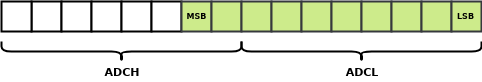
\includegraphics[width = \textwidth]{./Resources/adc_left_align}
		\caption{Alinhamento � esquerda}
	\end{subfigure}
	
	%Line Break
	
	\begin{subfigure}{0.75\textwidth}
		\centering
		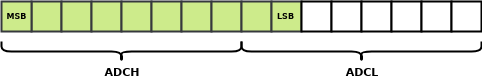
\includegraphics[width = \textwidth]{./Resources/adc_right_align}
		\caption{Alinhamento � direita}
	\end{subfigure}
	\caption{Alinhamento do resultado nos registradores ADCH e ADCL}
	Fonte: Autor.
	\label{fig:alinhamento}
\end{figure}

 \begin{figure}
	\centering
	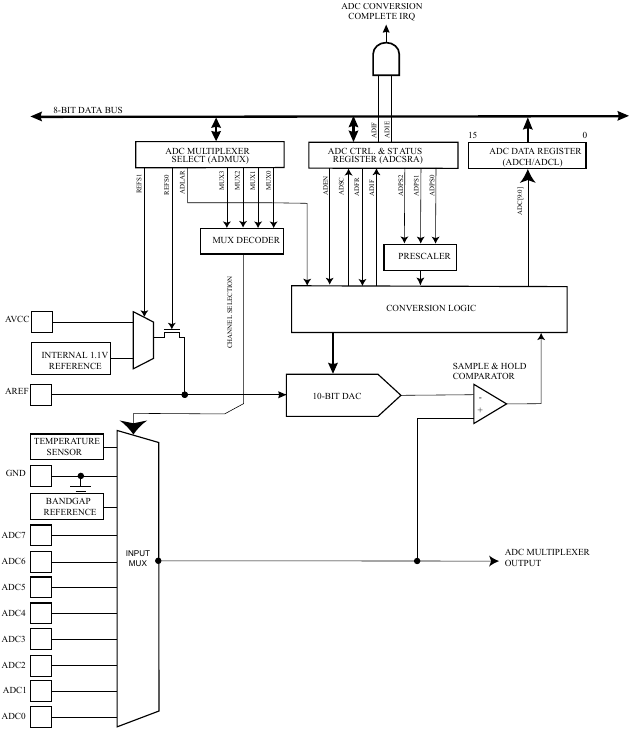
\includegraphics[width=\textwidth]{./Resources/adc}
	\caption{Organiza��o do conversor A/D}
	Fonte: Folha de dados ATmega328P
	\label{fig:adc}
\end{figure}

\par Por seguran�a, uma leitura no registrador ADCL bloqueia a permiss�o de escrita nos registradores ADCL e ADCH, garantindo assim que o dado lido � referente � mesma convers�o (o acesso � liberado novamente ao realizar uma leitura em ADCH). Caso o resultado esteja alinhado � direita, pode-se obter um valor convertido de 8-bits apenas lendo o registrador ADCH.

\par Para iniciar uma convers�o � necess�rio colocar em n�vel alto os bits ADEN (habilita o conversor) e ADSC. A convers�o � ent�o inicializada e ADSC permanece em n�vel alto durante todo o tempo de convers�o. Ao final, o bit ADSC � resetado por \textit{hardware} e a \textit{flag} ADIF � setada, podendo gerar uma interrup��o se esta estiver configurada. O resultado de uma convers�o � dada pela equa��o~\ref{eq:adc_result}.

\begin{equation}
	ADC = \frac{V_{in} * 1024}{V_{ref}}
	\label{eq:adc_result}
\end{equation}

\par Valores de entrada superiores � $V_{ref}$ ter�o valores convertidos pr�ximos � 0x3FF (m�ximo valor para 10-bits).

\par � poss�vel configurar um evento para o disparo do conversor A/D ou utiliz�-lo no modo \textit{Free Run}, em que o disparo do conversor � feita pela pr�pria \textit{flag} do conversor (ADIF), fazendo com que uma nova convers�o comece imediatamente ap�s a outra. Para utilizar este modo, a \textit{flag} ADIF precisa ser limpa a cada convers�o, o que � feito automaticamente se for utilizada interrup��o. A tabela~\ref{tab:disparo_adc} apresenta todas as possibilidades de disparo do conversor A/D.

\begin{table}[h]
	\centering
	\caption{Modos de disparo do conversor A/D}
	\label{tab:disparo_adc}
	\begin{tabular}{|c|c|}
		\hline
		ADTS[2:0] & Disparo \\ \hline
		000& Modo \textit{Free Run}  \\ \hline
		001& Sa�da do comparador anal�gico \\ \hline
		010& Interrup��o externa 0 \\ \hline
		011& \textit{Math} A \textit{Timer} 0 \\ \hline
		100& \textit{Overflow Timer 0} \\ \hline
		101& \textit{Math} B \textit{Timer} 1 \\ \hline
		110& \textit{Overflow Timer 1} \\ \hline
		111& Captura de evento \textit{Timer} 1 \\ \hline
	\end{tabular}
\end{table}

\par Um recurso extra oferecido pelo microcontrolador � o sensor de temperatura integrado. Este sensor � capaz de realizar medi��es entre -45\textdegree C e 85\textdegree C, com precis�o de $\pm$10\textdegree C. 
\par Para utilizar este sensor, � preciso configurar o $V_{ref}$ para a entrada interna de 1,1V. A temperatura (em \textdegree C) � dada pela equa��o~\ref{eq:adc_temperatura}.

\begin{equation}
	T = \frac{[ADCH << 8 | ADCL] - T_{OS}}{k}
	\label{eq:adc_temperatura}
\end{equation}

\par Onde $T_{OS}$ � um valor inserido na EEPROM de cada componente como parte dos testes em produ��o e k � um valor a ser determinado na calibra��o. (Na pr�tica, utiliza-se $T_{OS}$ = 324,31 e k = 1,22~\cite{Sensor_Temperatura})

\section{USART}
\label{sec:usart}

\par Um dos m�dulos que permitem que o ATmega328P realize comunica��o serial � a USART. Esta possui m�ltiplos modos de opera��o, suportando comunica��o \textit{full duplex}, opera��o s�ncrona e ass�ncrona, detec��o de erros em \textit{frames}, modo de comunica��o com multiprocessadores, etc., al�m de poder ser utilizada para comunica��o SPI (como Mestre). A figura~\ref{fig:usart} apresenta a organiza��o interna deste m�dulo no microcontrolador.

 \begin{figure}
	\centering
	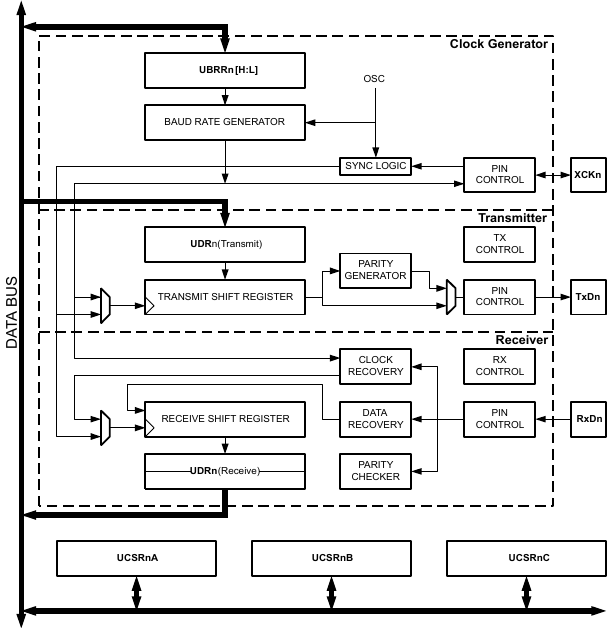
\includegraphics[width=\textwidth]{./Resources/usart}
	\caption{Organiza��o da USART}
	Fonte: Folha de dados ATmega328P
	\label{fig:usart}
\end{figure}

\par O protocolo de comunica��o da USART utiliza \textit{frames} que podem ter 5,6,7,8 ou 9 bits, com 1 ou 2 bits de parada, al�m da possibilidade de adi��o de bits de paridade par ou �mpar. A transmiss�o de um \textit{frame} se inicia com o bit de \textit{START}, fazendo a mudan�a do estado da linha alto (\textit{IDLE}) para o n�vel baixo, indicando que uma comunica��o deve ser iniciada. Os bits do \textit{frame} s�o ent�o transmitidos um a um, come�ando pelo bit menos significativo e terminando com o bit de paridade (se houver). Por fim, s�o enviados os bits de parada (1 ou 2, conforme configurado), indicando o fim do \textit{frame}. Este procedimento est� ilustrado na figura~\ref{fig:frame_usart}.

 \begin{figure}
	\centering
	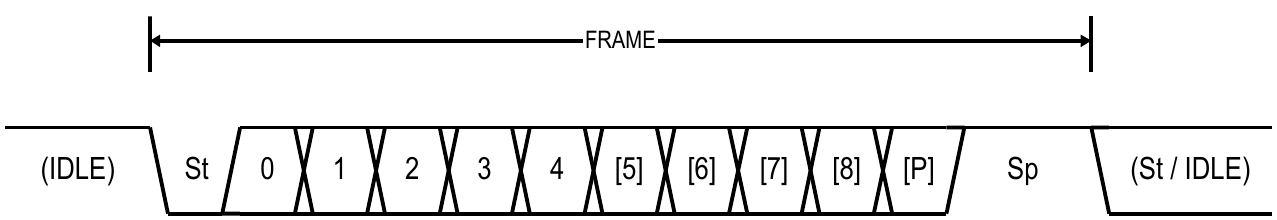
\includegraphics[width=\textwidth]{./Resources/frame_usart}
	\caption{Formato de um \textit{frame} transmitido pela USART.}
	Fonte: Folha de dados ATmega328P
	\label{fig:frame_usart}
\end{figure}
\chapter{Desenvolvimento do Projeto}
\label{Material}


\par Neste cap�tulo ser�o detalhadas as etapas de desenvolvimento do projeto, bem como as ferramentas utilizadas.
% % % % % % % % % % % % % % % % % % % % % % % % % % % % % % % % % % % % % % % % % % % % % % % % % % %
\section{Material}

\par Para a execu��o do projeto foram necess�rias diversas ferramentas para projetar, desenvolver e testar o sistema. A seguir s�o listados todos os materiais utilizados ao longo do projeto.

\begin{itemize}
\item Para o desenho de diagramas de classe e mapas mentais na fase de projeto, foram utilizadas as ferramentas \href{http://dia-installer.de/}{\textit{Dia}} e \href{https://www.draw.io/}{\textit{Draw.io}}.

\item Foi utilizado o m�todo �gil \textit{Scrum} para a constru��o do sistema. A plataforma \href{https://taiga.io/}{\textit{Taiga}} foi utilizada para organiza��o e planejamento dos \textit{Sprints}.

\item Para controle de vers�o foi utilizado o \href{https://git-scm.com/}{\textit{Git}} sincronizado � um reposit�rio \textit{on-line} no \href{https://github.com/}{\textit{Github}}.

\item Para documenta��o do projeto, foi utilizada uma p�gina do \href{www.gitbook.com}{\textit{Gitbook}}.

\item Para o realizar modifica��es no c�digo da IDE do Arduino, foi utilizado o \href{https://www.jetbrains.com/idea/}{\textit{InteliJ IDEA}} para escrever o c�digo e o \href{https://ant.apache.org/}{\textit{Apache Ant}} para a compila��o. Tamb�m foi utilizado o \href{https://inkscape.org/pt-br/}{\textit{Inkscape}} para a altera��o no \textit{design} (inser��o do bot�o "Android").

\item Para o desenvolvimento \textit{mobile}, foi utilizada a IDE \href{https://developer.android.com/studio/}{\textit{Android Studio}}.

\item Para criar testes de unidade, foi utilizado o \href{https://junit.org/junit4/}{\textit{JUnit4}} em conjunto com o \href{https://github.com/powermock/powermock}{\textit{PowerMock}} (ambos utilizados como \textit{plugin} do \href{https://gradle.org/}{\textit{Gradle}}).

\item O \href{https://www.sonarqube.org/}{\textit{SonarQube}} foi utilizado para fazer a analise est�tica do c�digo do simulador. Em conjunto, foi utilizado o \href{https://www.eclemma.org/jacoco/}{\textit{JaCoCo}} para obter medidas de cobertura de c�digo.

\item Para montar c�digos \textit{Assembly} escritos para o ATmega328P, foi utilizado o \href{http://avra.sourceforge.net/}{\textit{AVRA}}.

\item Em termos de hardware, foi utilizado um Arduino UNO R3 para comparar os resultados obtidos pelo aplicativo com o sistema real, principalmente compara��es feitas em medidas de frequ�ncia, no qual se fez uso tamb�m de um oscilosc�pio InfiniiVision DSOX2002A, da Keysight.
\end{itemize}


% % % % % % % % % % % % % % % % % % % % % % % % % % % % % % % % % % % % % % % % % % % % % % % % % % %
\newpage
\section{M�todo}

\subsection{Desenvolvimento na IDE do Arduino}

\par A primeira parte do desenvolvimento ocorreu na IDE do Arduino. N�o houve muito desenvolvimento nela al�m da cria��o do bot�o "Android", cuja fun��o � compilar o c�digo e transferi-lo para o aparelho Android conectado ao computador, da mesma forma que o bot�o "\textit{Upload}" faz com a placa de Arduino. A figura~\ref{fig:diagrama_classes_usb} apresenta o diagrama de classes do c�digo desenvolvido nesta etapa.

 \begin{figure}[h]
	\centering
	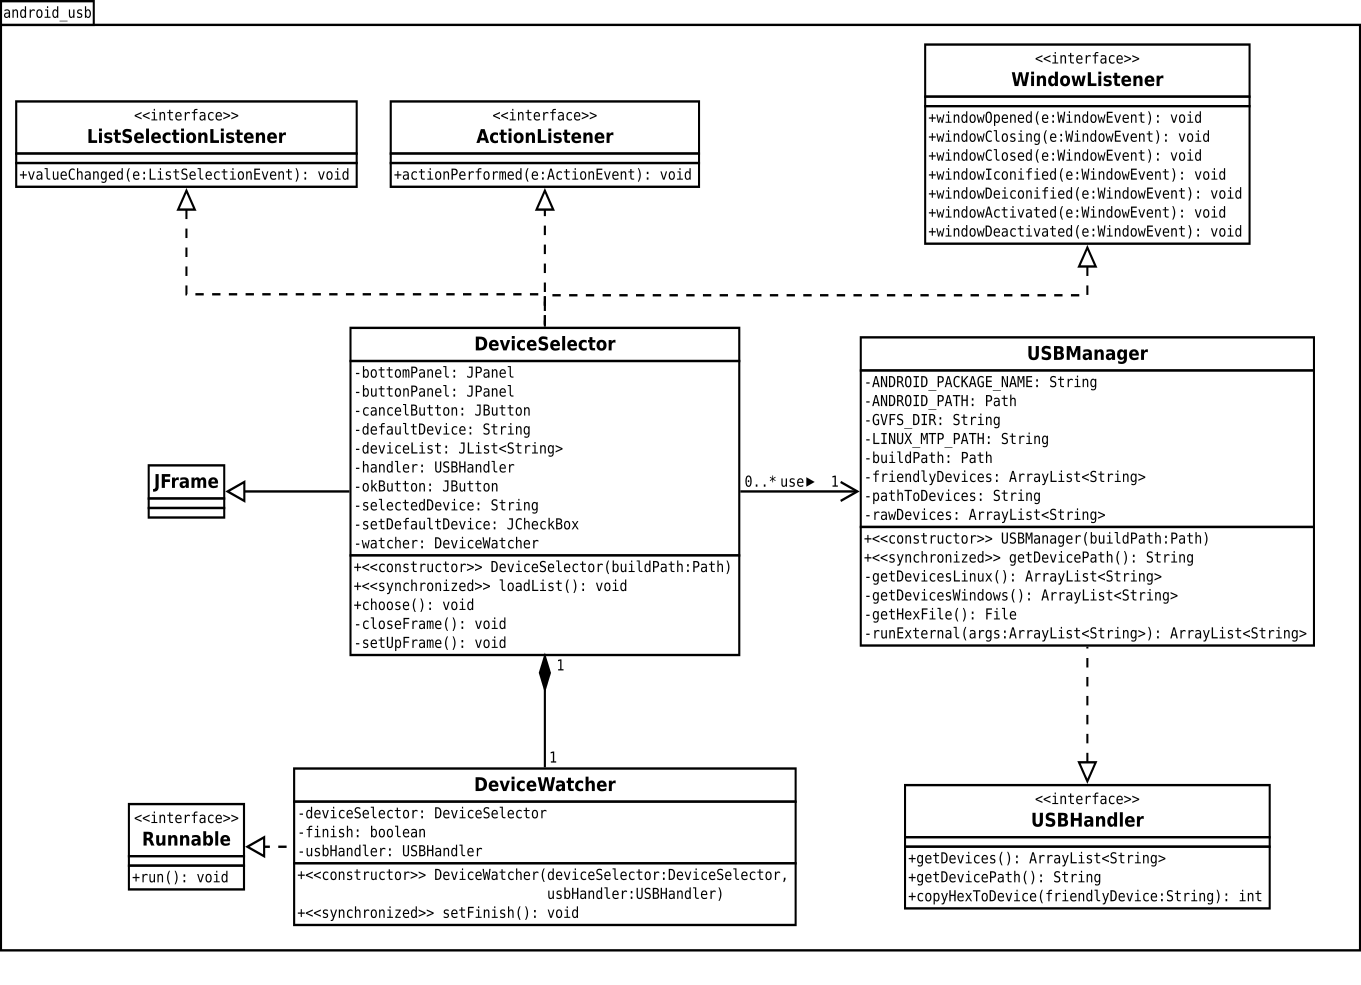
\includegraphics[width=\textwidth]{./Resources/usb_class_diagram}
	\caption{Diagrama de classes das modifica��es realizadas na IDE do Arduino}
	Fonte: Autor
	\label{fig:diagrama_classes_usb}
\end{figure}

\par A classe \textit{DeviceSelector} � a entrada do sistema. Ela recebe como argumento o local onde o hexadecimal � gerado (que pode ser obtido por meio do m�todo \textit{getBuildPath} da classe \textit{Sketch} j� existente no projeto do Arduino) e cria a janela para selecionar o dispositivo. Todos os aparelhos Android montados no sistema s�o exibidos em uma lista em caso de sucesso na compila��o. Em conjunto, atua a classe \textit{DeviceWatcher}, que � uma \textit{thread} que fica a procura de novos dispositivos. Desta forma, caso algum aparelho seja conectado ap�s a exibi��o da janela de sele��o, a lista de dispositivos � atualizada automaticamente.

\par J� a classe \textit{USBManager} cuida de toda a comunica��o com o sistema e o dispositivo Android, al�m de fazer a identifica��o dos dispositivos conectados e retornar ao seletor um \textit{friendly name} para que o usu�rio possa reconhecer seu dispositivo facilmente. Ao pressionar o bot�o "Ok" do seletor de dispositivos, o m�todo \textit{copyHexToDevice} � chamado para copiar o arquivo compilado para o dispositivo Android.

\par No Linux, todos os dispositivos MTP s�o montados por meio do \textit{GNOME Virtual file system} (GVfs). Utilizando a vari�vel de ambiente \textit{\$XDG\_RUNTIME\_DIR} � pos�vel acessar o dispositivo como uma pasta no sistema de arquivos. Desta forma, o arquivo .hex � copiado para o local \url{XDG\_RUNTIME\_DIR/gvfs/<Dispositivo>/DCIM/SOFIA} e tem o nome gen�rico de \textit{code.hex}, tornando o c�digo dispon�vel para o simulador.

\par No Windows, dispositivos MTP s�o tratados de forma diferente, n�o sendo montados diretamente no sistema de arquivos, tornando o acesso bastante trabalhoso. Por este motivo, nesta primeira vers�o do sistema, n�o foi implementado um m�todo autom�tico para copiar o arquivo .hex para o dispositivo Android no Windows.

\par A classe \textit{USBManager} utiliza alguns comandos externos do sistema, tais como \textit{lsusb}, \textit{gio copy} e \textit{gvfs-copy}. O primeiro comando � necess�rio apenas para retornar um nome mais leg�vel do dispositivo para o usu�rio (\textit{friendly name}), mas caso este n�o seja encontrado o sistema ainda ser� capaz de funcionar. J� o segundo e o terceiro comando s�o utilizados para transferir o arquivo para o dispositivo m�vel, sendo executados na ordem: primeiro o \textit{gio copy}, seguido do \textit{gvfs-copy} em caso de falha (\textit{gvfs-copy} � um comando antigo, mas foi adicionado para compatibilidade). Se o usu�rio n�o tiver pelo menos um destes comandos dispon�veis no computador, o sistema informar� falha ao copiar o arquivo. (Estes comandos fazem parte do pacote b�sico de instala��o das principais distribui��es Linux.)

%\par O bot�o "Android" foi posicionado junto aos demais bot�es j� existentes na IDE, na parte superior esquerda, conforme mostra a figura~\ref{fig:botao_android}.

% \begin{figure}[h]
%	\centering
%	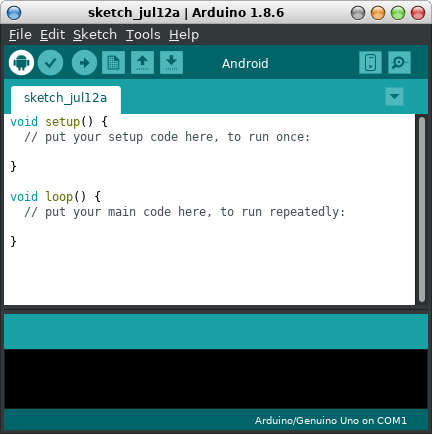
\includegraphics[width=0.5\textwidth]{./Resources/android_button}
%	\caption{Localiza��o do bot�o "Android" (primeiro da esquerda para a direita) na IDE.} 
%	Fonte: Autor
%	\label{fig:botao_android}
%\end{figure}


\subsection{Desenvolvimento Android}

\subsubsection{Arquitetura}

A segunda parte do desenvolvimento foi a cria��o do aplicativo para fazer a simula��o do c�digo. A figura~\ref{fig:arquitetura_simulador} apresenta um diagrama simplificado da arquitetura do simulador.

 \begin{figure}[h]
	\centering
	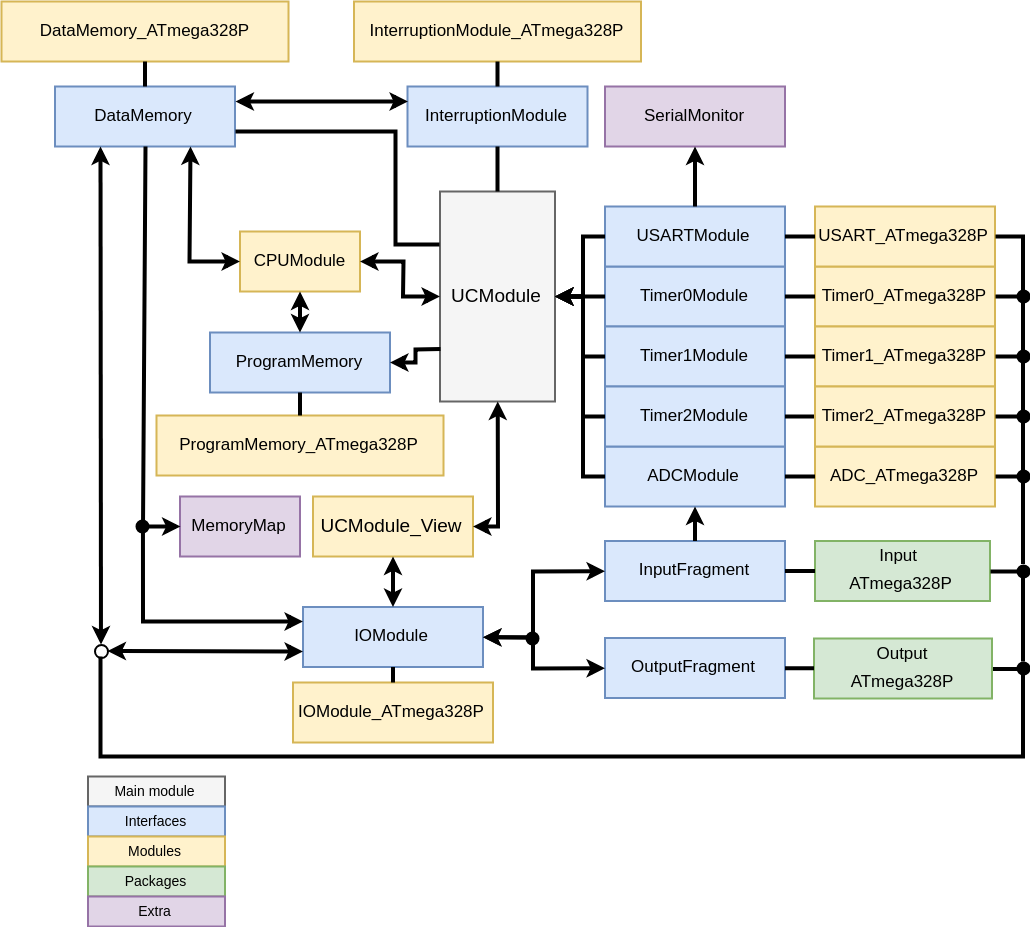
\includegraphics[width=\textwidth]{./Resources/ArduinoSimulator_arquitetura}
	\caption{Arquitetura do simulador} 
	Fonte: Autor
	\label{fig:arquitetura_simulador}
\end{figure}

\subsubsection{M�dulo principal}

\par Tudo tem in�cio na classe \textit{UCModule}, que constitui o m�dulo principal do sistema. Esta classe � respons�vel por inicializar todos os demais m�dulos e fazer a sincroniza��o entre eles, al�m de fornecer servi�os para estes m�dulos no que diz respeito �s caracter�sticas do sistema simulado, como a quantidade de pinos, tens�o de alimenta��o, etc. Esta classe possui uma extens�o que � a classe \textit{UCModule\_View}. Ela � respons�vel por toda a manipula��o das telas e recursos visuais do aplicativo, al�m de fornecer \textit{feedback} � \textit{UCModule} quanto �s a��es dos bot�es (como bot�o \textit{Reset}) e fazer a contagem do tempo simulado. � na \textit{UCModule\_View} que os m�dulos de entrada e sa�da s�o inicializados.

\par Outra tarefa da \textit{UCModule} � atuar como escalonador. Todos os m�dulos do sistema (CPU, conversor A/D, temporizadores, USART) al�m do m�dulo de visualiza��o (\textit{UCModule\_View}) s�o executados um a um, em uma fila circular, sendo calculado um ciclo de clock a cada itera��o. A velocidade de execu��o deste \textit{loop} n�o foi limitada de nenhuma forma para maximizar a velocidade de simula��o. Ao mesmo tempo, essa abordagem faz com que o simulador sofra varia��es de velocidade em fun��o da carga no sistema Android.

\par Ainda quanto � sincronia dos m�dulos, buscou-se preservar o n�mero correto de ciclos de clock que cada instru��o da CPU leva para executar, bem como chamadas para rotinas de interrup��o e \textit{prescalers} dos temporizadores. A exce��o fica apenas para o conversor A/D, cujo tempo de convers�o � de apenas 1 ciclo de clock (originalmente, o Arduino leva cerca de 13 ciclos) e os \textit{prescalers} foram desabilitados. Essa mudan�a se justifica por n�o afetar de maneira significativa o realismo da simula��o, ao mesmo tempo que proporciona um ganho de performance, tornando o sistema mais agrad�vel ao usu�rio.

\subsubsection{CPU}

\par O pr�ximo m�dulo, a CPU (\textit{CPUModule}), � respons�vel pela execu��o das instru��es contidas na mem�ria de programa. Ao final de cada instru��o, � feita a verifica��o por interrup��es, que s�o executadas em ordem de prioridade conforme apresentado na tabela~\ref{interruption_vector}. Todas as instru��es do microcontrolador ATmega328P foram implementadas, com exce��o das instru��es \textit{BREAK}, \textit{SLEEP} e \textit{WDR}.

\par A arquitetura trabalhada n�o fornece instru��es com campos fixos para \textit{opcode}, operadores, etc., o que dificulta a decodifica��o das instru��es. Para que a legibilidade do c�digo n�o fosse prejudicada com uma s�rie de condicionais aninhadas, a estrat�gia adotada para a decodifica��o foi a utiliza��o de um banco de dados com as instru��es pr�-decodificadas. Desta forma, foi criado um banco de dados com $2^{16}$ posi��es (tamanho da instru��o) e para cada posi��o foi inserido um identificador (ID) da instru��o referente �quela posi��o em bin�rio. Com isso, ao ler uma instru��o da mem�ria de programa, a CPU simplesmente acessa um vetor na posi��o da instru��o lida e recupera a instru��o a ser executada (o banco de dados � carregado para a mem�ria durante a exibi��o do \textit{Splash Screen} ao iniciar o aplicativo). 
\par Apesar do gasto de mem�ria (o tamanho deste banco de dados em mem�ria � de 128kB), esta solu��o torna o c�digo muito mais leg�vel e possivelmente mais r�pido.

\subsubsection{Mem�ria de Programa} 

\par A mem�ria de programa (\textit{ProgramMemory}) � respons�vel por armazenar o c�digo a ser executado pela CPU. O c�digo � lido de um arquivo hexadecimal no formato \textit{Intel HEX} e formatado em um \textit{array} de \textit{bytes}. � tamb�m fun��o da mem�ria de programa verificar continuamente o arquivo hexadecimal e enviar uma mensagem de \textit{Reset} para o m�dulo principal em caso de altera��es.

\par Como dito na se��o~\ref{sec:memoria_programa}, a mem�ria de programa do ATmega328P � organizada em 16kB x 16-bits. No entanto, no simulador, preferiu-se a organiza��o 32kB x 8-bits. Desta forma, a estrutura de dados para armazenar o programa � mais simples (um vetor de \textit{bytes}), al�m de facilitar a implementa��o da instru��o LPM, que realiza a leitura de um \textit{byte} da mem�ria de programa.

\par Cada vez que uma instru��o � lida da mem�ria pela CPU, dois \textit{bytes} s�o lidos e concatenados. O valor do PC continua se referindo ao valor da pr�xima instru��o enquanto que o endere�o dos \textit{bytes} desta instru��o s�o calculados no m�todo \textit{loadInstruction}.

\subsubsection{Mem�ria de Dados} 

\par A mem�ria de dados (\textit{DataMemory}) � o m�dulo respons�vel por armazenar todas as informa��es dos registradores e da mem�ria SDRAM externa. Trata-se de uma classe cujos m�todos de leitura e escrita est�o sincronizados para evitar conflitos. Al�m disso, a mem�ria de dados notifica a classe \textit{IOModule} em caso de altera��o nos registradores de E/S (PINx, PORTx e DDRx).

\par Alguns registradores s�o tratados de maneira diferentes no ATmega328P. Pode-se citar, por exemplo, o registrador PINx. Este, como explicado na se��o~\ref{sec:e_s}, apesar de ser um registrador de leitura, permite tamb�m a escrita de um valor. Esta escrita, no entanto, n�o altera o valor do PINx, mas sim, o valor do PORTx. Estes casos foram todos tratados na mem�ria de dados, nos m�todos de escrita \textit{writeByte} e \textit{writeBit}. Assim, ao escrever um valor na mem�ria, o endere�o � verificado e se um caso especial for detectado, a opera��o realizada ser� diferente de uma simples escrita.
\par Tamb�m foram escritos m�todos especiais para a manipula��o dos registradores que s�o atualizados apenas por \textit{hardware} (como o PINx), bem como para a manipula��o das \textit{flags} de interrup��o.

\par A mem�ria de dados tamb�m fornece informa��es para o mapa de mem�ria quando este � aberto pelo usu�rio. Por realizar mais opera��es de leitura e principalmente devido a maior atualiza��o da tela, a velocidade de simula��o diminui este recurso est� ativo, ficando mais lento quanto mais din�mica for a por��o vis�vel na tela.

\subsubsection{M�dulo de Interrup��o}

\par Foi desenvolvido um m�dulo de interrup��o (\textit{InterruptionModule}) cuja fun��o � verificar e organizar todos os eventos de interrup��o que podem ser gerados. Este m�dulo recebe requisi��es dos m�dulos de \textit{Timer}, E/S, conversor A/D e USART, organizando-as em ordem de prioridade. No caso do m�dulo de E/S, � feita ainda a verifica��o se houve ou n�o uma interrup��o, por meio de detectores de borda, detec��o de n�vel baixo, etc. 
\par Este m�dulo tamb�m � respons�vel por armazenar os endere�os de desvio das interrup��es e fornecer � CPU para a execu��o das rotinas de interrup��o. 
\par Todas as classes do projeto podem acessar o m�dulo de interrup��o estaticamente, por meio da classe \textit{UCModule}.

\subsubsection{M�dulo de E/S} 

\par Seguindo para o m�dulo de entrada e sa�da, este � dividido em duas partes, cada uma tratando exclusivamente entrada ou sa�da. A parte de tratamento de entrada � respons�vel pelo gerenciamento de cada elemento gr�fico de entrada, bem como o tratamento de suas a��es, enquanto que o pacote de sa�da faz o mesmo para os elementos gr�ficos de sa�da. A classe \textit{IOModule} fica acima destas duas, fazendo a integra��o para que a classe \textit{UCModule\_View} possa exibir corretamente os elementos de interface com o usu�rio.

\par N�o foi imposta nenhuma restri��o quanto � liga��o de entradas e sa�das no simulador. Isso significa que o usu�rio pode conectar m�ltiplas entradas/sa�das no mesmo pino, conectar uma entrada anal�gica em um pino digital (neste caso, ser�o adotados os valores de tens�o da folha de dados para definir n�vel alto, baixo ou indefinido), conectar entradas digitais em pinos anal�gicos, etc. Um mecanismo de detec��o de curto-circuito (entre entrada e sa�da, tamb�m entre entradas) atua toda vez que uma entrada ou sa�da � alterada, parando o sistema se alguma condi��o indevida for detectada. 

\par Foram definidos 3 n�veis l�gicos no sistema: alto, baixo e alta imped�ncia. O n�vel de alta imped�ncia � visto apenas na sa�da. Na entrada, existe ainda um estado indefinido, que envia um valor aleat�rio para a entrada, ou seja, pode ser interpretado como n�vel alto ou baixo (exceto se o resistor de \textit{pull-up} interno estiver habilitado).

\subsubsection{Temporizadores} 

\par Foram implementados os 3 temporizadores (\textit{TimerxModule}) presentes no ATmega328P. Eles fornecem todos os modos de funcionamento dos apresentados na se��o~\ref{sec:timers}, com exce��o do funcionamento ass�ncrono para o \textit{Timer} 2.

\par Como mostrado no cap�tulo~\ref{EmbasamentoTeorico}, alguns registradores, tais como a pilha, registradores do \textit{Timer} 1, etc., trabalham em pares (\textit{LOW} e \textit{HIGH}). Em especial, o \textit{Timer} 1 usa um registrador tempor�rio para que a leitura/escrita nos registradores ocorra de maneira sincronizada, ou seja, ao ler um valor de contagem do registrador \textit{LOW}, o registrador \textit{HIGH} � salvo imediatamente para que a leitura seja referente ao mesmo instante de tempo. Da mesma forma, a escrita em um registrador \textit{HIGH} � armazenada em um registrador tempor�rio e s� � realizada de fato quando ocorrer uma escrita no registrador \textit{LOW}, fazendo a escrita simult�nea das duas partes.

\par Este mecanismo de registrador tempor�rio s� foi utilizado para escritas da CPU. No m�dulo de \textit{Timer} 1, a escrita nos registradores de 16-bits ocorre por meio de um m�todo especial na mem�ria de dados, que faz a escrita das duas partes simultaneamente.

\subsubsection{Conversor A/D} 

\par O conversor A/D (\textit{ADCModule}), assim como os Temporizadores, apresenta todos os m�dulos de funcionamento descritos na se��o~\ref{sec:conversor_ad}, com exce��o do sensor de temperatura e do disparo pela sa�da do comparador anal�gico (j� que este m�dulo n�o foi implementado). 

\par Em termos de implementa��o, este � o m�dulo menos fiel ao sistema f�sico original, principalmente em se tratando dos tempos de convers�o. No entanto, isso n�o reflete em uma simula��o incorreta do m�dulo.

\subsubsection{USART}

\par Por fim, a USART (\textit{USARTModule}), apesar de possuir diversos modos de opera��o no sistema f�sico original, possui apenas um modo de opera��o no simulador: \textit{frames} de 8 bits, sem paridade e um bit de parada. Esta configura��o foi escolhida por ser a inicializa��o padr�o da fun��o \textit{Serial.begin()} do Arduino (embora outras configura��es tamb�m sejam poss�veis).

\par Este m�dulo se comunica com um monitor serial que foi integrado ao sistema e ocupa o mesmo espa�o reservado aos pinos de sa�da. Uma caracter�stica deste m�dulo � que a configura��o de velocidade (\textit{BAUD rate}) n�o importa para o funcionamento do m�dulo, ou seja, o comportamento do sistema ser� o mesmo para qualquer velocidade de comunica��o.

\hfil

\par Voltando na figura~\ref{fig:arquitetura_simulador}, pode-se observar que as comunica��es ocorrem sempre por meio de interfaces (exceto para envio de dados, que precisam partir dos m�dulos). Este \textit{design} isola toda a parte de controle do funcionamento dos m�dulos espec�ficos do ATmega328P, o que facilita a expans�o do sistema j� que, para suportar uma nova plataforma, basta escrever novos m�dulos de \textit{Timer}, conversor A/D, etc., que implementem as mesmas interfaces. As �nicas classes que s�o acessados diretamente s�o a \textit{UCModule\_View} (que � pr�pria do aplicativo) e a \textit{CPUModule} (que � pr�pria da arquitetura AVR).

\chapter{Resultados e Discuss�es}
\label{Resultados}

\par Nesta se��o, ser�o apresentados os resultados obtidos com as modifica��es da IDE do Arduino e com o simulador para Android, bem como algumas m�tricas de \textit{software} obtidas para o simulador e algumas compara��es feitas com aplicativos semelhantes ao desenvolvido neste trabalho.

\section{Arduino IDE}

\par A figura~\ref{fig:ide_modificada} mostra o como ficou a IDE do Arduino ap�s a introdu��o do bot�o "Android".

 \begin{figure}[h]
	\centering
	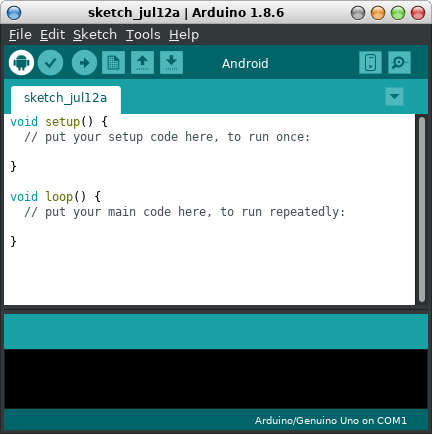
\includegraphics[width=0.6\textwidth]{./Resources/android_button}
	\caption{Localiza��o do bot�o "Android" (Selecionado) na IDE} 
	Fonte: Autor
	\label{fig:ide_modificada}
\end{figure}

\par Ao pressionar o bot�o "Android", o processo de compila��o se inicia e, em caso de sucesso, � exibida a janela para a sele��o do dispositivo Android conectado ao PC, como mostrado na figura~\ref{fig:selecionar_dispositivo}.

\begin{figure}[h]
	\centering
	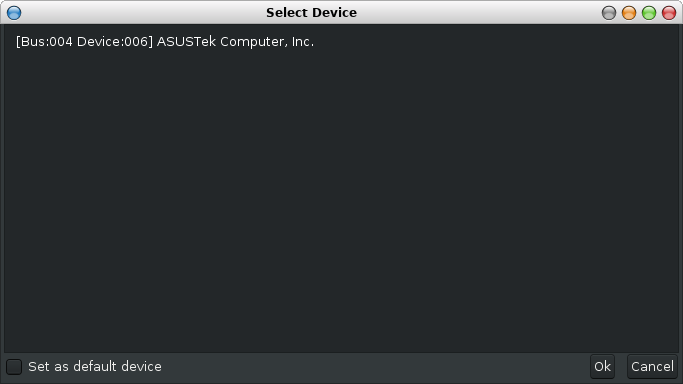
\includegraphics[width=\textwidth]{./Resources/device_selector}
	\caption{Seletor de dispositivos} 
	Fonte: Autor
	\label{fig:selecionar_dispositivo}
\end{figure}

\hfill
\par Ao selecionar o dispositivo, o usu�rio pode ativar a op��o "\textit{Set as default device}". Isso far� com que a op��o escolhida seja salva e n�o exibir� o seletor de dispositivos nas pr�ximas compila��es.
\par Se tudo ocorreu como o esperado, o usu�rio deve ver a mensagem de c�pia no \textit{console} abaixo do editor, conforme mostra a figura~\ref{fig:console_sucesso}.

\begin{figure}[h]
	\centering
	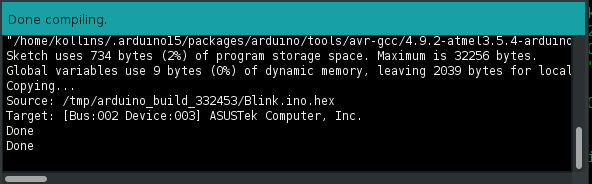
\includegraphics[width=\textwidth]{./Resources/copy_success}
	\caption{C�pia do arquivo realizada com sucesso para o \textit{smartphone}} 
	Fonte: Autor
	\label{fig:console_sucesso}
\end{figure}

\section{Simulador}
\label{resultado_sofia}

\par Ao abrir o simulador, o usu�rio � recebido com uma \textit{Splash Screen}, mostrada na figura~\ref{fig:splash_screen}, enquanto o banco de dados � carregado para a mem�ria principal, e posteriormente, o usu�rio � redirecionado para a tela inicial do simulador, mostrada na figura~\ref{fig:tela_inicial}

\begin{figure}[h]
	\centering
	
\includegraphics[width=0.25\textwidth]{./Resources/splash_screen}
	\caption{\textit{Splash Screen} exibida ao abrir o simulador} 
	Fonte: Autor
	\label{fig:splash_screen}
\end{figure}

\begin{figure}[H]
	\centering
	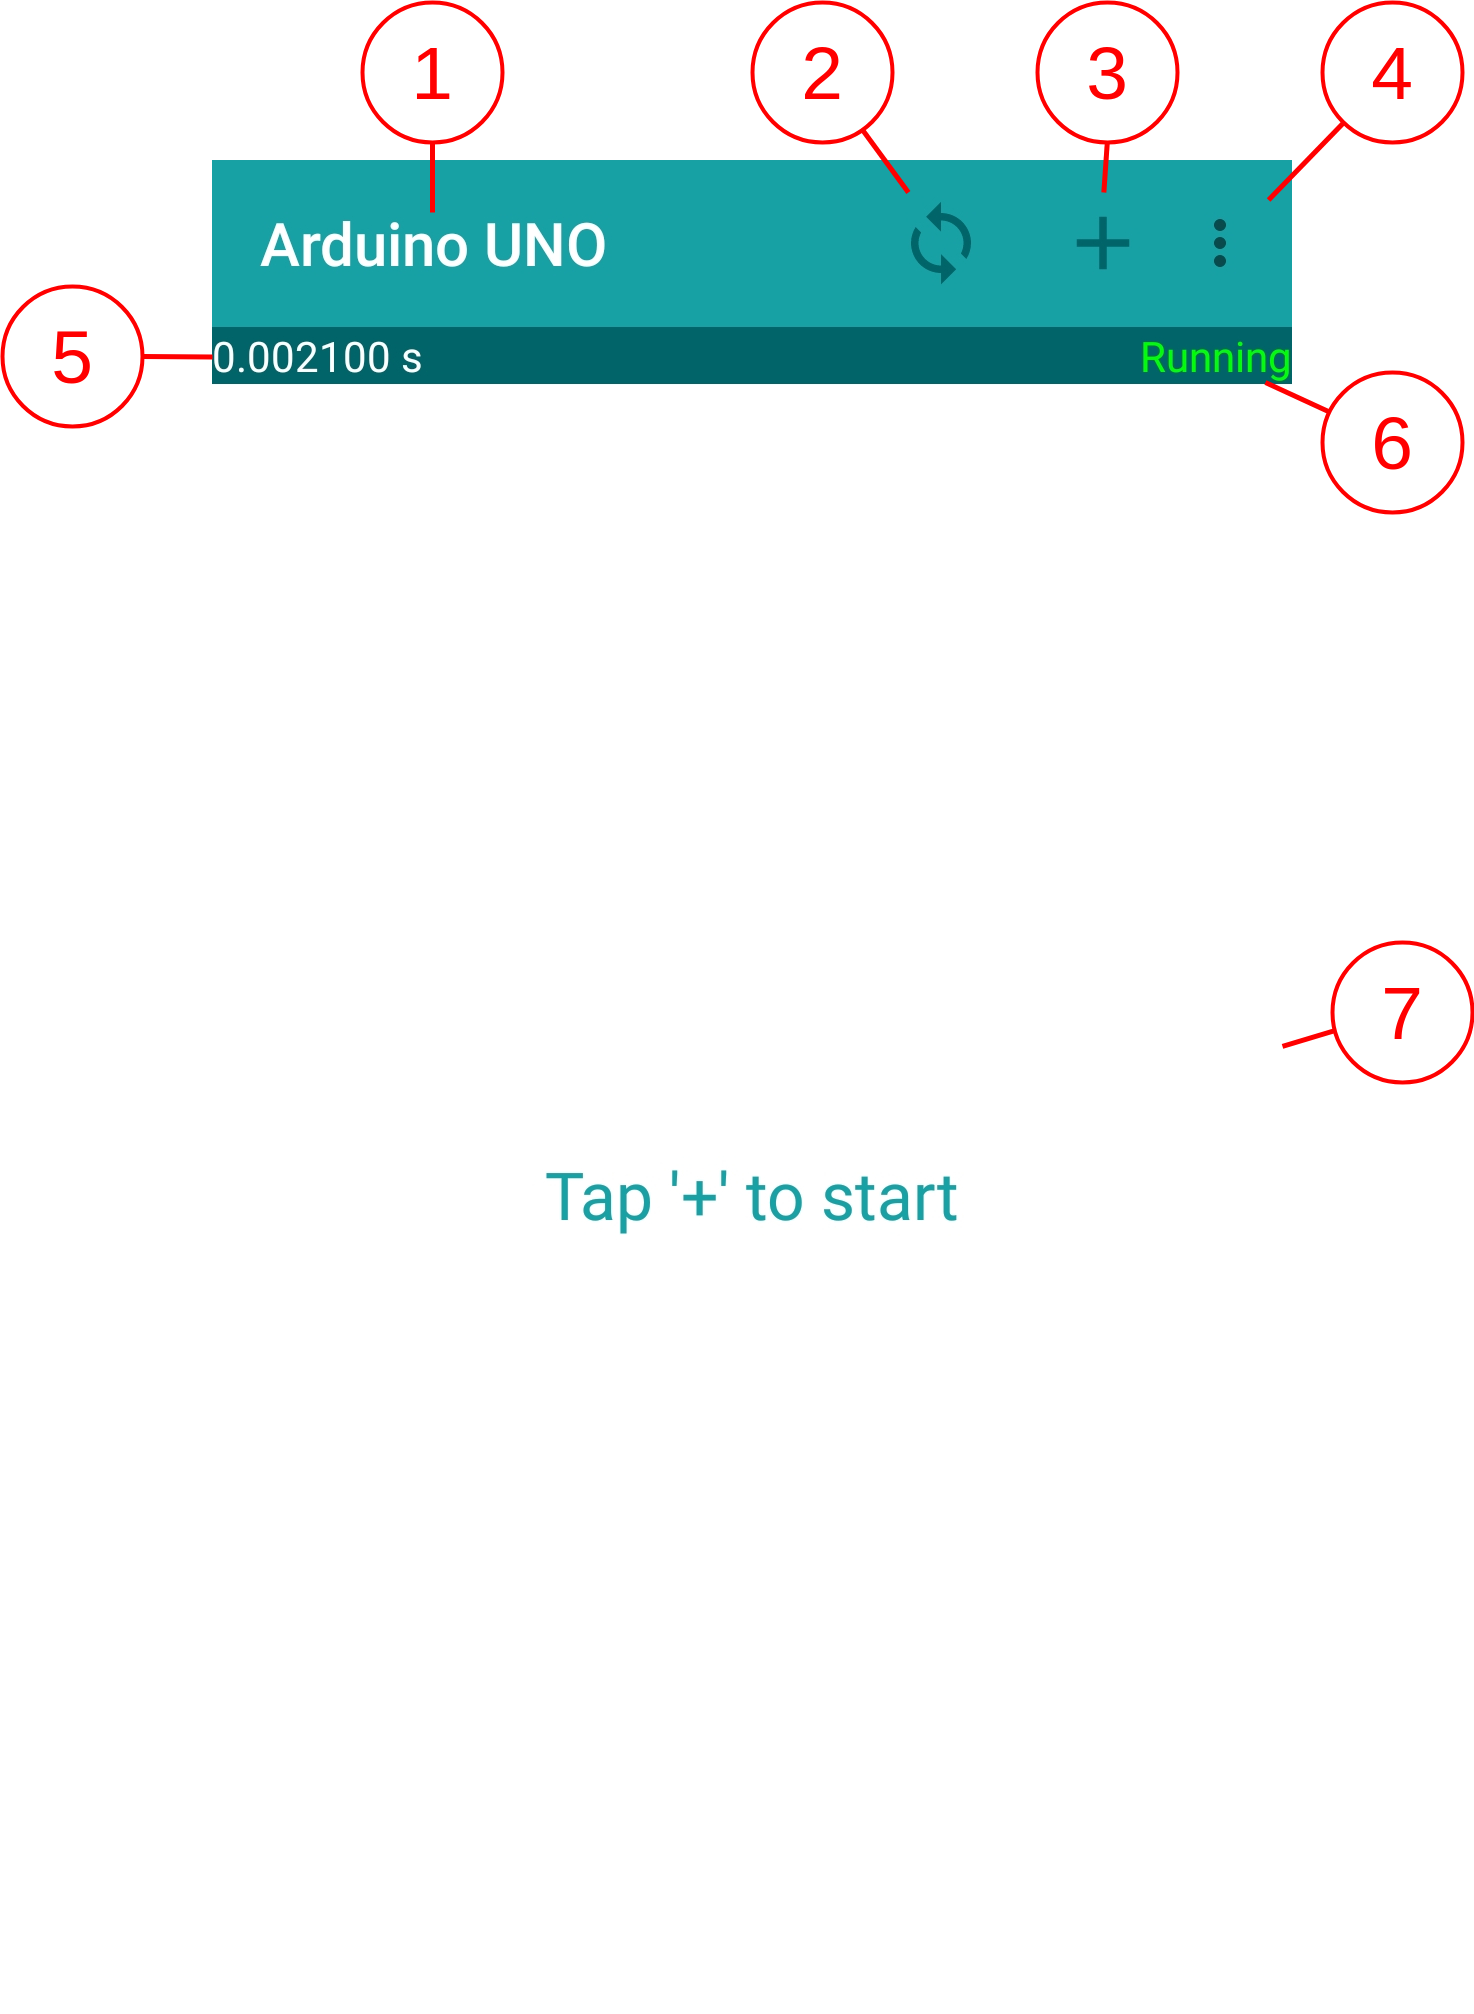
\includegraphics[width=0.45\textwidth]{./Resources/tela_inicial}
	\caption{Tela inicial do simulador} 
	Fonte: Autor
	\label{fig:tela_inicial}
\end{figure}

\par Na parte superior do simulador se concentram as op��es para que o usu�rio comece a utilizar o sistema, bem como informa��es sobre o estado da simula��o. Nesta \textit{toolbar}, o usu�rio tem acesso �s seguintes op��es/informa��es:

\begin{enumerate}
\item \textbf{Modelo simulado}: Mostra qual placa de Arduino est� sendo utilizada para a simula��o.
\item \textbf{Bot�o \textit{Reset}}: Permite o \textit{reset} manual do sistema.
\item \textbf{Adicionar Entrada/Sa�da}: Permite adicionar uma entrada/sa�da digital ou uma entrada anal�gica, bem como um monitor serial.
\item \textbf{Outras op��es}: Cont�m fun��es adicionais para importar c�digo do \textit{smartphone}, mapa de mem�ria, configura��o de tens�o de refer�ncia (para o conversor A/D), remover todas as entradas/sa�das, ajuda e acesso � informa��es do projeto.
\end{enumerate}

\par Al�m disso, o usu�rio pode visualizar:

\begin{enumerate}
	\setcounter{enumi}{4}
\item \textbf{Tempo simulado}: Exibe tempo simulado do sistema, baseado no cristal de 16MHz e atualizado a cada pulso de \textit{clock} interno do sistema.
\item \textbf{Status}: Mostra o \textit{status} da simula��o.
\item \textbf{�rea de Trabalho}: Onde ser�o dispostos os elementos de entrada e sa�da.
\end{enumerate}

\par Caso n�o seja encontrado um arquivo hexadecimal ou ocorra alguma falha em sua abertura, o usu�rio deve ver uma mensagem na barra de \textit{status} informando o problema, como mostrado na figura~\ref{fig:hex_file_not_found}.

\begin{figure}[h]
	\centering
	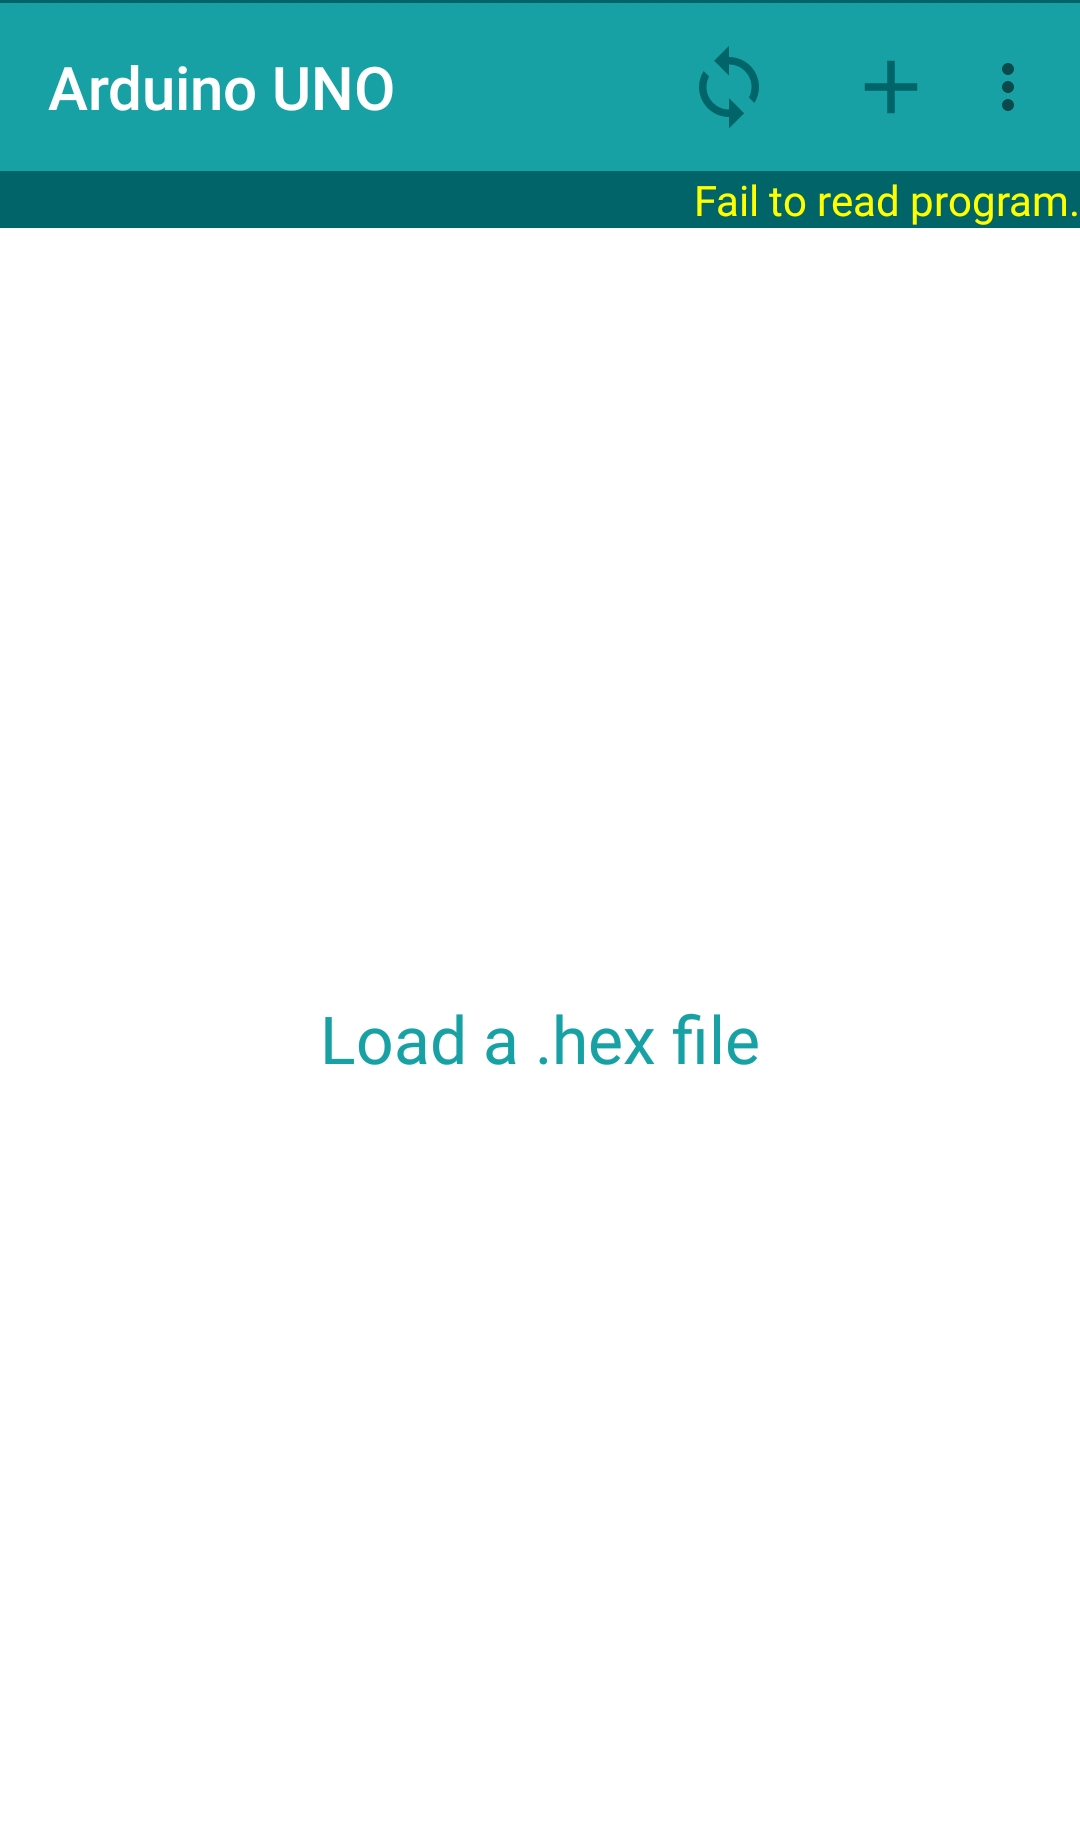
\includegraphics[width=0.35\textwidth]{./Resources/hex_file_not_found}
	\caption{Falha ao abrir arquivo hexadecimal} 
	Fonte: Autor
	\label{fig:hex_file_not_found}
\end{figure}

\subsection{Intera��o com o sistema}

\par O usu�rio interage com o sistema por meio de entradas e sa�das no simulador. Uma sa�da digital � mostrada na figura~\ref{fig:saida_digital}. No lado esquerdo � poss�vel selecionar o pino no qual a sa�da estar� conectada e do lado direito � mostrado o estado do pino. Por padr�o, o pino 13 � selecionado, uma vez que este � o pino onde o LED interno est� conectado no Arduino UNO. A figura~\ref{fig:saida_digital} mostra os tr�s estados poss�veis para uma sa�da no simulador.

\begin{figure}[H]
	\centering
	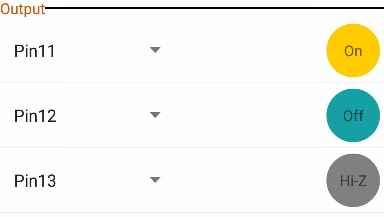
\includegraphics[width=0.55\textwidth]{./Resources/outputs}
	\caption{Sa�das digitais do simulador} 
	Fonte: Autor
	\label{fig:saida_digital}
\end{figure}

\vfill
\par Uma entrada pode ser digital ou anal�gica. Uma entrada digital � mostrada na figura~\ref{fig:entrada_digital}. Pode-se observar que existem 4 elementos em uma entrada digital, s�o eles (da esquerda para a direita):

\begin{figure}[h]
	\centering
	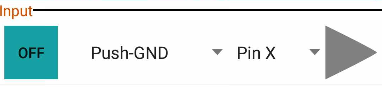
\includegraphics[width=0.60\textwidth]{./Resources/inputs}
	\caption{Entradas digitais do simulador} 
	Fonte: Autor
	\label{fig:entrada_digital}
\end{figure}

\begin{itemize}
\item \textbf{Bot�o}: por onde o usu�rio envia sinais ao o sistema.
\item \textbf{Seletor de modo}: define a opera��o do bot�o, podendo ser:
	\begin{itemize}
	\item Push-GND: envia n�vel baixo se pressionado, indefinido caso contr�rio (� a op��o padr�o).
	\item Push-VDD: envia n�vel alto se pressionado, indefinido caso contr�rio.
	\item Pull-Up: envia n�vel baixo se pressionado, alto caso contr�rio.
	\item Pull-Down: envia n�vel alto se pressionado, baixo caso contr�rio.
	\item Toggle: alterna seu n�vel a cada toque no bot�o.
	\end{itemize}
\item \textbf{Seletor de pino}: define para qual pino do Arduino o sinal deve ser enviado.
\item \textbf{Sa�da do sinal}: mostra o que est� sendo enviado para o pino selecionado
\end{itemize}

\par Por padr�o, nenhum pino est� selecionado. Isso garante que n�o haver� um curto-circuito ao adicionar uma entrada. Em caso de curto-circuito, � exibida uma mensagem na barra de status (como mostra a figura~\ref{fig:curto-circuito}) e a simula��o para, podendo ser reiniciada manualmente assim que a condi��o de curto-circuito for removida.

\begin{figure}[H]
	\centering
	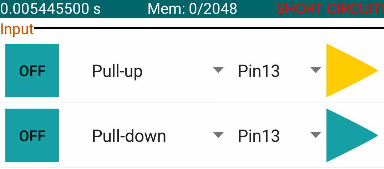
\includegraphics[width=0.45\textwidth]{./Resources/short_circuit}
	\caption{Condi��o de cuito-circuito entre entradas} 
	Fonte: Autor
	\label{fig:curto-circuito}
\end{figure}

\par Uma entrada anal�gica � mostrada na figura~\ref{fig:entrada_analogica}. Ela possui um seletor de pino, uma barra deslizante e um volt�metro, indicando o valor de tens�o enviado ao Arduino. Esta entrada permite ao usu�rio enviar valores de tens�o entre 0V e 5V e assim como na entrada digital, nenhuma entrada est� selecionada por padr�o.

\begin{figure}[h]
	\centering
	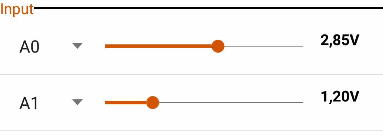
\includegraphics[width=0.45\textwidth]{./Resources/analog_input}
	\caption{Entradas anal�gicas do simulador} 
	Fonte: Autor
	\label{fig:entrada_analogica}
\end{figure}

\par Caso se queira remover uma entrada/sa�da, pode-se utilizar um toque longo na c�lula desejada e selecionar quais elementos ser�o removidos, como mostra a figura~\ref{fig:remocao}. Alternativamente, pode-se utilizar a op��o "\textit{Clear I/O}" da \textit{toolbar} para remover todas as entradas e sa�das.

\begin{figure}[H]
	\centering
	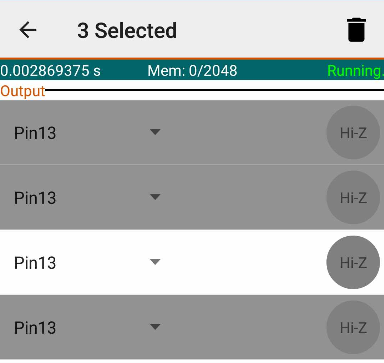
\includegraphics[width=0.35\textwidth]{./Resources/remocao}
	\caption{Remo��o manual de pinos de sa�da} 
	Fonte: Autor
	\label{fig:remocao}
\end{figure}

\subsection{Monitor Serial}

\par Outro modo de intera��o com o sistema � por meio do monitor serial, mostrado na figura~\ref{fig:monitor_serial}. Este monitor pode ser utilizado para receber ou enviar informa��es para a USART e ocupa o mesmo espa�o reservado para as sa�das digitais, ou seja, n�o � poss�vel visualizar as sa�das em conjunto com o monitor serial (� poss�vel, no entanto, utiliz�-lo simultaneamente com entradas). 

\begin{figure}[h!]
	\centering
	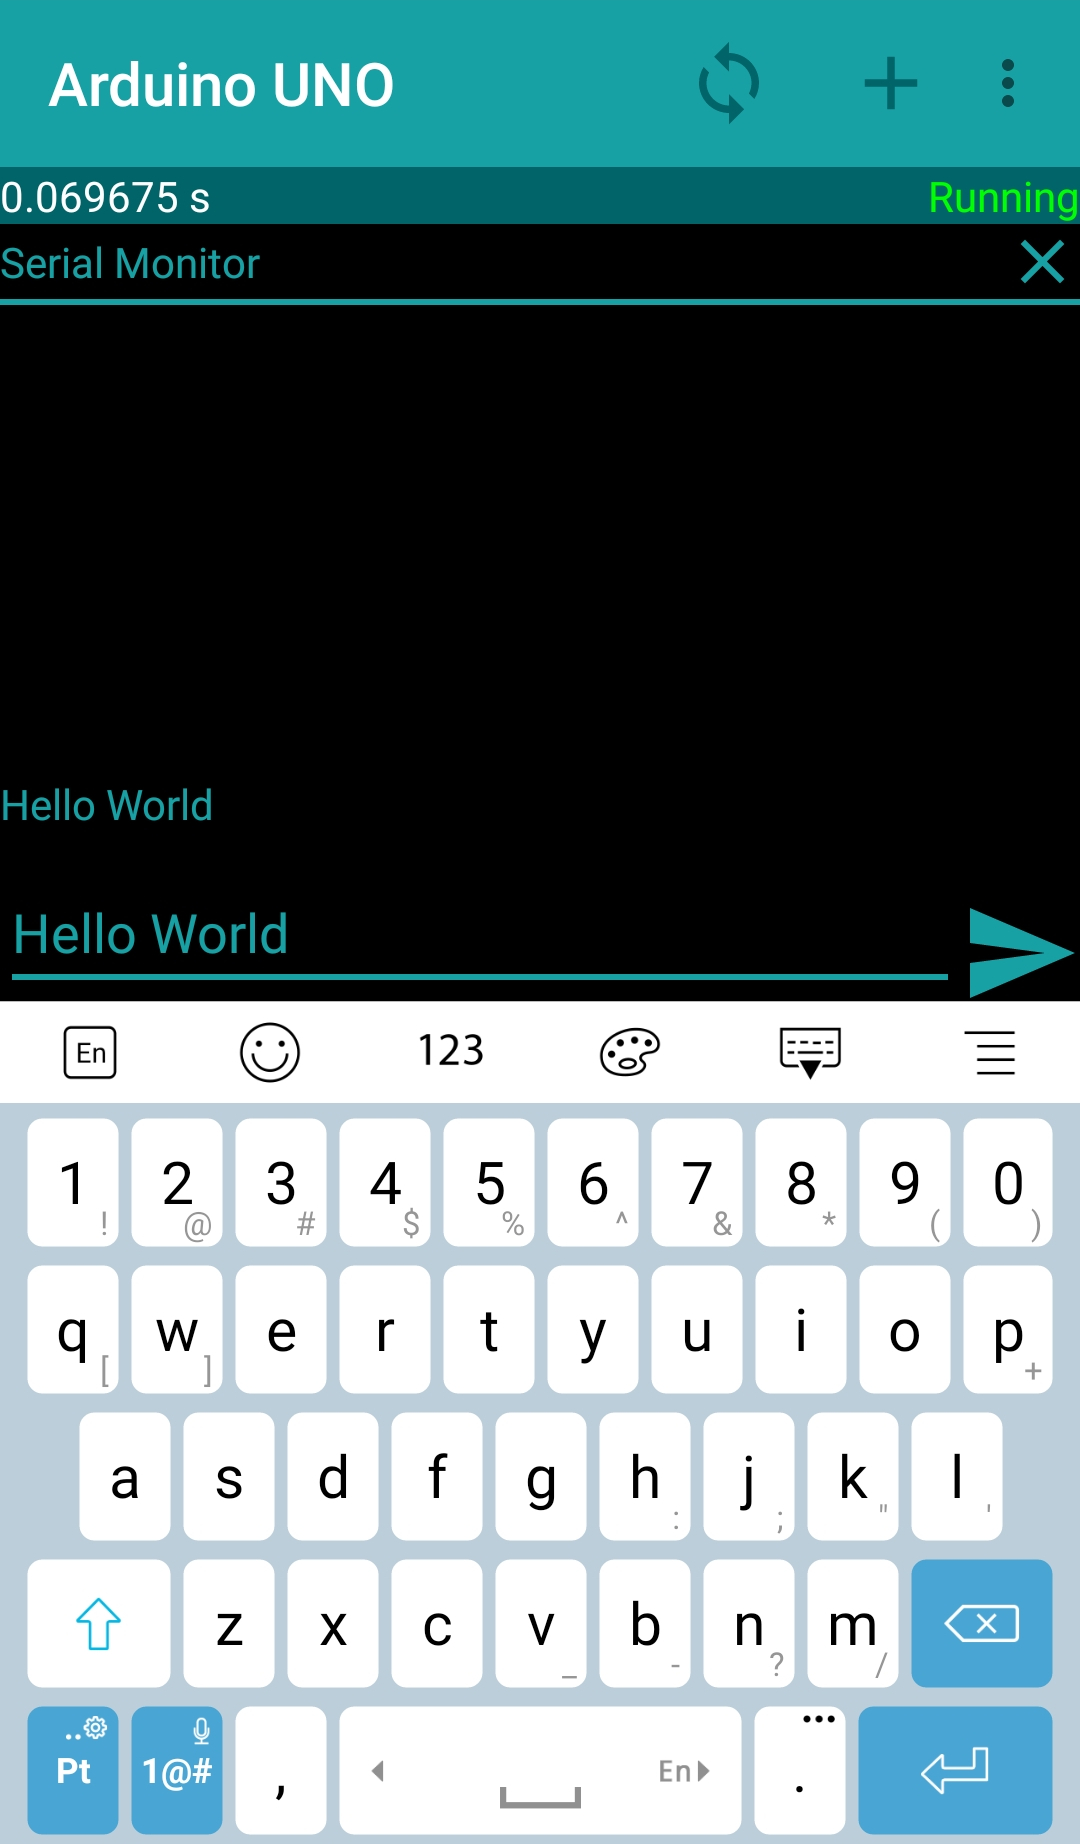
\includegraphics[width=0.25\textwidth]{./Resources/serial_monitor_working}
	\caption{Monitor Serial} 
	Fonte: Autor
	\label{fig:monitor_serial}
\end{figure}

\par O monitor serial pode ser removido tamb�m com a op��o "\textit{Clear I/O}" ou clicando no "x" na parte superior.

\subsection{Mapa de mem�ria}

\par O recurso de mapa de mem�ria � apresentado na figura~\ref{fig:mapa_memoria}. Este recurso permite ao usu�rio ver e acompanhar o estado de cada bit da mem�ria de dados enquanto a simula��o continua funcionando, bem como verificar qual o uso total de mem�ria pelo sistema em bytes e em porcentagem. O estado dos bits n�o � atualizado automaticamente na tela, mas sim a cada 800ms, diminuindo o impacto na performance do simulador quando este recurso � aberto.

\begin{figure}[h]
	\centering
	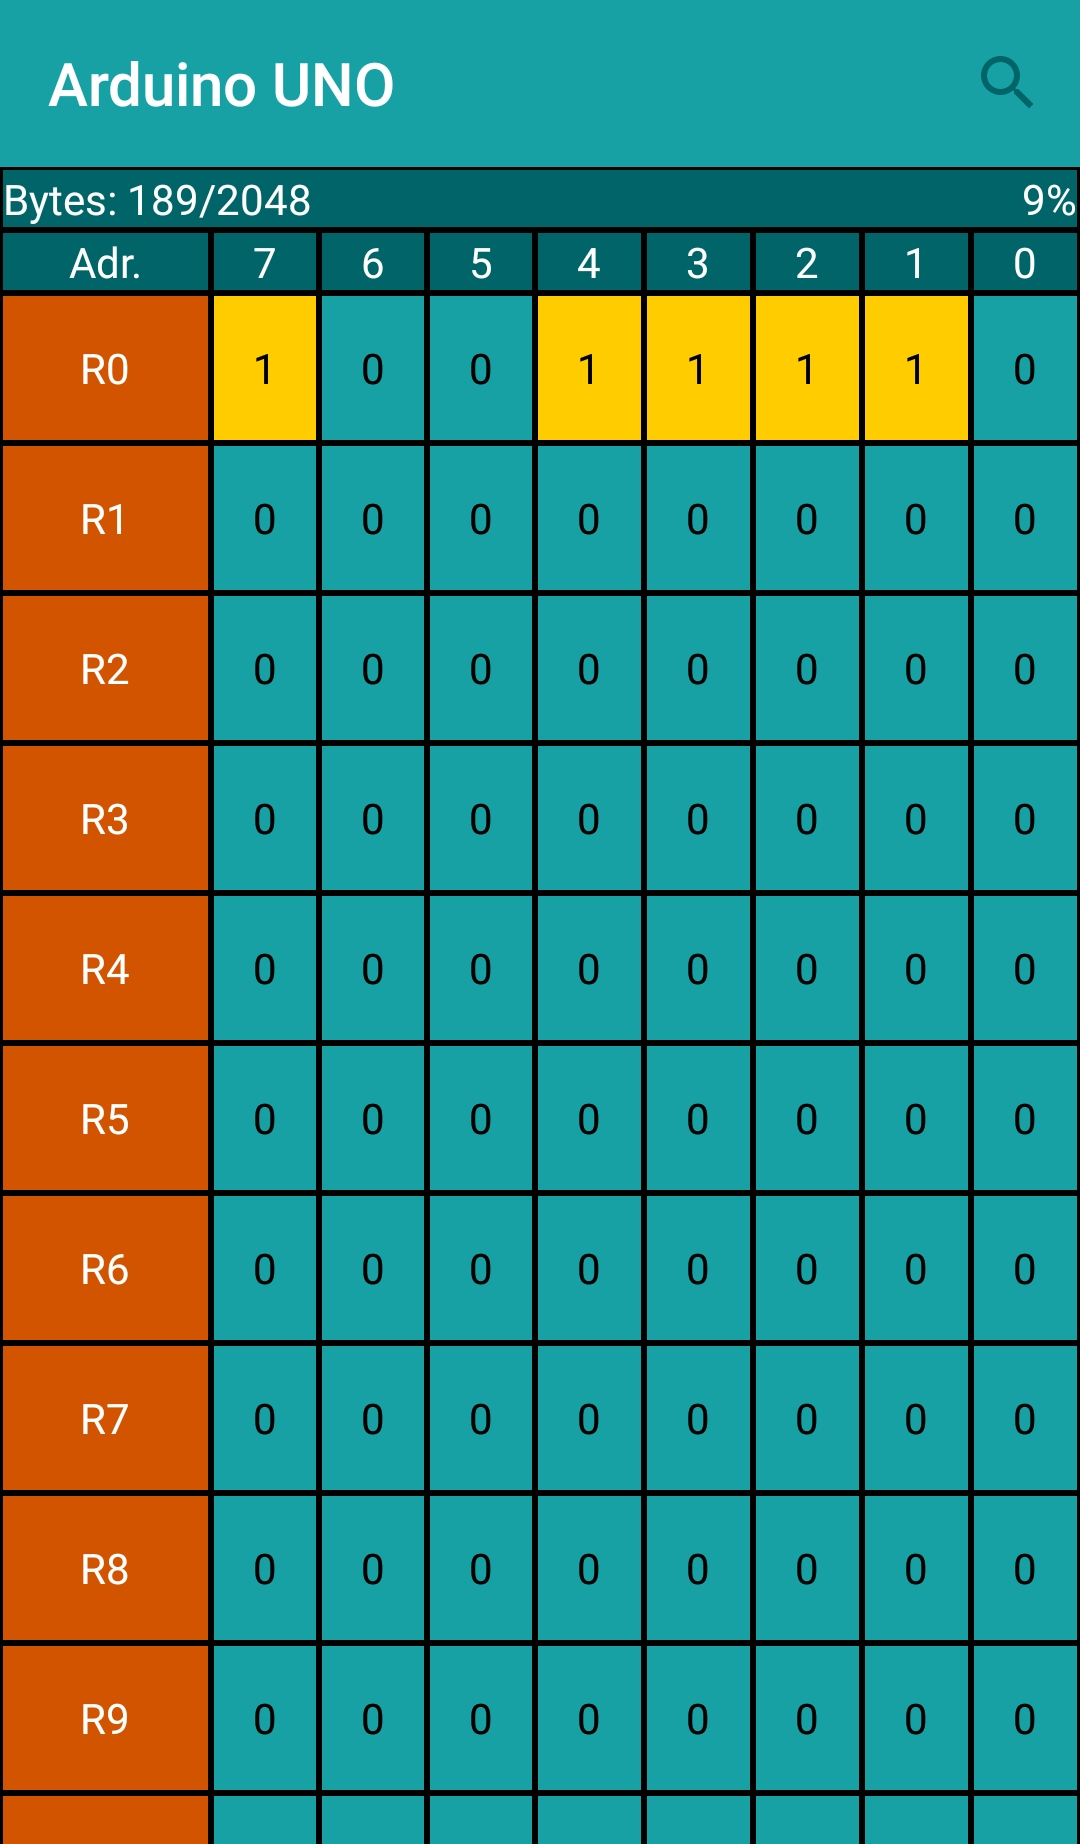
\includegraphics[width=0.20\textwidth]{./Resources/memory_map}
	\caption{Mapa de mem�ria} 
	Fonte: Autor
	\label{fig:mapa_memoria}
\end{figure}

\par Toda a mem�ria (2kB), somado aos registradores, podem ser visualizados com esta fun��o. Para facilitar a busca por um endere�o espec�fico, os registradores foram nomeados e adicionou-se o recurso de busca, que pode ser acessado pelo �cone de lupa no canto superior direito. A figura~\ref{fig:mapa_memoria_busca} mostra a busca sendo utilizada para encontrar o registrador TCNTx.

\begin{figure}[h]
	\centering
	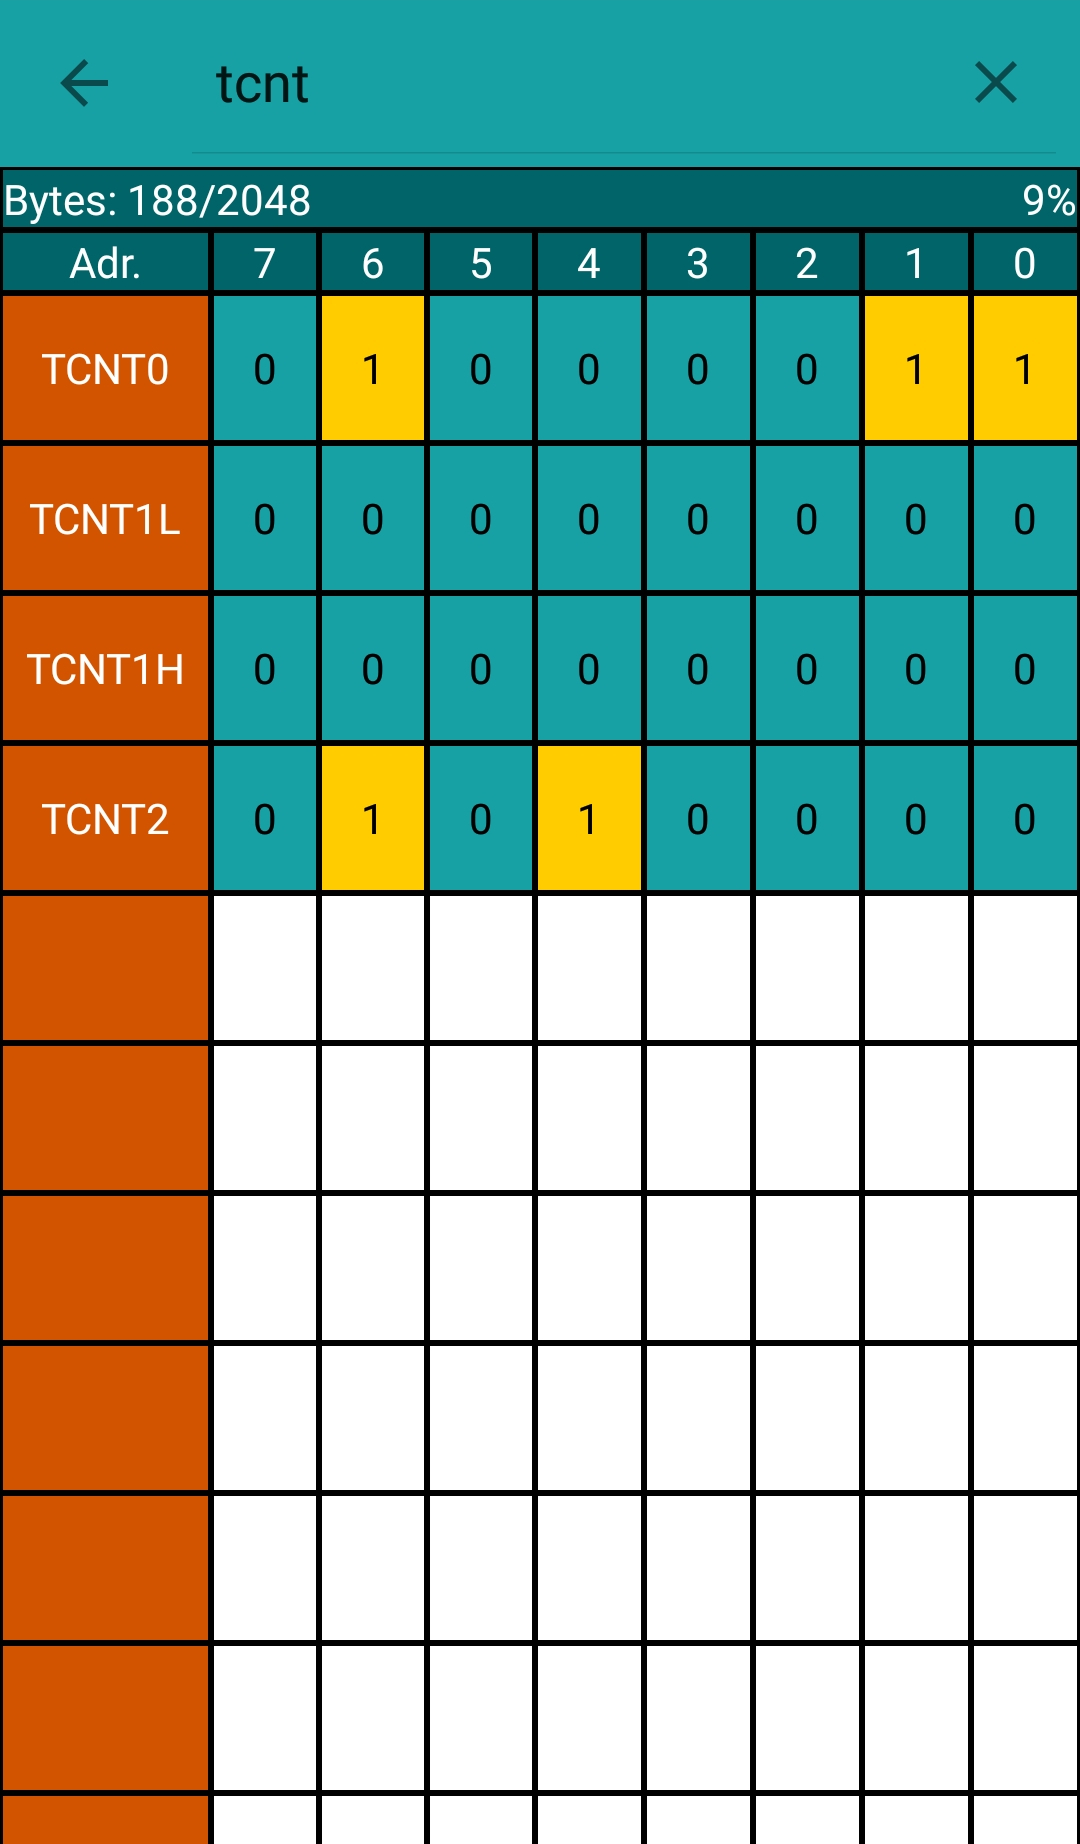
\includegraphics[width=0.20\textwidth]{./Resources/memory_map_search}
	\caption{Recurso de busca do mapa de mem�ria} 
	Fonte: Autor
	\label{fig:mapa_memoria_busca}
\end{figure}

\subsection{Refer�ncia externa de tens�o}

\par Outro recurso que foi inserido no simulador foi a configura��o da refer�ncia externa de tens�o para convers�o anal�gica. Em \textit{hardware}, esta refer�ncia � aplicada no pino AREF e utilizada como base para convers�o. No simulador, pode-se utilizar o menu "\textit{AREF Config}" para simular esta fun��o. A figura~\ref{fig:aref_config} mostra a tela de configura��o exibida.

\begin{figure}[h]
	\centering
	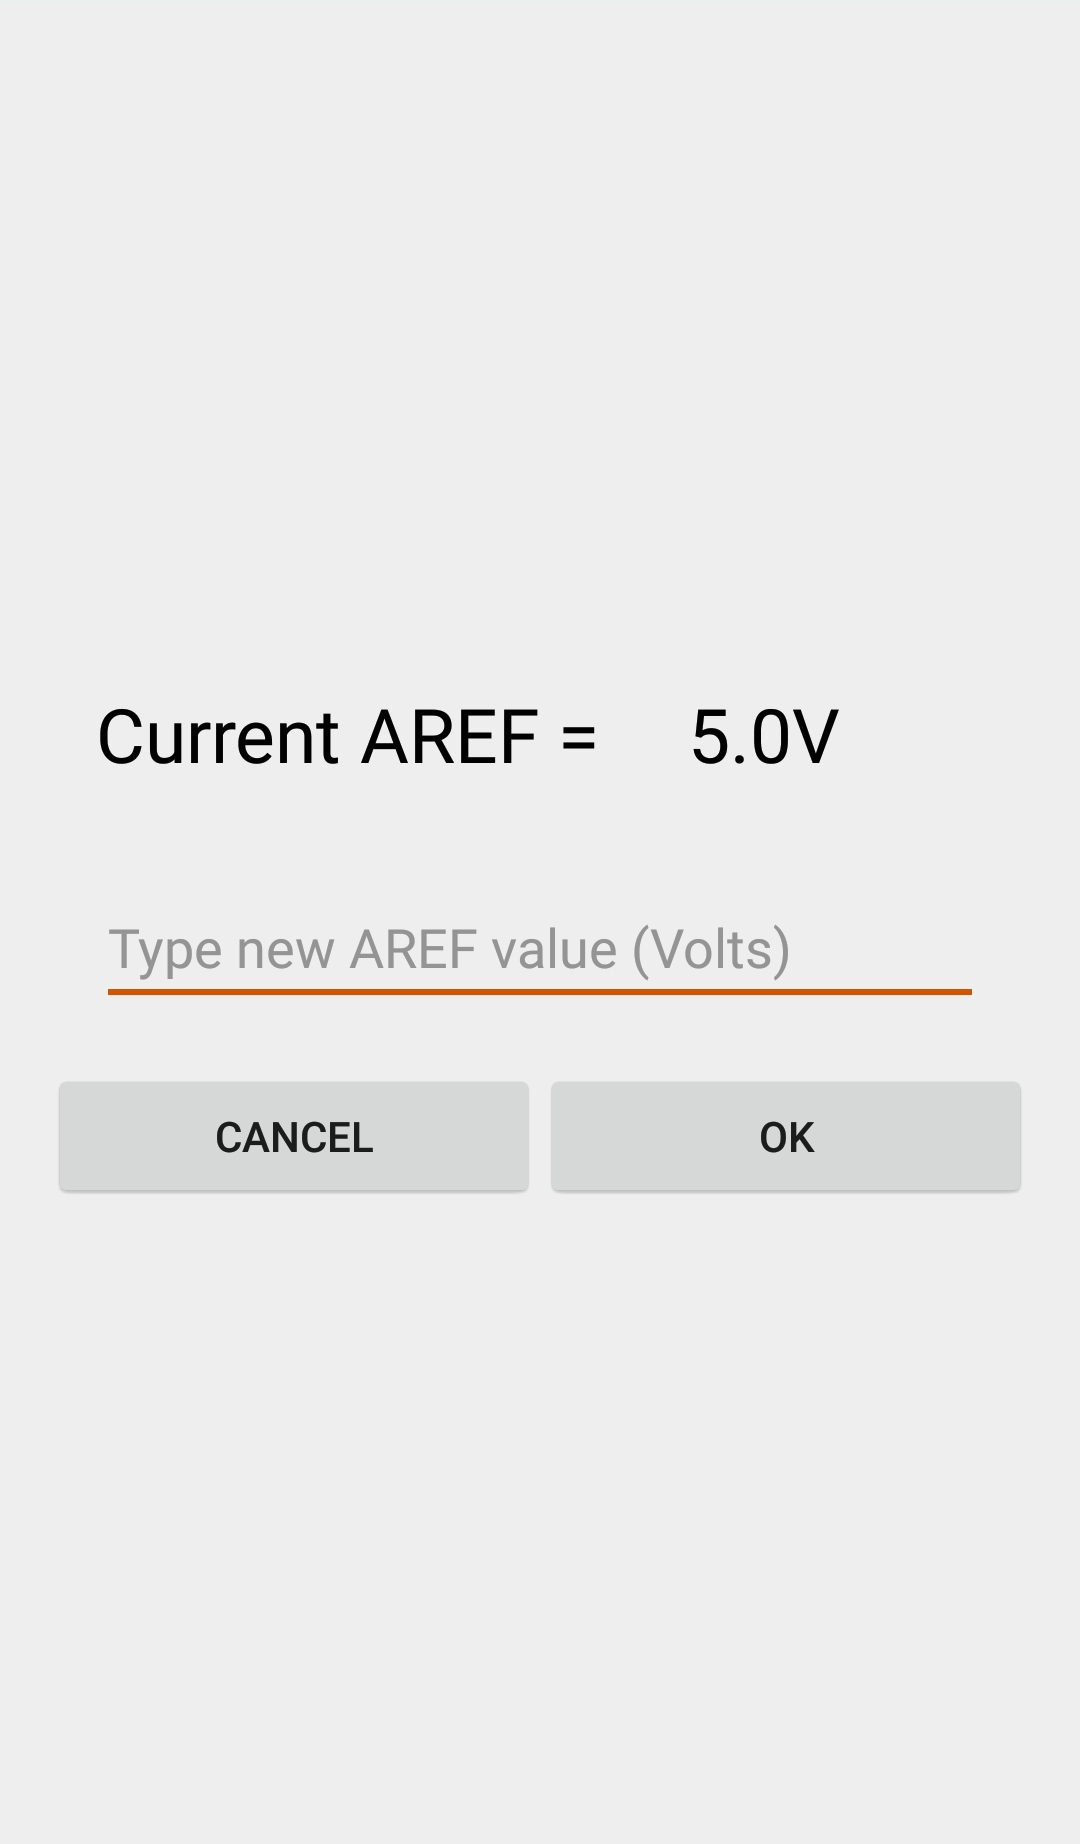
\includegraphics[width=0.25\textwidth]{./Resources/AREF_config}
	\caption{Configura��o de tens�o externa aplicada ao pino AREF, usada como base para convers�o A/D} 
	Fonte: Autor
	\label{fig:aref_config}
\end{figure}

\par Por padr�o, o valor configurado � de 5V (como mostra a figura~\ref{fig:aref_config}). Este valor pode ser alterado para qualquer valor real que esteja dentro das epecifica��es m�nimas e m�ximas apresentadas na folha de dados do ATmega328P (M�nimo: 1V, M�ximo: 5V).

\subsection{Medi��o de frequ�ncia}

\par Caso a frequ�ncia de oscila��o de um pino de sa�da seja muito alta, o simulador n�o ser� capaz de exibir esta intermit�ncia corretamente devido a limita��es de velocidade da atualiza��o da tela do Android (m�ximo 60fps). Nestes casos, pode-se utilizar o recurso de frequenc�metro integrado ao simulador para verificar a qual frequ�ncia a sa�da est� alterando seu estado. (Na verdade, pode-se utilizar o frequenc�metro em qualquer ocasi�o, este � apenas um caso onde seu uso se faz absolutamente necess�rio para depura��o.)

\par Para medir frequ�ncia em um pino de sa�da, basta pressionar a sa�da desejada com um toque longo e selecionar frequenc�metro (figura~\ref{fig:frequencimetro_icone}). Os valores de frequ�ncia e \textit{duty cicle} aparecer�o na c�lula de sa�da, como mostra a figura~\ref{fig:frequencimetro}.

\begin{figure}[h]
	\centering
	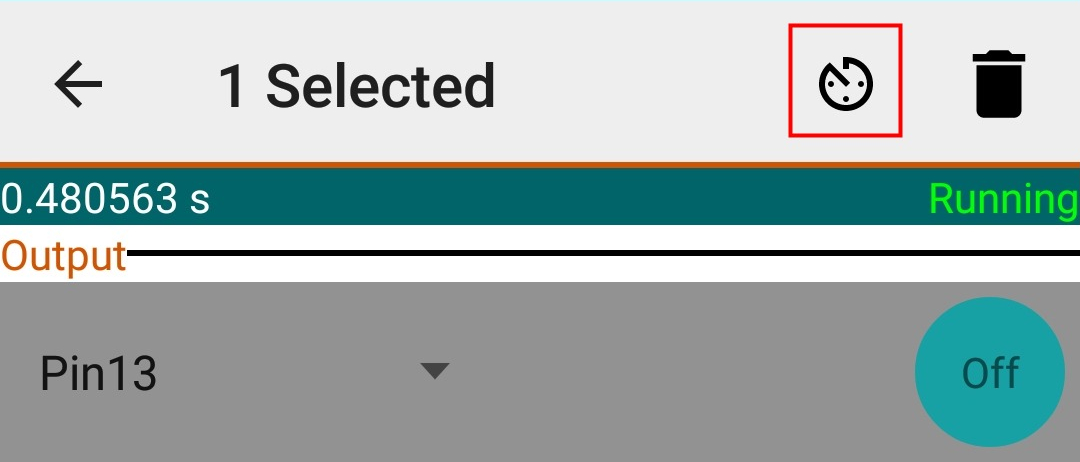
\includegraphics[width=0.5\textwidth]{./Resources/frequency_meter_icon}
	\caption{�cone do frequenc�metro} 
	Fonte: Autor
	\label{fig:frequencimetro_icone}
\end{figure}

\begin{figure}[H]
	\centering
	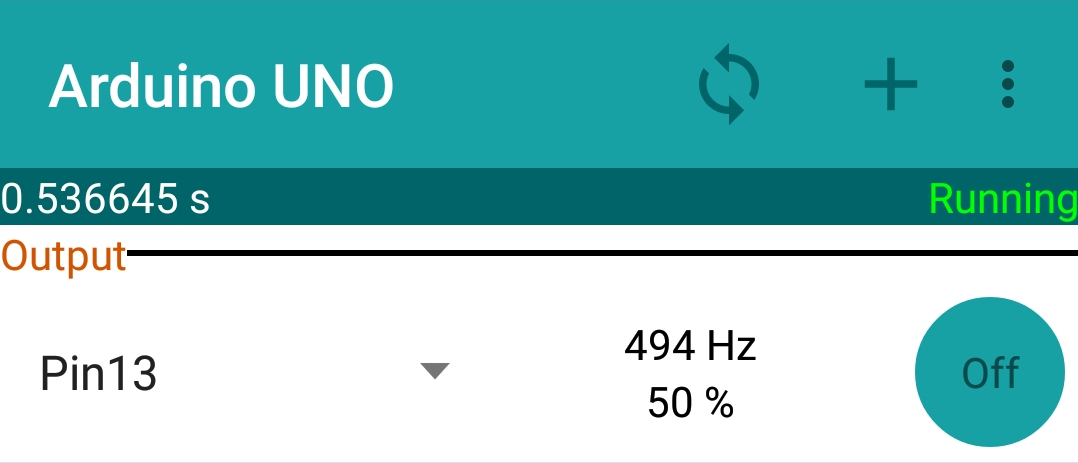
\includegraphics[width=0.5\textwidth]{./Resources/frequency_meter}
	\caption{Frequenc�metro em funcionamento} 
	Fonte: Autor
	\label{fig:frequencimetro}
\end{figure}

\par A medi��o de frequ�ncia implementada se mostrou bastante precisa quando comparada com as medi��es reais de frequ�ncia. Para realizar os testes, foram utilizados os projetos \textit{Blink} e \textit{Timer1}, apresentados nos ap�ndices~\ref{apendice_blink} e~\ref{apendice_timer} respectivamente. O projeto \textit{Blink} foi utilizado ora com a fun��o \textit{delay}, ora com fun��o \textit{delayMicroseconds}, desta forma podendo obter diferentes valores de frequ�ncia gerados por diferentes m�todos, enquanto o projeto \textit{Timer1} foi configurado com diferentes valores em TCNT1 para as diferentes configura��es de frequ�ncia e \textit{duty cycle}. As tabelas~\ref{tab:comparacao_frequencia} e~\ref{tab:comparacao_duty} apresentam os valores medidos de frequ�ncia obtidos com o simulador e com o oscilosc�pio ligado ao Arduino, bem como o erro relativo de cada medi��o comparado com o valor te�rico esperado. 

\par Como pode ser observado, o simulador e o Arduino se comportam de maneira semelhantes tanto na medi��o de frequ�ncia quanto nas relativas ao \textit{duty cicle}, apresentando um erro relativo alto quando se trabalha com altas frequ�ncias. 

\par Com isso, conclui-se que o frequenc�metro incluso no simulador fornece medi��es satisfat�rias, principalmente se a aplica��o desenvolvida n�o tiver grandes exig�ncias quanto � estes par�metros. Notou-se apenas uma certa instabilidade nos valores quando as medi��es eram feitas em altas frequ�ncias, mas nada cr�tico ao ponto de n�o permitir o uso e a leitura das grandezas.

\begin{table}[p]
	\centering
	\caption{Compara��o das medi��es de frequ�ncia (\textit{duty cycle: 50\%}). Foram coletadas 110 amostras em cada frequ�ncia medida}
	\label{tab:comparacao_frequencia}
	\begin{tabular}{|c|c|c|c|c|c|c|c|}
		\hline
		\multirow{3}{*}{\textbf{Fun��o}} & \multirow{3}{*}{\textbf{Per�odo}} & \multicolumn{4}{c|}{\textbf{Frequ�ncia (Hz)}}                                             & \multicolumn{2}{c|}{\textbf{Erro (\%)}}                 \\ \cline{3-8} 
		&  & \multicolumn{2}{c|}{SOFIA} & \multicolumn{2}{c|}{Arduino} & \multirow{2}{*}{SOFIA} & \multirow{2}{*}{Arduino} \\ \cline{3-6}
		&\textbf{(Te�rico)}  & M�dia & D. Padr�o & M�dia & D. Padr�o           &                   &                   \\ \hline
		\multirow{3}{*}{\textit{\small{delayMicroseconds}}} 
		& 2 $\mu$s & 107.062 & 37.946 & 133.254 & 4,93          
		& 78,59 & 73,35 \\ \cline{2-8} 
		& 0,5 ms & 1.967 & 12,04 & 1.968 & 11,97           
		& 1,63 & 1,58  \\ \cline{2-8} 
		& 1 ms & 989,16 & 0,98 & 988,36 & 0,03    
		& 1,08 & 1,16                   \\ \hline
		\multirow{3}{*}{\textit{\small{delay}}}
		& 2 ms & 495,71 & 0,55 & 495,44 & 9,47
		& 0,86 & 0,91 \\ \cline{2-8} 
		& 4 ms & 248,96 & 0,19 & 248,64 & 0,21 
		& 0,41 & 0,55 \\ \cline{2-8} 
		& 8 ms & 125 & 0 & 124,59 & 0,03 
		& 0 & 0,32 \\ \hline
		\multirow{4}{*}{\textit{\small{Timer 1}}}
		& 125 ns & 33.991 & 3.187 & 39.778 & 1,01          
		& 99,58  & 99,5                  \\ \cline{2-8} 
		& 2,048 ms & 484 & 0 & 483,52 & 0,16   
		& 0,88 & 0,97 \\ \cline{2-8} 
		& 4,129 ms & 242,99 & 0,09 & 242,88 & 0,06
		& 0,33 & 0,28  \\ \cline{2-8} 
		& 8,192 ms & 122 & 0 & 121,72 & 0,01
		& 0,06 & 0,28                  \\ \hline
	\end{tabular}
\end{table}

\begin{table}[p]
	\centering
	\caption{Compara��o das medi��es de \textit{duty cicle} (projeto: \textit{Timer1}, frequ�ncia: 488Hz). Foram coletadas 111 amostras para cada valor de \textit{duty cycle} medido}
	\label{tab:comparacao_duty}
	\begin{tabular}{|c|c|c|c|c|c|c|}
		\hline
		\multicolumn{5}{|c|}{\textbf{Duty Cycle (\%)}}        & \multicolumn{2}{c|}{\textbf{Erro (\%)}}                 \\ \hline
		\multirow{2}{*}{Te�rico} & \multicolumn{2}{c|}{SOFIA} & \multicolumn{2}{c|}{Arduino} & \multirow{2}{*}{SOFIA} & \multirow{2}{*}{Arduino} \\ \cline{2-5}
		& M�dia & D. Padr�o & M�dia & D. Padr�o &                   &                   \\ \hline
		1  & 2  & 0 & 2,11  & 0,002 & 100 & 111             \\ \hline
		25 & 26 & 0 & 25,58 & 0,034 & 4   & 2,31            \\ \hline
		50 & 50 & 0 & 50,01 & 0,012 & 0   & 0,01            \\ \hline
		75 & 74 & 0 & 74,43 & 0,003 & 1,33& 0,76             \\ \hline
		99 & 98 & 0 & 97,90 & 0,002 & 1,01& 1,11             \\ \hline
	\end{tabular}
\end{table}

\section{M�tricas de \textit{Software}}

\subsection{An�lise Est�tica}

\par Com o uso do SonarQube, foi realizada a analise est�tica do c�digo com o objetivo principal de identificar e corrigir problemas relacionados � seguran�a, vulnerabilidades e manutenibilidade. O SonarQube fornece diversas m�tricas a respeito do projeto, al�m de classificar a qualidade do \textit{software} com notas variando de A (melhor qualidade) a E (pior qualidade).
\par A primeira m�trica relevante que a ferramenta fornece � uma medida de confiabilidade do sistema, baseada no n�mero de \textit{bugs}. A figura~\ref{fig:confiabilidade} mostra um gr�fico relacionando cada classe do projeto com a quantidade de \textit{bugs} encontrados (tempo para corre��o dos defeitos). Pode-se observar que uma classe se destaca pela sua quantidade de \textit{bugs}, esta classe � a \textit{DataMemory\_ATmega328P}.

\begin{figure}[h]
	\centering
	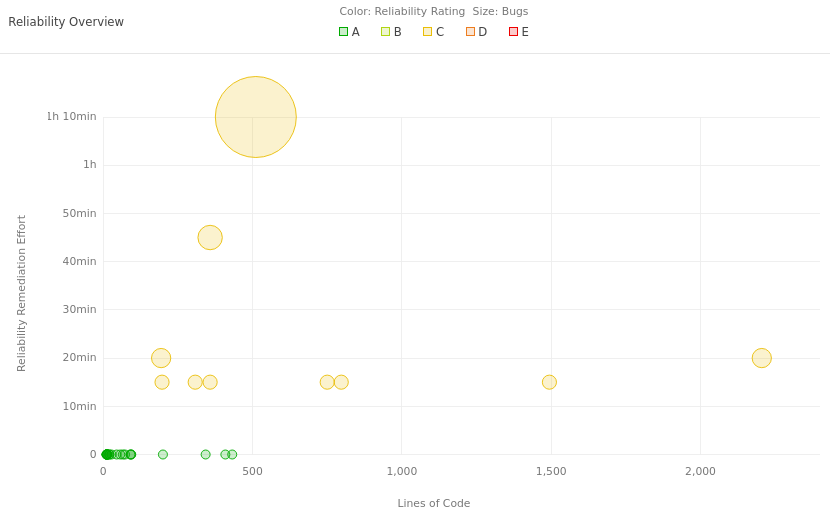
\includegraphics[width=\textwidth]{./Resources/confiabilidade}
	\caption{Gr�fico linhas de c�digo x esfor�o para resolu��o dos \textit{bugs}} 
	Fonte: Autor
	\label{fig:confiabilidade}
\end{figure}
 
\par � importante ressaltar que, por ser uma ferramenta de an�lise est�tica, muitos problemas apontados podem n�o se aplicar ao projeto ou ser falsos positivos. Em se tratando de \textit{bugs}, dos problemas que n�o foram resolvidos sobraram apenas \textit{bugs} relacionados ao tratamento de exce��es (que est� sendo feito com o uso de \textit{Logs}, no Android Studio) e � convers�o (\textit{cast}) de valores (os casos de teste criados com o JUnit4 est�o testando estas convers�es). Devido � estes problemas o sistema receberia classifica��o C em termos de confiabilidade, no entanto foi atribu�da a nota E devido � um \textit{bug} identificado na classe \textit{DataBaseHelper} relacionado � abertura e fechamento do banco de dados (apesar deste ter sido corrigido conforme a sugest�o proposta).

\par Outra m�trica fornecida diz respeito � seguran�a do sistema e se baseia na quantidade de vulnerabilidades encontradas. A figura~\ref{fig:seguranca} apresenta um gr�fico relacionando cada classe do projeto com a quantidade de vulnerabilidades (tempo para corre��o dos defeitos). Novamente, observa-se uma classe em destaque, esta � a \textit{OutputFragment\_Atmega328P}.

\begin{figure}[h]
	\centering
	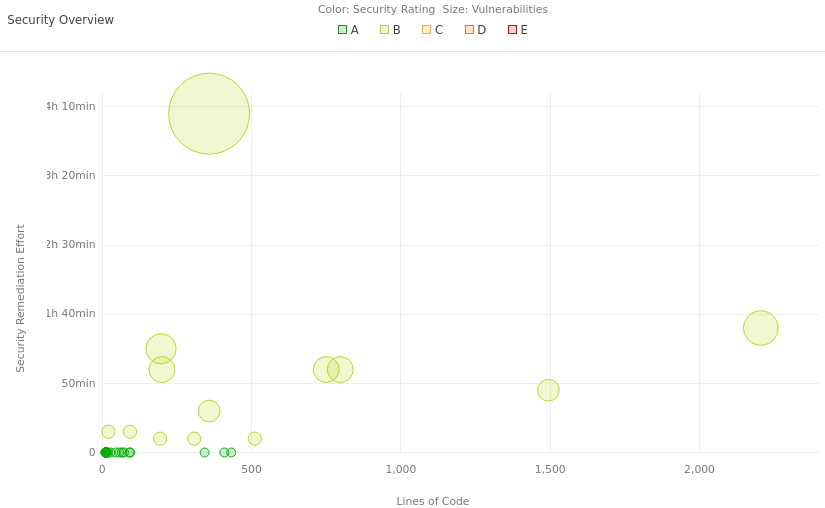
\includegraphics[width=\textwidth]{./Resources/seguranca}
	\caption{Gr�fico linhas de c�digo x esfor�o para resolu��o das vulnerabilidades} 
	Fonte: Autor
	\label{fig:seguranca}
\end{figure} 

\par Em termos de vulnerabilidades, o sistema apresenta melhores resultados em compara��o aos \textit{bugs}. Das que n�o foram resolvidas, sobraram apenas vulnerabilidades relacionadas � manipula��o de vari�veis est�ticas. Muitas destas, no entanto, s�o vari�veis privadas, de forma que n�o existem grandes problemas relacionado com o acesso delas por classes externas (como foi apontado pela ferramenta). O sistema foi classificado com o \textit{ranking} B para seguran�a.

\par A pr�xima m�trica obtida diz respeito a manutenibilidade do c�digo. Esta medida � feita com base na compexidade cognitiva dos m�todos e quanto ao uso devido/indevido de padr�es de codifica��o (esses s�o chamados \textit{Code Smells}). A figura~\ref{fig:manutencao} apresenta um gr�fico relacionando cada classe do projeto com a quantidade de \textit{Code Smells} encontrados (tempo para corre��o dos defeitos). A classe com maior n�mero de problemas para essa m�trica � a \textit{Timer1\_ATmega328P}.

\begin{figure}[H]
	\centering
	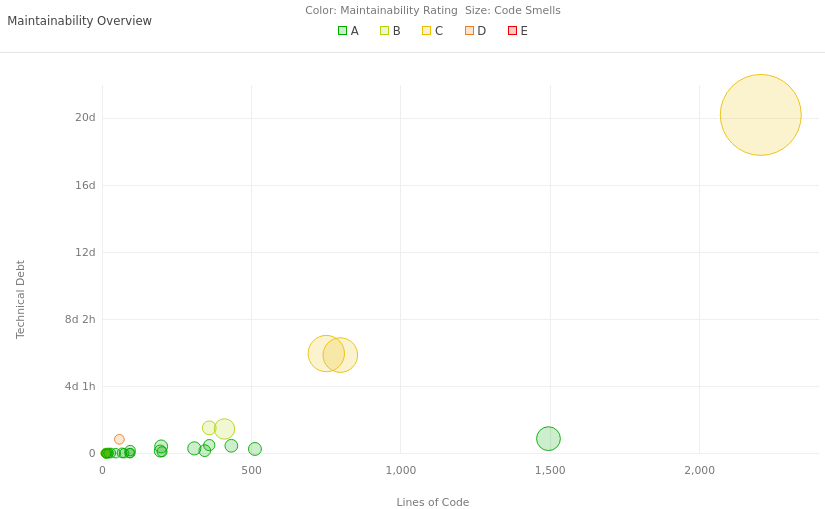
\includegraphics[width=\textwidth]{./Resources/manutencao}
	\caption{Gr�fico linhas de c�digo x esfor�o para resolu��o dos \textit{Code Smells}} 
	Fonte: Autor
	\label{fig:manutencao}
\end{figure} 

\par Muitos dos problemas apontados nesta categoria s�o de menor import�ncia, tais como remover linhas comentadas, mudar nomes de vari�veis, etc. Os problemas de maior import�ncia s�o os de complexidade cognitiva, que indicam que um m�todo est� muito grande, tornando-o de dif�cil compreens�o. No entanto, alguns destes m�todos n�o podem ser refatorados facilmente, j� que comprometeria a arquitetura geral do projeto.
\par Outro problema apontado quanto � manutenibilidade foi a quantidade de n�veis de heran�a que algumas classes possuem, excedendo o limite de 5 n�veis. N�o h� muito o que fazer nestes casos, j� que estas classes n�o herdam de nenhum c�digo desenvolvido, mas de classes do pr�prio sistema Android (como � o caso da classe \textit{AppCompatActivity}). Este foi o principal motivo para que o sistema fosse classificado com o \textit{ranking} C para manutenibilidade.

\par Tamb�m foi obtida uma m�trica de c�digo duplicado. A figura~\ref{fig:duplicacao} apresenta um gr�fico relacionando cada classe do projeto com a quantidade de linhas de c�digo duplicadas. 

\begin{figure}[h]
	\centering
	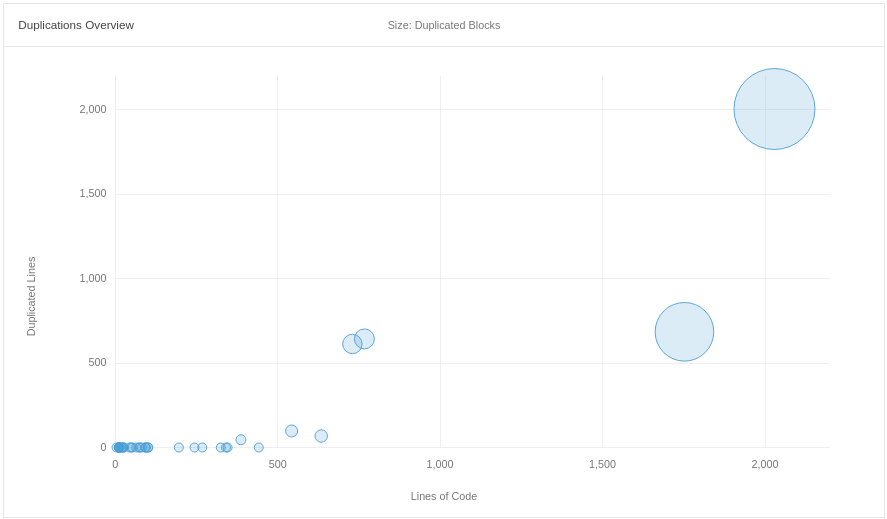
\includegraphics[width=\textwidth]{./Resources/duplicacao}
	\caption{Gr�fico linhas de c�digo x linhas de c�digo duplicadas.} 
	Fonte: Autor
	\label{fig:duplicacao}
\end{figure} 

\par As classes com maior n�mero de c�digo duplicado s�o as classes referentes aos temporizadores (o \textit{Timer1} � a classe em destaque na figura~\ref{fig:duplicacao}) e a CPU. Os modos de opera��o dos \textit{Timers} se assemelham em muitos aspectos, no entanto, escrever um �nico m�todo para gerenciar todos estes modos certamente o tornaria grande e complexo (gerando um problema na m�trica de complexidade cognitiva) e portanto, foram criados diferentes m�todos, cada um com pequenas varia��es, de forma a atender o modo de opera��o configurado. Um problema semelhante ocorre com a CPU, j� que v�rias instru��es realizam a leitura e a escrita dos valores na mem�ria de maneira id�ntica, mas suas opera��es s�o diferentes de modo que tamb�m n�o � poss�vel unir c�digos de diferentes instru��es.

\par A �ltima m�trica importante de ser mencionada � a de complexidade ciclom�tica. Esta � uma media interessante pois diz qual � o n�mero m�nimo de casos de teste necess�rios para que eles cubram todo o projeto. O valor obtido para complexidade ciclom�tica foi de 1.969.

\subsection{Cobertura}

\par Foram criados teste de unidade para todos os principais m�dulos do projeto (CPU, mem�rias de dado e de programa, conversor A/D, temporizadores, USART e m�dulo de interrup��o), totalizando 808 casos de teste. O foco dos testes foi a cobertura de linhas e condicionais e an�lise de valor limite, este �ltimo aplicado principalmente aos testes da CPU.

\par A cobertura dos testes criado foi medida tanto com a ferramenta interna do Android Studio quanto com o plugin JaCoCo (integrado ao SonarQube). Houve uma diferen�a de 10\% nas duas medidas de cobertura por estas ferramentas, com o Android Studio registrando 59\% de cobertura e o JaCoCo 49\%, como mostram as figuras~\ref{fig:cobertura_android_studio} e~\ref{fig:cobertura_jacoco}

\begin{figure}[H]
	\centering
	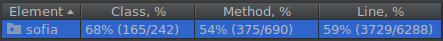
\includegraphics[width=0.65\textwidth]{./Resources/cobertura_android_studio}
	\caption{Medida de cobertura do projeto obtida com o  Android Studio} 
	Fonte: Autor
	\label{fig:cobertura_android_studio}
\end{figure}

\begin{figure}[h!]
	\centering
	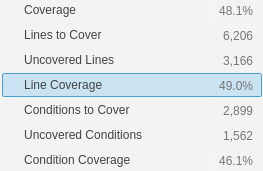
\includegraphics[width=0.5\textwidth]{./Resources/cobertura_jacoco}
	\caption{Medida de cobertura do projeto obtida com o JaCoCo} 
	Fonte: Autor
	\label{fig:cobertura_jacoco}
\end{figure}

\par A cobertura dos testes por m�dulo s�o apresentadas nas figuras~\ref{fig:cobertura_modulo_android_studio} e~\ref{fig:cobertura_modulo_jacoco}. A partir destes dois gr�ficos apresentados, pode-se dizer que a medi��o realizada pelo Android Studio se mostra mais exata ao que foi feito, j� que as medidas do JaCoCo indicam uma cobertura de 0\% para a USART, quando existem 7 casos de teste para este m�dulo, e 100\% para m�dulo de E/S, quando n�o foi escrito nenhum caso de teste para este m�dulo, por este ser mais dedicado � opera��es com interface gr�fica.

\begin{figure}[h!]
	\centering
	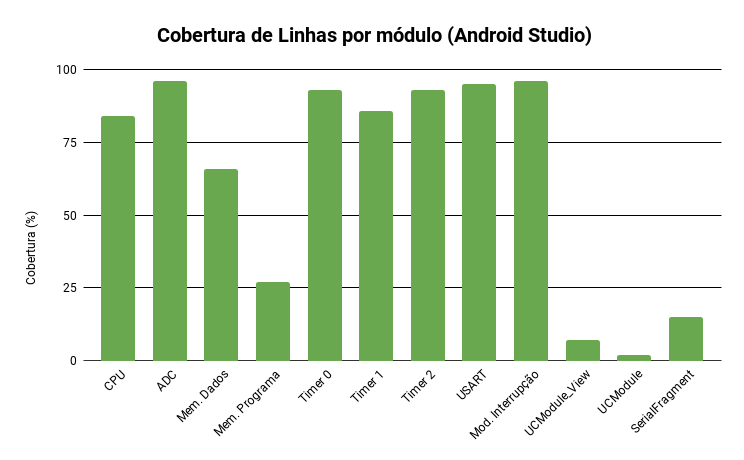
\includegraphics[width=\textwidth]{./Resources/cobertura_modulo_android_studio}
	\caption{Cobertura por m�dulo (Android Studio)} 
	Fonte: Autor
	\label{fig:cobertura_modulo_android_studio}
\end{figure}

\begin{figure}[h!]
	\centering
	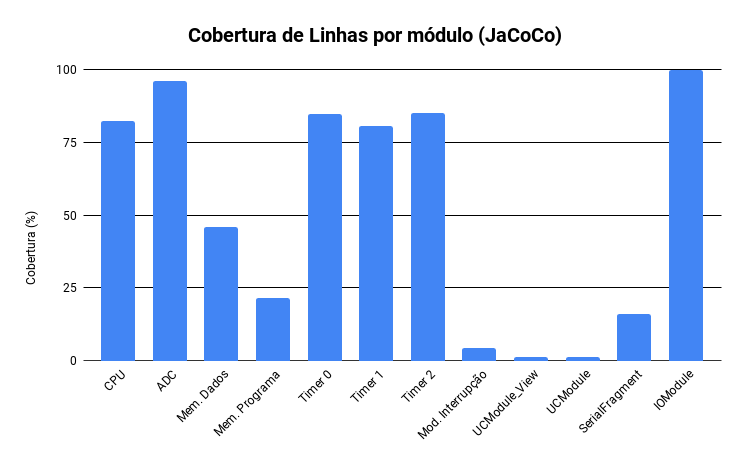
\includegraphics[width=\textwidth]{./Resources/cobertura_modulo_jacoco}
	\caption{Cobertura por m�dulo (JaCoCo)} 
	Fonte: Autor
	\label{fig:cobertura_modulo_jacoco}
\end{figure}

\par Al�m dos testes automatizados, foram realizados testes manuais das funcionalidades desenvolvidas. Todos os c�digos testados podem ser vistos na se��o de ap�ndice deste trabalho.

\section{\textit{Profiling}}
\label{profiling}

\par Foi utilizada a ferramenta de \textit{profilling} do pr�prio Android Studio para avaliar o consumo de recursos do aplicativo e tentar identificar pontos de otimiza��o. O projeto \textit{Blink} (ap�ndice~\ref{apendice_blink}), foi utilizado no simulador durante a execu��o do \textit{profilling}. 
\par O sistema foi avaliado quanto ao seu uso de CPU e mem�ria, a figura~\ref{fig:profilling_geral} mostra o desempenho do sistema considerando estes dois fatores. Pode-se observar que o uso de CPU fica em torno de 25\%, enquanto que o uso de mem�ria � de aproximadamente 30MB.

\begin{figure}[H]
	\centering
	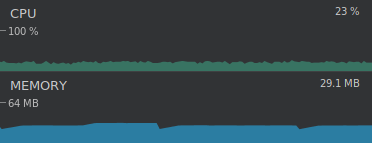
\includegraphics[width=0.75\textwidth]{./Resources/profilling_general}
	\caption{Uso de CPU e mem�ria para o projeto \textit{Blink}} 
	Fonte: Autor
	\label{fig:profilling_geral}
\end{figure} 

\par Olhando especificamente para a CPU (utilizando a op��o de grava��o instrumentada para rastreamento de m�todos), observou-se que muito do uso de CPU n�o est� relacionado diretamente com as classes desenvolvidas, mas sim com chamadas � classes internas do Android. Do que foi desenvolvido, a classe \textit{UCModule\_View} se mostrou o principal ponto cr�tico, mais especificamente o m�todo \textit{run}, que faz a atualiza��o do tempo simulado na tela. A figura~\ref{fig:profilling_cpu} apresenta este resultado.

\begin{figure}[h]
	\centering
	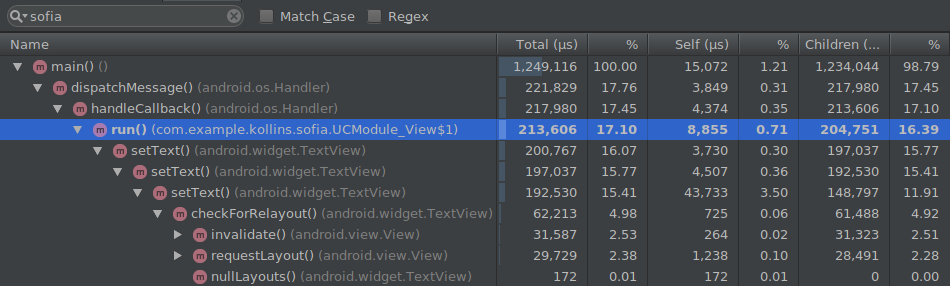
\includegraphics[width=\textwidth]{./Resources/profilling_cpu}
	\caption{Tempo de uso da CPU (medido em uma janela de 5 minutos)} 
	Fonte: Autor
	\label{fig:profilling_cpu}
\end{figure} 

\par Uma medida tomada quanto � este resultado foi atrasar a atualiza��o do tempo simulado por um fator de 1024, ou seja, uma requisi��o de atualiza��o da tela s� � dada ap�s 1024 passagens pelo m�todo \textit{run}. O valor de 1024 foi obtido experimentalmente de modo a n�o prejudicar a fluidez da interface (valores maiores fazem com que o tempo simulado salte de um valor para outro, dando a impress�o que o sistema est� a ponto de travar).
\par Essa medida teve um impacto significativo no desempenho deste m�todo, que passou de um uso de CPU em torno de 17\% para pouco menos de 0,5\% , como mostra a figura~\ref{fig:profilling_cpu_melhoria}.

\begin{figure}[H]
	\centering
	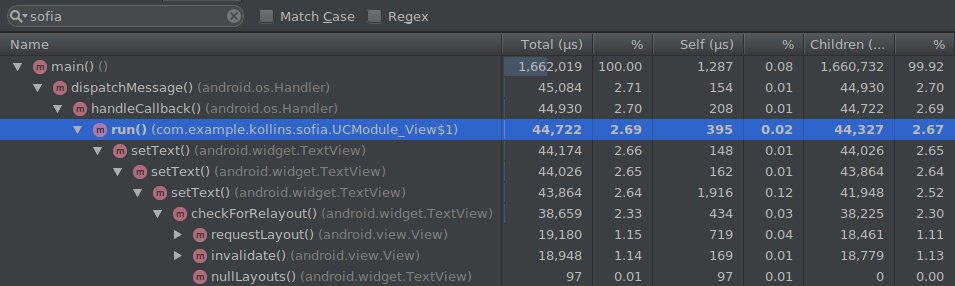
\includegraphics[width=\textwidth]{./Resources/profilling_cpu_melhoria}
	\caption{Tempo de uso da CPU ap�s melhoria no m�todo \textit{run} (medido em uma janela de 5 minutos)} 
	Fonte: Autor
	\label{fig:profilling_cpu_melhoria}
\end{figure} 

\hfil
\par Tamb�m foi feito um \textit{profilling} espec�fico para o uso de mem�ria. Os resultados s�o mostrados na figura~\ref{fig:profilling_memoria}.

\begin{figure}[h]
	\centering
	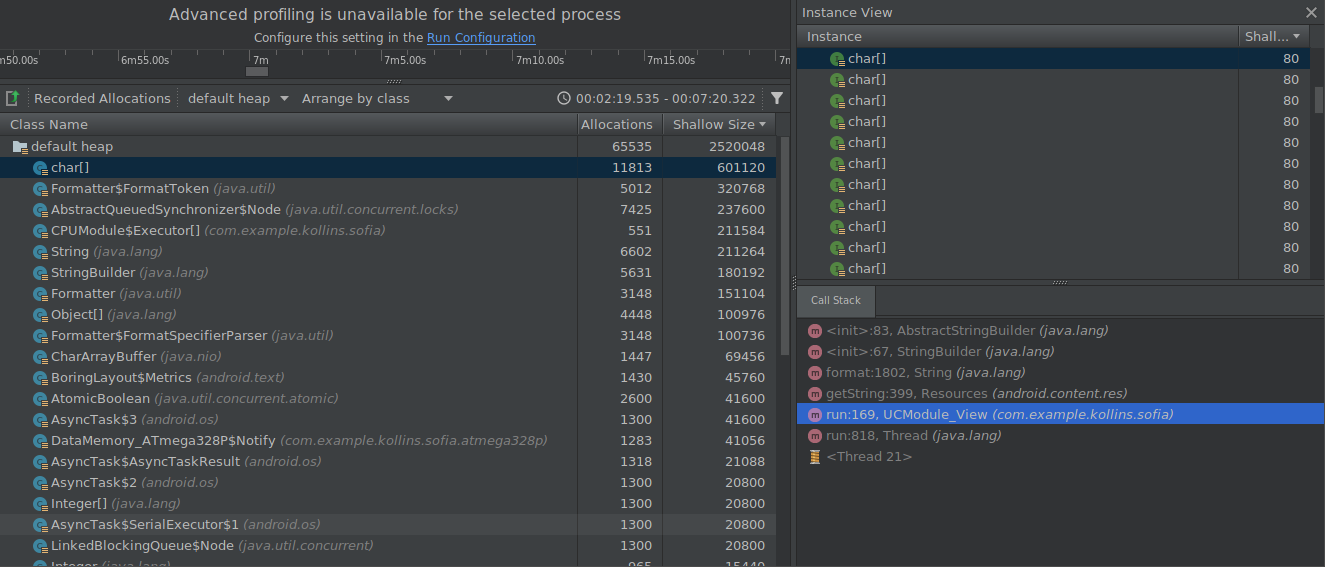
\includegraphics[width=\textwidth]{./Resources/profilling_memoria}
	\caption{Consumo de mem�ria (medido em uma janela de 5 minutos)} 
	Fonte: Autor
	\label{fig:profilling_memoria}
\end{figure} 

\par O que se observa em termos de mem�ria � que as estruturas de \textit{Enum}, utilizadas na CPU e nos temporizadores, foram as respons�veis por fazer com que estes m�dulos se destacassem no uso de mem�ria. De certa forma, este resultado j� era esperado uma vez que estas s�o estruturas est�ticas, o que demanda um maior tamanho em mem�ria e n�o s�o limpas pelo \textit{Garbage Collector} do Java.

\par Por outro lado, o uso de \textit{Enum} permitiu obter uma funcionalidade pr�xima aos ponteiros de fun��o que se tem na linguagem C, recurso bastante �til para fazer a decodifica��o das instru��es na CPU (bem como a sele��o do \textit{prescaler} nos temporizadores). 

\par Como mencionado na se��o~\ref{teoria_cpu}, manter a legibilidade do c�digo durante a decodifica��o foi uma grande preocupa��o durante o desenvolvimento. O uso de mem�ria � um pre�o a se pagar por essa facilidade obtida com a estrutura \textit{Enum}. Mesmo assim, o aplicativo n�o apresenta valores elevados de consumo de mem�ria quando comparado com outros aplicativos semelhantes, como mostra a se��o~\ref{sec:comparacao}.

\section{Compara��o entre aplicativos}
\label{sec:comparacao}

\par Foram 3 os aplicativos selecionados para serem comparados com o projeto SOFIA, s�o eles:

\begin{itemize}
	\item \textit{Arduino Simulator Mini Free}
	\item \textit{BoardMicro - AVR Simulator} (aplicativo e \textit{web}).
	\item \textit{AndMCU} (ou \textit{MCU Prototype Board Simulator})
\end{itemize}

\par Os aplicativos n�o s�o exatamente uma alternativa uns dos outros, mas apresentam caracter�sticas semelhantes e um mesmo prop�sito, que � a simula��o de um microcontrolador.

%\par Apesar de o aplicativo \textit{AndMCU} n�o estar diretamente relacionado com Arduino ou a arquitetura AVR, seu prop�sito � basicamente o mesmo do proposto que � proposto neste trabalho e portanto decidiu-se por analis�-lo tamb�m.

\par Para a realiza��o dos testes, foi utilizado novamente o projeto \textit{Blink} do ap�ndice~\ref{apendice_blink} nos simuladores \textit{BoardMicro - AVR Simulator} e SOFIA. O aplicativo \textit{Arduino Simulator Mini Free} n�o permite a edi��o de c�digos, mas possui o mesmo projeto dispon�vel para simula��o. Quanto ao \textit{AndMCU}, foi escrito um programa em \textit{assembly} mostrado no ap�ndice~\ref{apendice_blink_asm} para a poder test�-lo, j� que este simulador se destina � outra plataforma. 

\par O aparelho utilizado em todos os testes foi um \textit{smartphone} ASUS ZenFone 2, com 4 n�cleos de processamento (2,33GHz), 4GB de mem�ria principal e 32GB de armazenamento, executando o Android 5.0.

\subsection{Interface}

\par O primeiro ponto a ser comparado s�o as interfaces que cada aplicativo oferece para ao usu�rio.

\par O projeto SOFIA, como j� foi mostrado na se��o~\ref{resultado_sofia}, procura oferecer uma interface simples, sem fazer refer�ncia � componentes eletr�nicos. Na tela principal, o usu�rio tem sempre a sua disposi��o bot�es para realizar todas as tarefas que desejar no aplicativo, seja inserir novos elementos, reiniciar a simula��o ou acessar fun��es adicionais, tudo isso sem que seja necess�rio acessar novas telas. A figura~\ref{fig:interface_sofia} mostra a interface principal da SOFIA com algumas entradas e sa�das.

\begin{figure}[h]
	\centering
	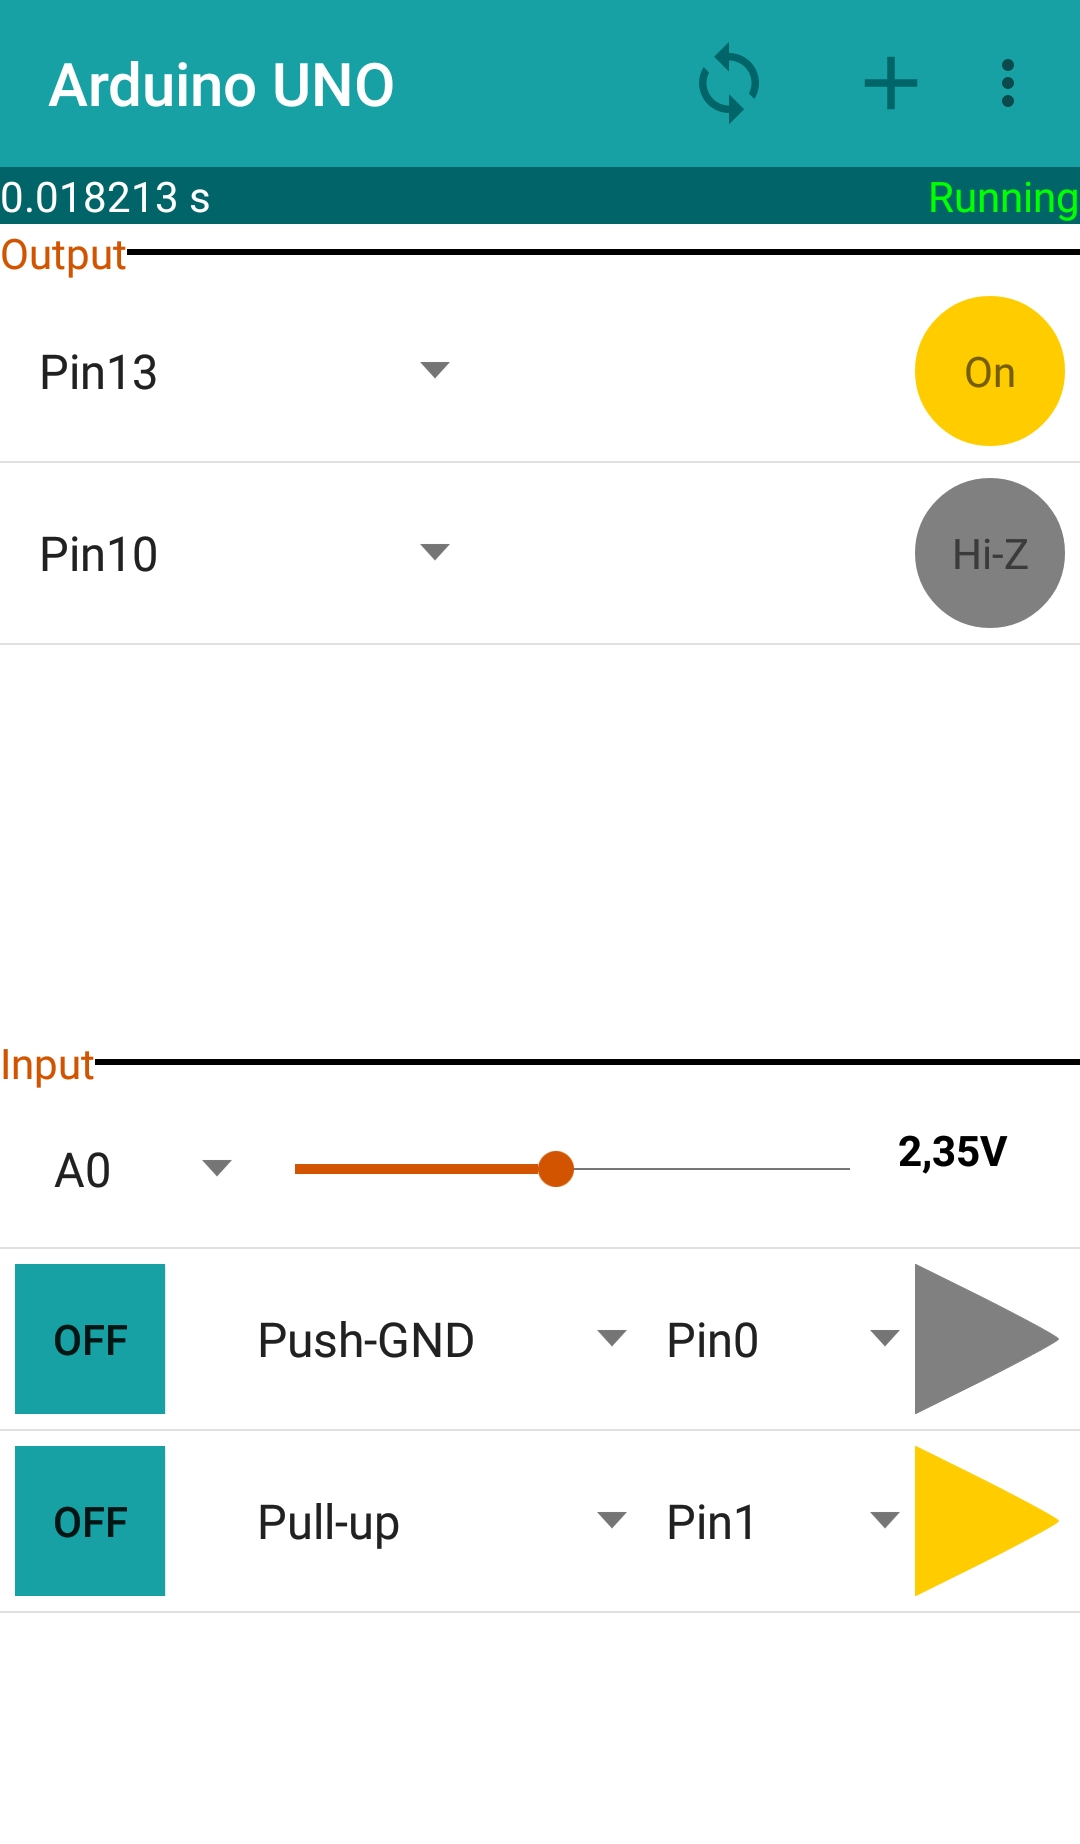
\includegraphics[scale=0.70]{./Resources/simulation_with_io}
	\caption{Tela principal do simulador SOFIA} 
	Fonte: Autor
	\label{fig:interface_sofia}
\end{figure} 

\par Uma desvantagem desta interface � que ela n�o � t�o intuitiva aos usu�rios, que poder�o levar algum tempo para se acostumar, principalmente aqueles que procuram por refer�ncias visuais dos componentes eletr�nicos, como LEDs, \textit{protoboards}, etc. Por este motivo, um bot�o de ajuda foi adicionado no aplicativo para levar o usu�rio � p�gina do projeto, onde ele ter� todas as informa��es necess�rias para o uso do simulador.

\par Al�m disso, o tamanho da tela � reduzido, de forma que a inser��o de muitos elementos pode prejudicar a experi�ncia do usu�rio em termos de visualiza��o dos resultados, j� que apenas parte das entradas/sa�das estar�o vis�veis (sem contar o poss�vel uso do monitor serial).

\par O simulador \textit{BoardMicro - AVR Simulator}, assim como no projeto SOFIA, tamb�m utiliza uma representa��o abstrata do sistema a ser simulado, como mostra a figura~\ref{fig:interface_BM_AVR}.

\begin{figure}[h]
	\centering
	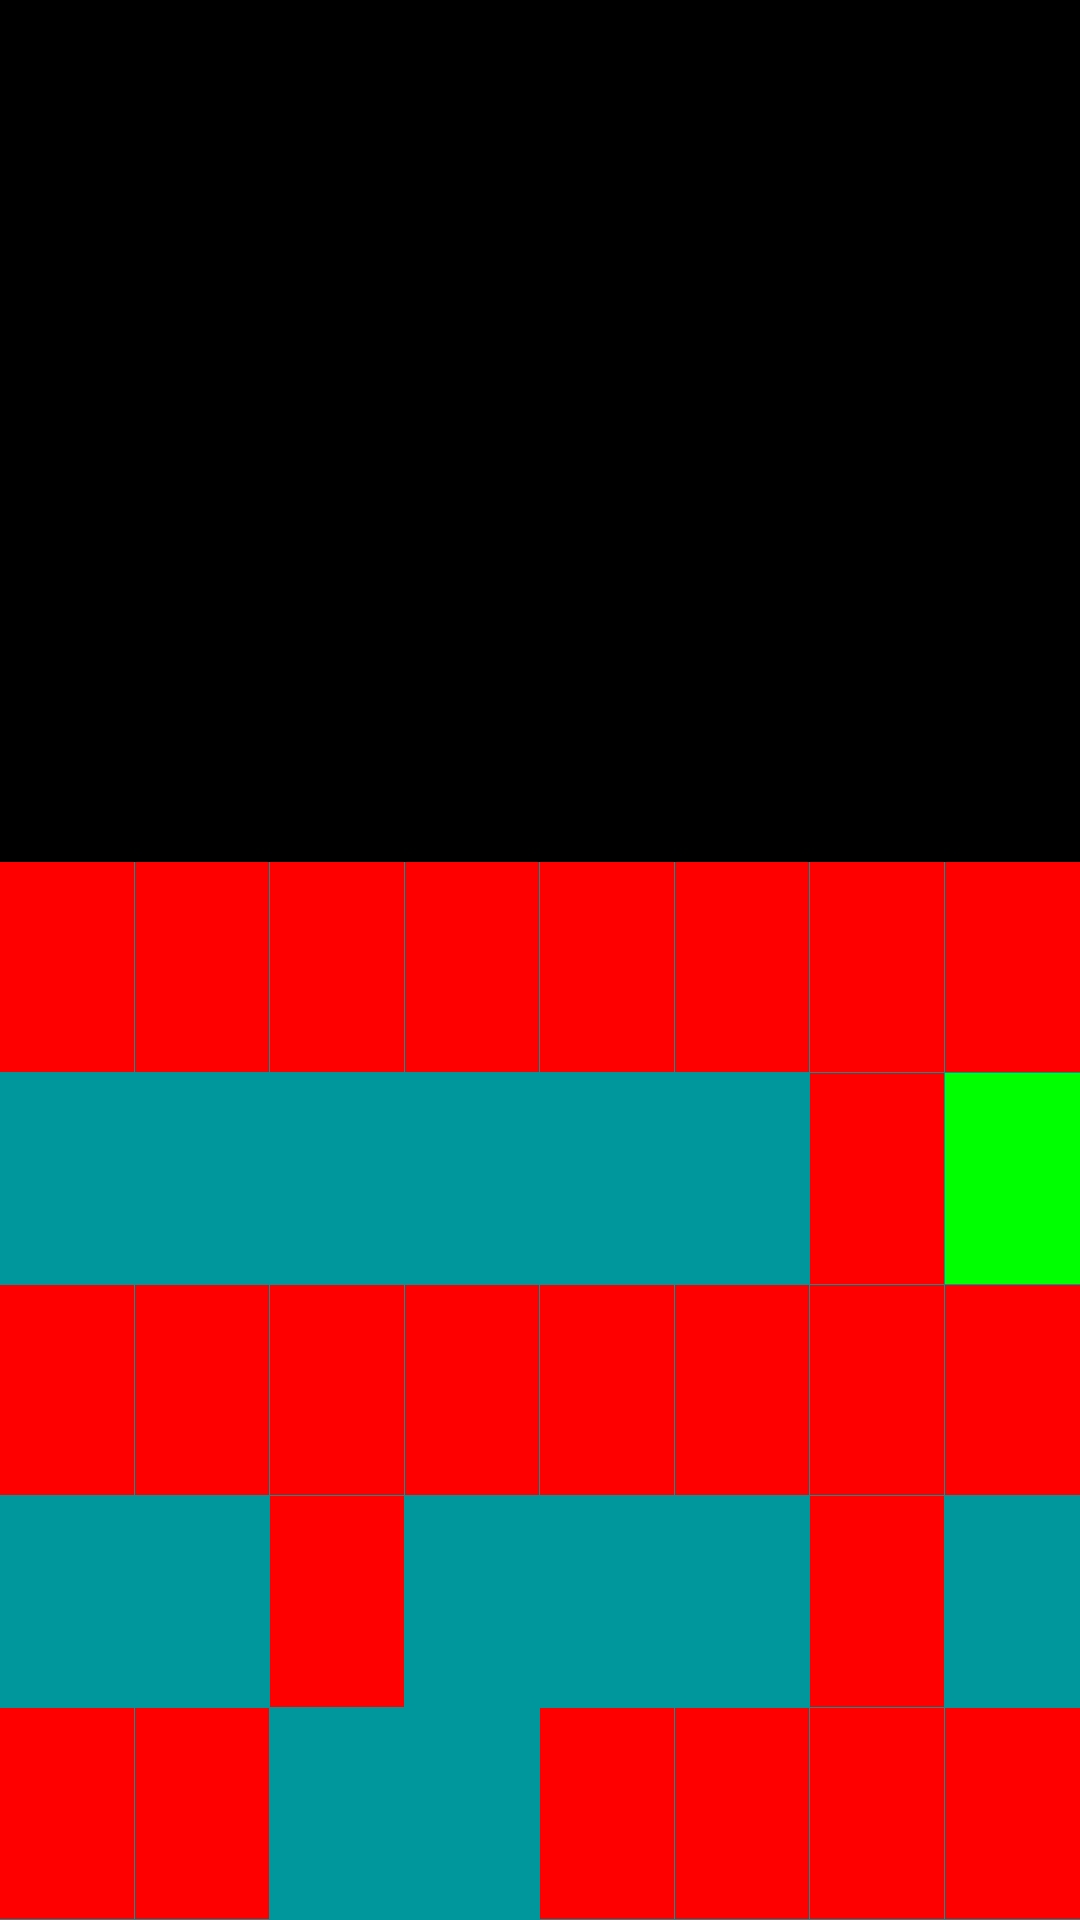
\includegraphics[scale=0.13]{./Resources/interface_BM_AVR}
	\caption{Tela principal do simulador \textit{BoardMicro - AVR Simulator}} 
	Fonte: Autor
	\label{fig:interface_BM_AVR}
\end{figure} 

\par Na tela principal, apenas est�o presentes a visualiza��o de uma tela TFT LCD na parte superior e dos PORTs de B a F (de cima para baixo). Na figura~\ref{fig:interface_BM_AVR}, a parte destacada em verde � o PORTC7, onde est� ligado o LED interno do Arduino Esplora.

\par N�o h� bot�es nem outras telas no aplicativo e toda a navega��o � feita por toques. Esta caracter�stica torna o sistema bastante dif�cil de se utilizar, principalmente por n�o haver uma ajuda indicando quais s�o as a��es poss�veis. Este simulador possui ainda uma vers�o \textit{web}, com uma interface ligeiramente diferente, com mais indica��es, como mostra a figura~\ref{fig:interface_BM_AVR_web}, o que facilita seu uso.

\begin{figure}[h!]
	\centering
	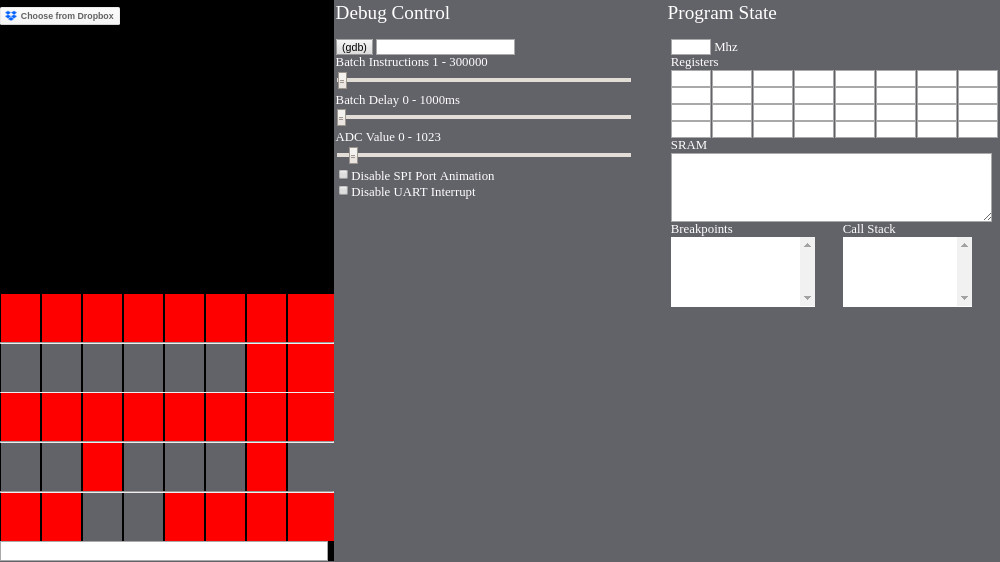
\includegraphics[width=\textwidth]{./Resources/interface_BM_AVR_web}
	\caption{Tela principal do simulador \textit{BoardMicro - AVR Simulator}, vers�o para \textit{web}} 
	Fonte: Autor
	\label{fig:interface_BM_AVR_web}
\end{figure} 

\par Esta escolha de interface se justifica uma vez que a plataforma alvo deste simulador � o Arduino Esplora, que possui a forma de um \textit{joystick} e pode ser conectado � um display externo (internamente, a tela TFT mostrada na parte superior est� interligada nos pinos de comunica��o SPI do ATmega32U4 para estabelecer esta conex�o). Mesmo assim, a falta completa de informa��es/indica��es para o usu�rio dificultam o entendimento do sistema, for�ando o usu�rio a estudar o aplicativo por algum tempo antes de poder utiliz�-lo.

\newpage

\par Partindo para o \textit{AndMCU}, este possui uma interface que lembra um kit de desenvolvimento PIC, mostrando inclusive o microcontrolador PIC18F458 (apesar do projeto funcionar com c�digos assembly do microcontrolador 68705 da Motorola). A interface deste simulador � mostrada na figura~\ref{fig:interface_AndMCU}.

\begin{figure}[h]
	\centering
	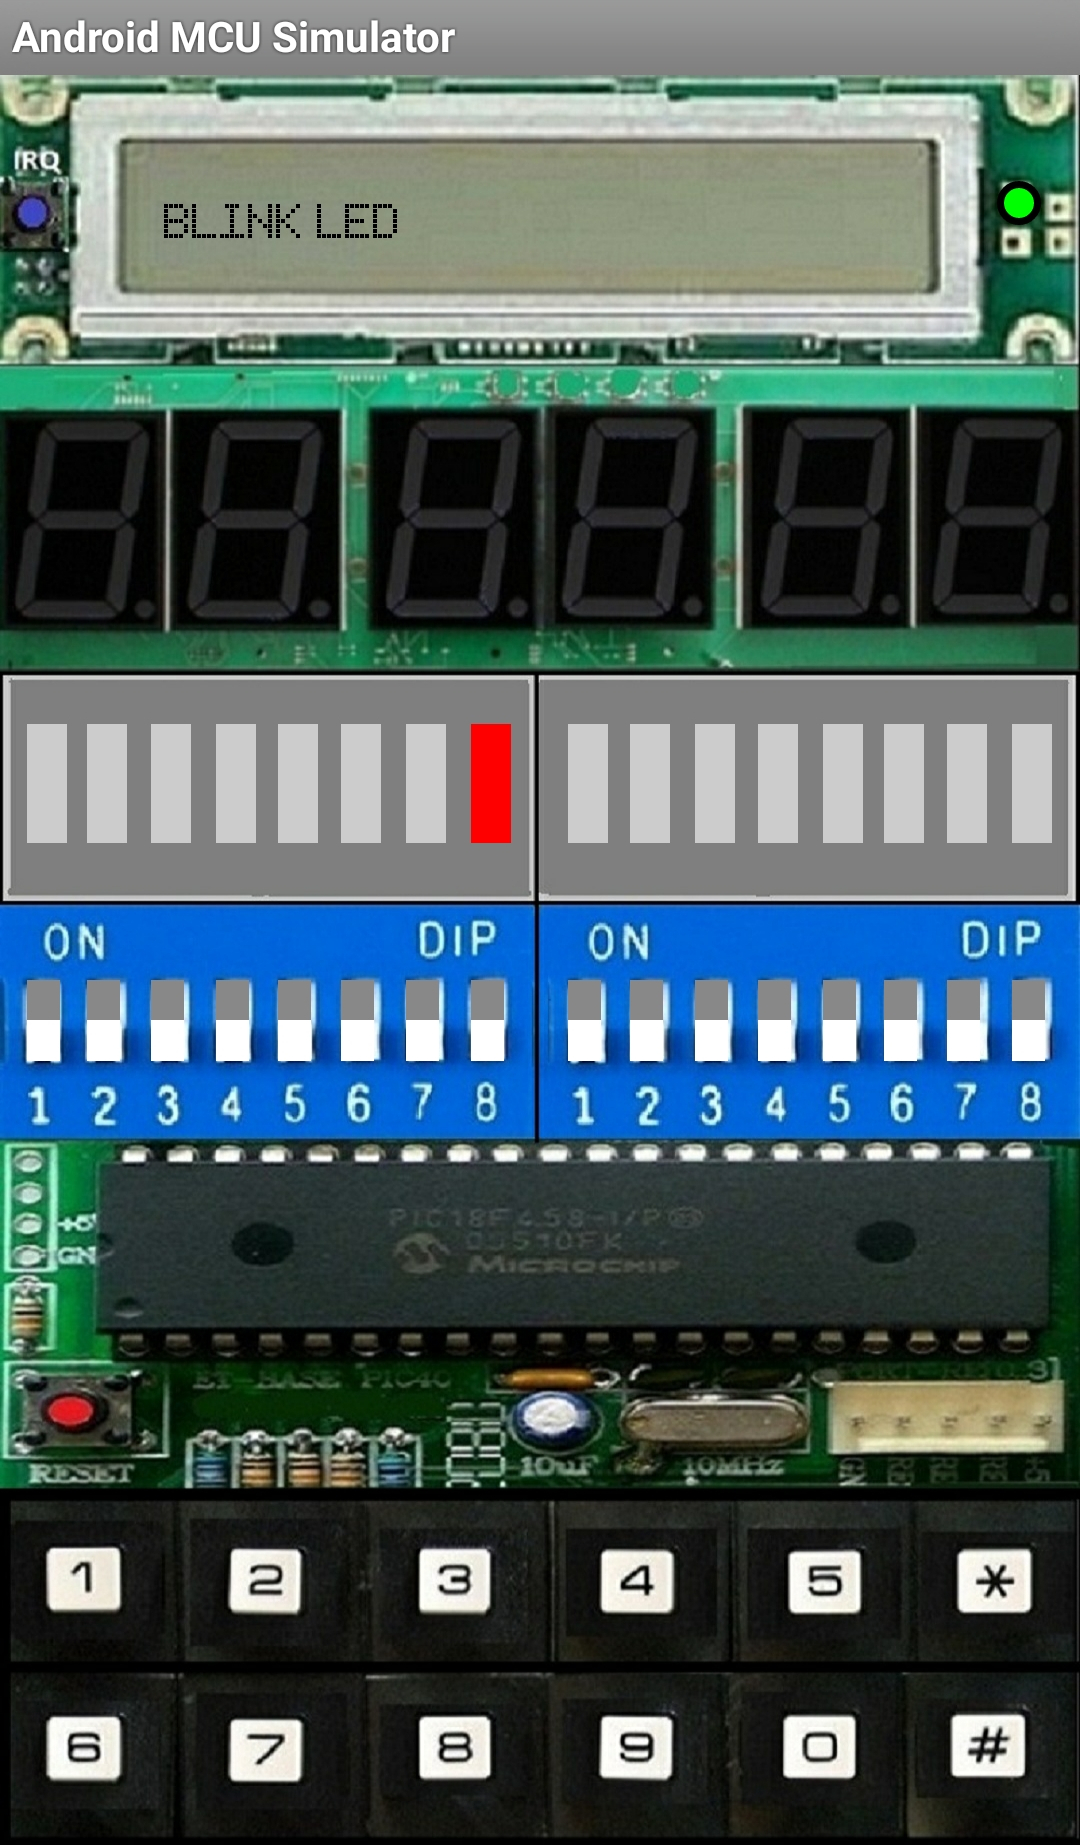
\includegraphics[scale=0.75]{./Resources/interface_AndMCU}
	\caption{Tela principal do simulador \textit{AndMCU}} 
	Fonte: Autor
	\label{fig:interface_AndMCU}
\end{figure} 

\par O kit apresentado conta com um display LCD de 16 caracteres, 6 displays de 7 segmentos, 2 barras gr�ficas com 8 LEDs cada, 2 \textit{DIP Switchs} de 8 vias e um teclado num�rico. Al�m disso, existe um bot�o azul no canto superior esquerdo para interrup��es externas, um bot�o vermelho para \textit{reset} manual no canto inferior esquerdo e um LED de status no canto superior direito. Tamb�m, o sistema utiliza o sensor de luminosidade do \textit{smartphone} como entrada anal�gica e a documenta��o do projeto menciona ainda um piezo \textit{buffer}~\cite{AndMCU}.

\par Este simulador tamb�m n�o conta com menus de ajuda ou qualquer instru��o de uso no aplicativo. Na verdade, uma vez escolhido o c�digo a ser executado, n�o h� mais nada a se fazer no simulador a n�o ser trabalhar em cima da simula��o atual. A troca de arquivos para simula��o exige sair do aplicativo e inici�-lo novamente.

\par Apesar disso, o \textit{AndMCU} apresenta um visual compacto, com boa disposi��o dos elementos na tela e com diversos recursos que devem ser facilmente reconhecidos por usu�rios j� experientes com microcontroladores e eletr�nica. O \textit{hardware} integrado d� a possibilidade para que o usu�rio possa testar os programas mais comuns e mesmo alguns mais avan�ados.

\par Por fim, o \textit{Arduino Simulator Mini Free} tamb�m prefere um visual mais realista do \textit{hardware}, como mostra a figura~\ref{fig:interface_ASMF}.

\begin{figure}[H]
	\centering
	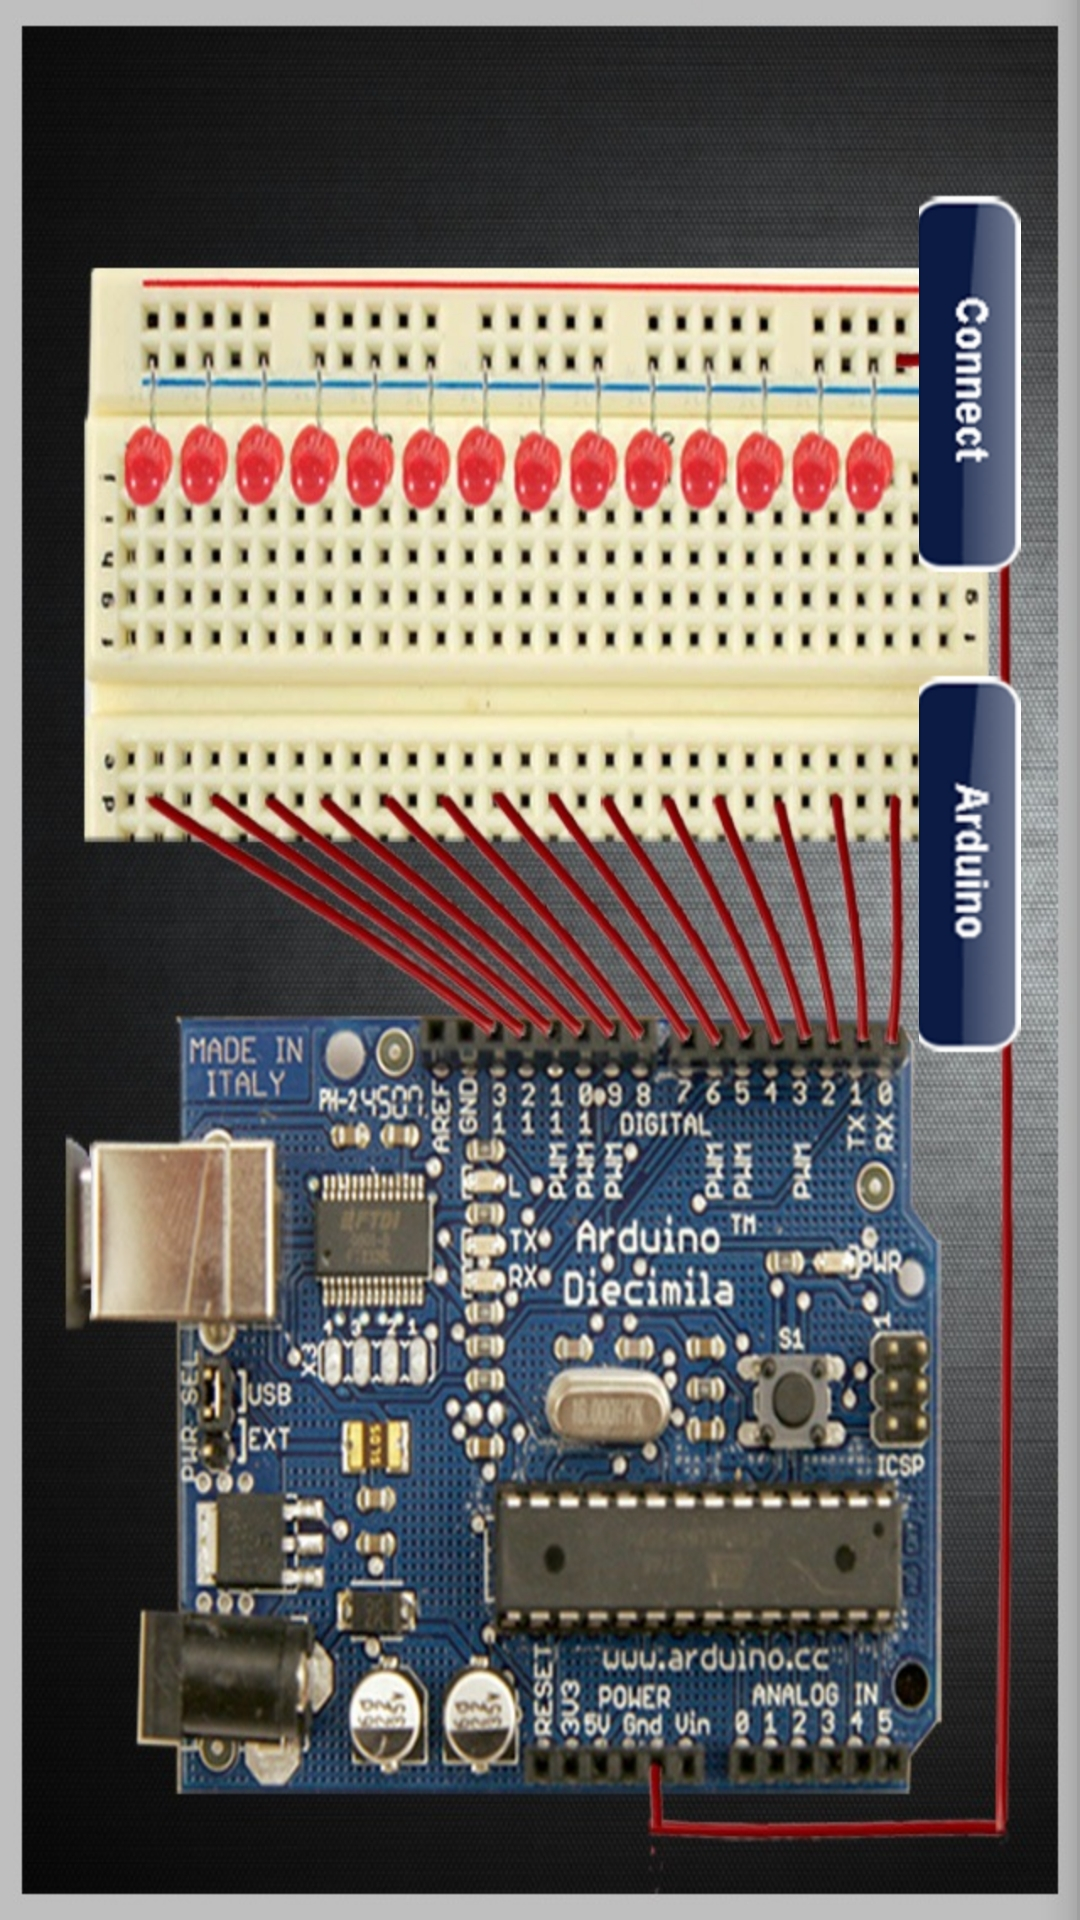
\includegraphics[scale=0.21,angle=90]{./Resources/interface_AMSF}
	\caption{Tela principal do simulador \textit{Arduino Simulator Mini Free}} 
	Fonte: Autor
	\label{fig:interface_ASMF}
\end{figure} 

\par Durante a simula��o, o circuito � alterado no \textit{protoboard} de forma a fornecer o \textit{hardware} adequado para simular o c�digo. A figura~\ref{fig:interface_ASMF_blink} mostra a interface para simula��o do projeto \textit{Blink}.

\begin{figure}[h]
	\centering
	\includegraphics[scale=0.21,angle=90]{./Resources/interface_AMSF_blink}
	\caption{Tela de simula��o do projeto \textit{Blink}. O monitor serial no canto inferior direito pode ser escondido por meio do bot�o "\textit{Console}"} 
	Fonte: Autor
	\label{fig:interface_ASMF_blink}
\end{figure} 

\par Tamb�m para a visualiza��o do c�digo, o simulador busca uma interface que lembra a IDE do Arduino, como mostra a figura~\ref{fig:interface_ASMF_IDE}.

\begin{figure}[h]
	\centering
	\includegraphics[scale=0.21,angle=90]{./Resources/interface_AMSF_IDE}
	\caption{Tela edi��o do c�digo fonte a ser simulado.} 
	Fonte: Autor
	\label{fig:interface_ASMF_IDE}
\end{figure} 

\par O realismo buscado pelo \textit{Arduino Simulator Mini Free} pode ajudar o usu�rio que deseja, al�m de realizar a simula��o, fazer a montagem posterior do circuito, j� que o simulador mostra todo o esquem�tico necess�rio para executar o projeto.

\par Al�m disso, o \textit{design} proposto minimiza as d�vidas quanto ao seu uso. Ainda que n�o haja instru��es, os elementos utilizados s�o bem conhecidos daqueles que j� utilizam a IDE do Arduino e os bot�es possuem identificadores bastante claros quanto sua fun��o, de modo que, muito provavelmente, apenas um usu�rio iniciante pode vir a ter alguma dificuldade em utilizar este aplicativo.

\subsection{Funcionalidades oferecidas}

\par Cada aplicativo oferece um conjunto de funcionalidades e possibilidades de uso diferentes para o usu�rio.

\par O projeto SOFIA � focado na simula��o do Arduino UNO e procura fornecer ao usu�rio um conjunto de ferramentas para que se possa, al�m de simular o funcionamento do c�digo, obter informa��es a respeito de sua execu��o. Desta forma, o sistema oferece a possibilidade de medi��o de frequ�ncia, \textit{duty cicle}, mem�ria, al�m de permitir a configura��o manual de uma refer�ncia externa de tens�o para o conversor A/D. Tamb�m, o monitor serial integrado d� ao usu�rio uma maior possibilidade na depura��o do c�digo, permitindo o envio de mensagens de dentro do c�digo para visualiza��o externa.
\par Al�m disso, o projeto SOFIA busca ser um simulador gen�rico, permitindo que o usu�rio entre com qualquer c�digo hexadecimal gerado, independente de sua fonte. O usu�rio tamb�m � livre para testar diversas possibilidades de liga��o entre entradas e sa�das, podendo mesmo interligar m�ltiplas entradas em um mesmo pino; ligar uma entrada anal�gica em um pino digital e ver o efeito que n�veis indefinidos de tens�o podem gerar; conta com aviso em caso de curto-circuito, etc. A ideia principal � que, apesar de ser um simulador, as possibilidades de uso se aproximem do que o usu�rio encontrar� em uma montagem eletr�nica real.

\par J� o projeto \textit{BoardMicro - AVR Simulator} � mais focado no uso do display TFT, fazendo com que o usu�rio explore este recurso para obter resultados de sua simula��o, j� que apenas a visualiza��o dos PORTs pode n�o ser o suficiente para obter informa��es.

\par Para intera��o com a simula��o, o simulador utiliza a leitura do aceler�metro do \textit{smartphone} como entrada anal�gica e permite tamb�m o envio de comandos do GDB (apesar desta op��o n�o funcionar no aplicativo). A vers�o \textit{web} permite ainda a medi��o de par�metros como o estado dos registradores, pilha, SDRAM e a velocidade do sistema, tamb�m permitindo controlar a velocidade de simula��o.

\par Como dito anteriormente, o aplicativo n�o possui bot�es ou menus e a navega��o por toques n�o � clara, mas � por meio dela � poss�vel abrir o menu para carregar um c�digo hexadecimal e acessar o \textit{prompt} do GDB. Um programa a ser simulado pode tanto ser escolhido de um banco de exemplos (com 4 c�digos dispon�veis no aplicativo) ou carregados pelo usu�rio a partir de um reposit�rio do Dropbox.

\par O \textit{AndMCU} fornece um kit de desenvolvimento ao usu�rio e as possibilidades de intera��o com o aplicativo n�o vai muito al�m das possibilidades deste \textit{hardware} virtual (com exce��o para o uso do sensor de luminosidade do \textit{smartphone} para entrada anal�gica). A �nica intera��o do usu�rio que � externo � este kit � na escolha do c�digo a ser simulado ao iniciar o aplicativo.

\par Apesar disso, o sistema permite que diversas configura��es sejam feitas no c�digo em \textit{assembly} que ser� simulado. Entre as possibilidades est�o o controle de velocidade de simula��o, modo de simula��o passo-a-passo, desabilitar os \textit{DIP Switches}, escrever conte�do da mem�ria em arquivo, entre outras possibilidades descritas na documenta��o.

\par O simulador fornece, assim como o \textit{BoardMicro - AVR Simulator}, um banco contendo 10 exemplos j� codificados e um arquivo \textit{template} para servir de base para novos c�digos. O usu�rio que desejar simular um c�digo diferente deve adicion�-lo na pasta \url{/sdcard/AndMCU} do \textit{smartphone}.

\par E finalmente, o \textit{Arduino Simulator Mini Free} se mostrou-se o mais limitado em temos de funcionalidade. O simulador fornece 5 c�digos exemplo para o usu�rio, que pode realizar modifica��es apenas de determinados par�metros, como alterar o pino de sa�da, tempo de \textit{delay} e mensagem do display LCD, n�o sendo poss�vel criar um c�digo customizado para a simula��o. 
\par O usu�rio tamb�m n�o pode fornecer dados de entrada durante a simula��o, podendo apenas visualizar o funcionamento do circuito. Isso acaba invalidando um dos c�digos exemplo, que requer uma entrada anal�gica em um circuito utilizando LDR.
\par O \textit{Arduino Simulator Mini Free} possui duas outras vers�es pagas na \textit{Amazon Store}, com diferentes projetos e a possibilidade de edi��o do circuito eletr�nico em uma delas (segundo a descri��o). No entanto, nenhuma destas vers�es foi testada.

\subsection{Requisitos do sistema e consumo de recursos}

\subsubsection{Sistema Operacional}

\par Todos os aplicativos suportam o sistema Android, com o \textit{Arduino Simulator Mini Free} dispon�vel tamb�m para IOs (sob os nomes \textit{Arduino Simulator 2X - Learn and DIY Safely} e \textit{Arduino Simulator - Full Pack 2x}). A tabela~\ref{tab:comp_plataforma} indica qual a vers�o m�nima do Android � requerida por cada aplicativo. Este valor foi obtido a partir da descri��o do aplicativo nas lojas \textit{Google Play Store} e \textit{Amazon Store}.

\begin{table}[h]
	\centering
	\caption{Vers�o do Android requerida por cada aplicativo}
	\label{tab:comp_plataforma}
	\begin{tabular}{|c|c|}
		\hline
		\textbf{Aplicativo} & \textbf{Vers�o do m�nima} \\ \hline
		Arduino Simulator Mini Free & 2.2 \\ \hline
		AndMCU & 2.3.3 \\ \hline
		BoardMicro - AVR Simulator & 4.0 \\ \hline		
		SOFIA & 5.0 \\ \hline
	\end{tabular}
\end{table}

\par Ao criar um projeto no Android Studio, pode-se verificar qual a distribui��o de usu�rios em cada vers�o do Android. A figura~\ref{fig:dist_android} apresenta esta distribui��o e por ela, pode-se observar que, com exce��o do projeto SOFIA, todos os simuladores podem ser executados em 100\% dos dispositivos Android ativos no momento.

\begin{figure}[h!]
	\centering
	\includegraphics[width=0.45\textwidth]{./Resources/distrib_android}
	\caption{Distribui��o acumulada de usu�rios Android. Como destacado, o simulador SOFIA poder� atingir pouco mais de 70\% dos dispositivos Android ativos no momento, por�m este n�mero tente a aumentar com a moderniza��o dos aparelhos} 
	Fonte: Android Studio
	\label{fig:dist_android}
\end{figure}

\subsubsection{Tamanho}

\par O gr�fico mostrado na figura~\ref{fig:comp_tamanho} mostra o tamanho do arquivo APK para cada aplicativo.

\begin{figure}[h!]
	\centering
	\includegraphics[width=\textwidth]{./Resources/tamanho_apk}
	\caption{Tamanho do arquivo APK (MB) de cada aplicativo} 
	Fonte: Autor
	\label{fig:comp_tamanho}
\end{figure} 

\par Pode-se observar que o \textit{Arduino Simulator Mini Free} possui um tamanho muito superior aos demais, resultado este um tanto inesperado, uma vez que a vers�o \textit{Full Pack} deste aplicativo possui um tamanho menor de apenas 9MB.

\newpage
\subsubsection{Uso de CPU}

\par O uso de CPU foi medido utilizando um \textit{shell} remoto acessado pelo \textit{Android Debug Bridge} (adb). O comando \textit{top} pode ser utilizado de modo an�logo ao \textit{htop} dos sistemas Linux, e mostra diversas informa��es a respeito dos processos em execu��o, incluindo o uso de CPU. O gr�fico da figura~\ref{fig:comp_cpu} apresenta a m�dia obtida das medi��es, com indica��o do desvio padr�o. O aplicativo \textit{AndMCU} foi testado em duas condi��es diferentes, para alta e baixa velocidade de simula��o, definida pela diretriz \textit{.speed}.

\begin{figure}[h!]
	\centering
	\includegraphics[width=\textwidth]{./Resources/uso_cpu}
	\caption{Consumo m�dio de CPU (\%) de cada aplicativo. Para cada processo, foram coletadas 397 amostras} 
	Fonte: Autor
	\label{fig:comp_cpu}
\end{figure} 

\par � dif�cil comparar o resultado do \textit{AndMCU} com os demais aplicativos pois, em todos eles, o c�digo foi o mesmo (em C), a plataforma � a mesma (Arduino) e a frequ�ncia de intermit�ncia � a mesma (500Hz), enquanto que o \textit{AndMCU} est� em outro contexto, com c�digo em \textit{assembly}, produzindo uma frequ�ncia de intermit�ncia dif�cil de ser determinada. O que se observou, no entanto, foi que este aplicativo apresentou um consumo de CPU bastante reduzido em compara��o aos demais, mesmo quando a velocidade de simula��o foi configurada para a m�xima poss�vel.

\par Por outro lado, o simulador \textit{BoardMicro - AVR Simulator} apresentou um consumo muito maior que a m�dia dos demais, resultado este que provavelmente est� relacionado com sua velocidade de simula��o, como mostra a se��o~\ref{velocidade_simulacao}, enquanto o projeto SOFIA e o \textit{Arduino Simulator Mini Free} apresentaram resultados pr�ximos da m�dia.

\newpage

\par Esta medida de CPU tem impacto direto no consumo de bateria de cada aplicativo. A figura~\ref{fig:comp_bateria} apresenta um gr�fico indicando o consumo m�dio percentual de bateria para cada aplicativo em um per�odo de 2 horas, onde cada aplicativo ficou em execu��o cont�nua durante 30 minutos (o aplicativo \textit{AndMCU} foi utilizado em seu modo padr�o, ou seja, baixa velocidade). Os resultados foram medidos com a ferramenta \textit{Battery Historian} e pode-se observar que o gr�fico apresenta as mesmas propor��es ao apresentado na figura~\ref{fig:comp_cpu}.

\begin{figure}[h!]
	\centering
	\includegraphics[width=\textwidth]{./Resources/uso_bateria}
	\caption{Consumo m�dio de Bateria (\%) de cada aplicativo em um per�odo de 2 horas, com cada aplicativo executando o projeto \textit{Blink} continuamente por 30 minutos} 
	Fonte: Autor
	\label{fig:comp_bateria}
\end{figure} 

\subsubsection{Uso de Mem�ria}

\par O uso de mem�ria por cada aplicativo foi tamb�m medido do o uso do \textit{shell} remoto, com o comando \textit{dumpsys meminfo}. Segundo a documenta��o desta instru��o~\cite{Meminfo}, o campo \textit{Proportional Set Size} (PSS), que � a soma da mem�ria privada (regi�o de mem�ria pertencente apenas ao aplicativo e liberada ao sistema quando este � encerrado) e da mem�ria compartilhada (total de mem�ria compartilhada utilizada pelo aplicativo, dividida pelo n�mero de processos que compartilham a esta regi�o de mem�ria), fornece uma boa medida do "peso" deste processo na mem�ria principal, e portanto, este foi o valor utilizado para comparar o uso de mem�ria entre os aplicativos. O gr�fico da figura~\ref{fig:comp_ram} apresenta a m�dia obtida das medi��es realizadas, com indica��o do desvio padr�o.

\begin{figure}[h!]
	\centering
	\includegraphics[width=\textwidth]{./Resources/uso_ram}
	\caption{Consumo de mem�ria (PSS em MB) de cada aplicativo. Foram realizadas 1000 medi��es para cada aplicativo} 
	Fonte: Autor
	\label{fig:comp_ram}
\end{figure} 

\par No quesito mem�ria, embora o coment�rio a respeito do uso da estrutura \textit{Enum} na se��o~\ref{profiling}, o projeto SOFIA se mostrou bastante competitivo em rela��o aos demais simuladores.

\par Tamb�m foi interessante notar, no \textit{AndMCU}, que a configura��o de maior velocidade teve um consumo de mem�ria ligeiramente menor que o modo de baixa velocidade (apesar do grande desvio obtido). A explica��o para isso provavelmente se deve � taxa de atualiza��o da tela nos diferentes modos, como explicado na documenta��o~\cite{AndMCU}, o modo de alta velocidade diminui a taxa de atualiza��o e o oposto ocorre para o modo de baixa velocidade. Na se��o~\ref{profiling} foi mostrado que este par�metro tem grande impacto no consumo de CPU e de mem�ria no Android.

%\subsubsection{Consumo de Bateria}
%
%\par Por fim, foi realizada a medida do consumo de bateria dos aplicativos utilizando a ferramenta \textit{Battery Historian}. Cada aplicativo foi executado durante 5 minutos (com o projeto \textit{Blink}) e obteve-se o percentual de uso de bateria de cada aplicativo durante todo o per�odo de teste (aproximadamente 20 minutos). Este processo foi repetido tr�s vezes e o gr�fico da figura~\ref{fig:comp_bateria} apresenta a m�dia obtida. Pode-se observar que os dados est�o em concord�ncia com o gr�fico da figura~\ref{fig:comp_cpu}, como era de se esperar.
%
%\begin{figure}[h!]
%	\centering
%	\includegraphics[width=\textwidth]{./Resources/consumo_bateria}
%	\caption{Consumo percentual de bateria por cada aplicativo. Os demais recursos do sistema Android ficam respons�veis pelo percentual restante.} 
%	Fonte: Autor
%	\label{fig:comp_bateria}
%\end{figure} 
%
%\par Por n�o haver diferen�as significativas entre os modos de alta e baixa velocidade, o simulador \textit{AndMCU} foi testado em seu modo padr�o (baixa velocidade).

\subsection{Velocidade de simula��o}
\label{velocidade_simulacao}

\par A velocidade de simula��o aqui apresentada � uma medida da percep��o que o usu�rio tem do sistema, quando comparado com o tempo do mundo real.

\par Velocidade de simula��o provavelmente � a maior limita��o do projeto SOFIA. � poss�vel ter uma ideia clara desta velocidade uma vez � apresenta a contagem do tempo simulado para o usu�rio. Este tempo simulado est� reduzido em torno de 500x em compara��o com o tempo real, j� que s�o contados 2ms a cada segundo. Assim, o usu�rio percebe, na pr�tica, um sistema com frequ�ncia de \textit{clock} efetiva de 32kHz, uma vez que que o \textit{hardware} no qual o simulador se baseia � o Arduino UNO com frequ�ncia de 16MHz.

\newpage

\par Para os demais simuladores, a velocidade de simula��o foi medida alterando o projeto \textit{Blink} para que a intermit�ncia fosse de 1s. O \textit{Arduino Simulator Mini Free} se mostrou bastante fiel ao tempo real, exibindo, de fato, uma intermit�ncia de 1s, fazendo com que o usu�rio n�o perceba a diferen�a deste com um sistema real. J� o simulador \textit{BoardMicro - AVR Simulator} se mostra acelerado, com uma frequ�ncia  de intermit�ncia 4x maior que a esperada.

\par Para o projeto \textit{AndMCU}, n�o foi poss�vel ter uma ideia clara de sua real velocidade de simula��o pois, como j� mencionado anteriormente, este aplicativo est� em outro contexto do qual n�o � bem determinado/conhecido como no caso do Arduino. No entanto, � poss�vel ler na documenta��o do projeto que o sistema possui uma velocidade de simula��o adequada para que os resultados possam ser observados por estudantes, ou, como o autor coloca em outras palavras, "n�o se deve esperar deste simulador uma velocidade elevada como o de um emulador de CPU" (em tradu��o live)~\cite{AndMCU}.

\subsection{Documenta��o}

\par O projeto SOFIA conta com uma documenta��o \textit{on-line} (em ingl�s) hospedada no Gitbook. Esta documenta��o pode ser acessada a partir do reposit�rio do Github ou de dentro do pr�prio aplicativo, nos menus de ajuda e de informa��es do projeto.

\par A documenta��o do projeto SOFIA � dividido em 3 partes. A primeira mostra uma vis�o geral, apresentando uma breve descri��o do que � o projeto, seus objetivos, p�blico alvo, etc. A segunda parte � um manual do usu�rio e descreve, passo-a-passo, quais os procedimentos para baixar e instalar o simulador (bem como a vers�o modificada da IDE do Arduino) e como utiliz�-lo, detalhando todos os seus recursos. Por fim, a �ltima parte apresenta uma vis�o mais voltada ao desenvolvimento do projeto, com diagramas, m�tricas de \textit{software} e coment�rios a respeito do c�digo desenvolvido. O \textit{link} para acessar a documenta��o do projeto SOFIA � mostrado na se��o~\ref{codigo_documentacao}.

\par O aplicativo \textit{AndMCU} tamb�m conta com duas p�ginas de documenta��o \textit{on-line} (tamb�m em ingl�s) hospedadas no Google Sites e que podem ser acessadas a partir da p�gina de \textit{download} do aplicativo na \textit{Google Play Store}.

\par Essa documenta��o apresenta as caracter�sticas e funcionalidades do sistema; o conjunto de instru��es do simulador, bem como algumas diretrizes em \textit{assembly} que podem ser utilizadas; detalham a organiza��o do processador que foi implementado, mostrando seu mapa de mem�ria, esquema de liga��o das entradas e sa�da e uma explica��o sobre a CPU e seus registradores; apresenta o \textit{hardware} virtual; entre outras informa��es. Abaixo � mostrado o endere�o eletr�nico onde este material pode ser acessado
\newpage
\begin{itemize}
	\item \textbf{Documenta��o \textit{AndMCU}:}
	\begin{itemize}
	\item \url{https://sites.google.com/site/hkonstas/android-stuff/andmcu}
	\item \url{https://sites.google.com/site/hkonstas/android-stuff/andmcu/andmcu-documentation}
		\end{itemize}
\end{itemize}

\par Pouca informa��o foi encontrada para os projetos \textit{BoardMicro - AVR Simulator} e \textit{Arduino Simulator Mini Free}, al�m das descri��es presentes nas p�ginas de \textit{download} destes aplicativos. O projeto \textit{BoardMicro - AVR Simulator} conta apenas com um breve arquivo \textit{README} em seu reposit�rio no Github, dispon�vel no \textit{link} abaixo:

\begin{itemize}
	\item \textbf{Reposit�rio do projeto \textit{BoardMicro - AVR Simulator}:}
	\begin{itemize}
		\item \url{https://github.com/blakewford/boardmicro}
	\end{itemize}
\end{itemize}

\par Quanto ao \textit{Arduino Simulator Mini Free}, um v�deo dispon�vel no YouTube foi o �nico material encontrado a respeito da ferramenta. O v�deo mostra a vers�o do aplicativo para IOs e pode ser acessado pelo \textit{link} a seguir:

\begin{itemize}
	\item \textbf{V�deo informativo do aplicativo \textit{Arduino Simulator Mini Free}:}
	\begin{itemize}
		\item \url{https://www.youtube.com/watch?v=LJxdy6FHVGg}
	\end{itemize}
\end{itemize}

\subsection{Disponibilidade}

\par Todos os aplicativos apresentados podem ser obtidos gratuitamente na internet. O projeto \textit{AndMCU} pode ser baixado na \textit{Google Play Store}, enquanto o \textit{Arduino Simulator Mini Free} est� dispon�vel na \textit{Amazon Appstore}. O simulador \textit{BoardMicro - AVR Simulator} pode ser adquirido em ambas, \textit{Google Play Store} e \textit{Amazon Appstore}, al�m de ser um projeto de c�digo aberto dispon�vel no Github. O projeto SOFIA, por ainda estar em fase experimental, pode ser baixado apenas na forma de c�digo-fonte pelo Github, ou na forma de APK no site do projeto no Gitbook, apresentado na se��o~\ref{codigo_documentacao}, devendo ser disponibilizado tamb�m na \textit{Google Play Store} posteriormente. Al�m disso, o projeto SOFIA � o �nico com uma vers�o em portugu�s.

\par O simulador \textit{Arduino Simulator Mini Free} possui ainda duas vers�es pagas para Android. Uma delas se chama \textit{Arduino Simulator Mini}, e custa R\$ 2,35. A outra se chama \textit{Arduino Simulator DIY Safely}, e possui o pre�o de R\$ 4,44. Embora n�o fique claro quais as diferen�as entre cada vers�o olhando apenas para a descri��o dos aplicativos, pode-se notar uma grande diferen�a nas permiss�es que cada aplicativo requer para funcionar. A vers�o gratuita requer uma quantidade enorme de permiss�es, tais como acesso ao GPS, leitura do hist�rico de navega��o e favoritos do navegador \textit{web}, entre outras que n�o est�o relacionadas com sua funcionalidade, chegando a ser reconhecida como uma amea�a pelo antiv�rus AVG Pro. O \textit{Arduino Simulator Mini} requer permiss�es para gravar �udio acessar o cart�o SD, enquanto que o \textit{Arduino Simulator DIY Safely} apenas exige a permiss�o para acessar o recurso de vibra��o do \textit{smartphone}.

\par Vale mencionar tamb�m que o \textit{Arduino Simulator Mini Free} � o �nico dos simuladores testados a conter propagandas, que s�o exibidas a qualquer momento durante o uso do sistema Android e n�o apenas dentro do aplicativo.

\section{C�digo e documenta��o}
\label{codigo_documentacao}

\par O c�digo-fonte do projeto foi disponibilizado em um reposit�rio \textit{on-line} no Github sob a licen�a \textit{Apache 2.0}. As modifica��es feitas na IDE do Arduino tamb�m est�o dispon�veis no Github sob a mesma licen�a.

\begin{itemize}
\item \textbf{Projeto SOFIA:} \url{https://github.com/kollinslima/ProjectSOFIA}

\item \textbf{Arduino IDE:} \url{https://github.com/kollinslima/Arduino/tree/android}
\end{itemize}

\par Al�m do c�digo, foi escrita uma documenta��o referente ao projeto no Gitbook, que pode ser acessada a partir do reposit�rio do projeto ou nos menus "Ajuda" e "Sobre" do aplicativo.

\begin{itemize}
\item \textbf{Documenta��o SOFIA:} \url{https://project-sofia.gitbook.io/project/}
\end{itemize}
\chapter{Conclus�o}
\label{Conclusao}

\par Nesta monografia foi apresentado o projeto SOFIA, um simulador do Arduino UNO criado para Android.

\par Pode-se dizer que o sistema desenvolvido atende aos objetivos propostos: o sistema � capaz de executar c�digos escritos para o Arduino UNO (ATmega328P) diretamente no dispositivo Android, bem como permitir que o usu�rio interaja com o sistema por meio de sinais de entrada (digital e anal�gica) ou fazendo medi��es dos estados dos pinos digitais. O simulador tamb�m conta com um monitor serial e com recursos para depura��o do c�digo simulado, tais como frequenc�metro e mapa de memoria. O usu�rio tem ainda a disposi��o uma IDE Arduino que foi modificada para facilitar o processo de transfer�ncia de c�digos entre PC e simulador.

\par Como apresentado na se��o~\ref{sec:comparacao}, o simulador desenvolvido apresenta resultados razo�veis em rela��o aos demais, n�o se destacando em nenhum ponto, mas mantendo-se dentro da m�dia em todos os quesitos comparados, o que pode fazer deste uma alternativa vi�vel, principalmente por oferecer alguns recursos que n�o est�o presentes em outros simuladores (como ferramentas de depura��o). A exce��o fica apenas na medida de velocidade de simula��o.

\par A velocidade de simula��o que o sistema apresenta � certamente sua maior limita��o, principalmente para aplica��es envolvendo temporiza��o. Para tempos da ordem de 10 ms,  ainda � poss�vel de realizar simula��es sem muitos problemas, no entanto escalas maiores far�o com que a simula��o demore a apresentar algum resultado. O principal problema neste caso fica na experi�ncia de integra��o, onde o projeto passa pelo simulador para ser testado no Arduino posteriormente, for�ando o usu�rio a fazer altera��es no c�digo em cada etapa.

\par Por fim, conclui-se que este projeto teve grande import�ncia para o aprendizado de novas tecnologias, principalmente no que diz respeito ao desenvolvimento Android, programa��o para Arduino, organiza��o e arquitetura do microcontrolador ATmega328P e teste de \textit{software}.

\section{Trabalhos futuros}

\par No inicio do projeto, a arquitetura projetada e as t�cnicas de desenvolvimento estavam muito atreladas � experi�ncia que se tinha com aplica��es \textit{desktop}, o que contribuiu para que muitas das escolhas de implementa��o n�o resultarem na melhor solu��o do problema em um sistema \textit{mobile}. Na se��o~\ref{profiling}, por exemplo, mostrou-se o problema relacionado com a estrutura \textit{Enum}, e posteriormente descobriu-se que esta n�o � uma estrutura recomendada para se utilizar no Android.

\par No entanto, o principal problema encontrado na arquitetura projetada, que veio a impactar seriamente o desempenho do simulador, foi o uso de \textit{threads}. \textit{Thread} � um recurso importante e muito poderoso e seu uso no Android � muitas vezes inevit�vel, j� que o sistema n�o permite que opera��es de E/S sejam realizadas na \textit{thread} principal. No entanto, a arquitetura original contava com 6 \textit{threads} permanentes e diversas \textit{AsyncTasks} criadas dinamicamente, o que tornava o sistema cerca de 10.000x mais lento que o atual mostrado neste trabalho (e n�o contava com todas as funcionalidades desenvolvidas). Aos poucos, esta estrat�gia inicial foi sendo substitu�da por uma abordagem de \textit{thread} �nica, mas ainda existem trechos de c�digo residual que n�o puderam ser refatorados. Portanto, uma revis�o da arquitetura e a adequa��o do c�digo, buscando estrat�gias de implementa��o, algoritmos e estruturas de dados que sejam mais eficientes no Android, � certamente uma tarefa importante para a continuidade do trabalho e para as pr�ximas vers�es do sistema.

%\par A experi�ncia no desenvolvimento deste trabalho mostrou que ainda existe margem para otimiza��o no c�digo desenvolvido. A arquitetura originalmente pensada foi aos poucos sendo modificada devido � problemas de performance e/ou implementa��o e pode-se observar que algumas fun��es poderiam ter sido implementadas de maneira diferente, mas estas j� estavam fortemente ligadas ao projeto de modo que a refatora��o seria muito custosa em termos de tempo (o mesmo vale para algumas estruturas de dados). Isso ocorreu principalmente pois a vis�o que se tinha do projeto inicialmente considerava muitos aspectos do desenvolvimento para \textit{desktop}, mas que se mostraram ineficientes para o desenvolvimento \textit{mobile}. A revis�o da arquitetura � portanto uma tarefa importante a ser executada para as pr�ximas vers�es.

\par Outro ponto importante a ser desenvolvido nas pr�ximas vers�es s�o os testes. O desenvolvimento de testes foi uma atividade que consumiu bastante tempo (talvez pela inexperi�ncia do autor com as ferramentas utilizadas) e por isso outros recursos como teste de interface, teste de muta��o, etc., n�o foram aplicados ao projeto nesta vers�o. Os testes desenvolvidos ajudaram a identificar defeitos que seriam dif�ceis de depurar caso n�o tivessem sido corrigidos, mostrando sua import�ncia para a qualidade do \textit{software} em desenvolvimento.

\par Tamb�m, a interface do aplicativo, embora tenha sido planejada para se fosse simples e o mais intuitivo poss�vel, ainda tem muito o que melhorar e � algo a ser pensado junto a revis�o da arquitetura. 

\par Em termos de funcionalidades, ainda h� v�rios m�dulos do Arduino que n�o foram implementados: modos de hiberna��o, EEPROM, comparador anal�gico, SPI, etc. Estas funcionalidades, junto ao suporte de novas placas, trariam mais utilidade ao simulador e o tornaria mais completo.

\par Por fim, um recurso importante, observado nos outros aplicativos, mas que n�o foi implementado nesta vers�o s�o os exemplos pr�-compilados j� embutidos no simulador. Este recurso daria a possibilidade de um usu�rio testar o simulador assim que o \textit{download} fosse conclu�do, n�o dependendo de nenhum outro \textit{software} ou aplicativo para gerar os c�digos mais comuns, como o projeto \textit{Blink} que foi utilizado durante os testes.


%
%\par Entre as limita��es do sistema, destaca-se sua performance em termos de velocidade de simula��o. A execu��o de c�digos provindos da IDE ainda � lenta devido a quantidade de instru��es \textit{assembly} geradas pelo compilador e a capacidade de processamento do \textit{smartphone}. Para o desenvolvimento, foi utilizado um \textit{smartphone} ASUS ZenFone 2, com 4 n�cleos de processamento (2,33GHz), 4GB de mem�ria principal, 32GB de armazenamento, executando o Android 5.0, e frequ�ncia de \textit{clock} efetiva observada neste sistema foi de aproximadamente 200Hz para o projeto \textit{Blink} (uma redu��o de 80.000 vezes a velocidade do sistema real). Ainda assim, � poss�vel utilizar o sistema para pequenos projetos (utilizando escalas de tempo reduzidas), o que ainda o torna �til para aplica��es did�ticas.
%
%\par Em termos de arquitetura, o sistema buscou preservar os mesmos m�dulos e fluxos de comunica��o existentes no \textit{hardware} do microcontrolador, por motivos, principalmente, de facilidade de implementa��o e desempenho, o que acabou tornando a arquitetura do \textit{software} um pouco mais complexa. No entanto, o sistema ainda est� modular, o que � uma caracter�stica importante para sua expans�o.
%
%\par Quanto � qualidade do sistema, a an�lise est�tica do SonarQube n�o revelou grandes problemas no c�digo e os principais m�dulos foram quase que totalmente cobertos por teste. Ainda � necess�ria a cria��o de muitos casos de teste para cobrir todo o projeto e garantir um n�vel maior de qualidade, estes est�o sendo desenvolvidos em ordem de prioridade para os demais m�dulos.
%
%\par Para a continuidade do projeto, deseja-se incluir nas pr�ximas vers�es:
%
%\begin{itemize}
%	\item \textbf{Instrumentos de medi��o:} Permitir que o usu�rio obtenha informa��es a respeito de frequ�ncia de oscila��o, \textit{duty cycle}, etc. nos pinos de sa�da.
%	
%	\item \textbf{Visualiza��o da mem�ria:} Apresentar ao usu�rio o estado dos registradores e da mem�ria externa em tempo real de simula��o.
%	
%	\item \textbf{Cria��o de novos m�dulos:} V�rios m�dulos e funcionalidades do ATmega328P ainda n�o foram adicionados e devem ser inclu�dos para as pr�ximas vers�es, tais como comparador anal�gico, mem�ria EEPROM, etc.
%	
%	\item \textbf{Comunica��o serial:} Entre os m�dulos n�o implementados, a USART � um dos principais e deve ser o primeiro a ser trabalhado. Espera-se tamb�m utilizar o monitor serial da pr�pria IDE do Arduino (assim como ocorre nos sistema real) de modo a facilitar seu uso.
%\end{itemize}
%
%\par Al�m disso, ser�o estudadas maneiras de aumentar o desempenho da simula��o, seja por meio de altera��es internas no sistema ou com otimiza��es externas. 
%
%\newpage
%\subsection{Cronograma de Atividades}
%
%\par A tabela~\ref{tab:cronograma} apresenta o cronograma executado at� o momento em rela��o ao planejado.
%
%\begin{table}[h]
%	\centering
%	\caption{Cronograma}
%	\label{tab:cronograma}
%	\begin{tabular}{|c|c|c|c|c|c|c|c|c|c|c|}
%		\hline
%		& 03/18 & 04/18 & 05/18 & 06/18 & 07/18 & 08/18 & 09/18 & 10/18 & 11/18 & 12/18 \\ \hline
%		\multirow{2}{*}{01} & \cellcolor{blue!25} & \cellcolor{blue!25} &  &  &  &  &  &  &  &  \\ \hhline{|~|----------} 
%		& \cellcolor{green!25} & \cellcolor{green!25} & \cellcolor{green!25} &  &  &  &  &  &  &  \\ \hline
%		\multirow{2}{*}{02} &  & \cellcolor{blue!25} &  &  &  &  &  &  &  &  \\ \hhline{|~|----------} 
%		& \cellcolor{green!25} &  &  &  &  &  &  &  &  &  \\ \hline
%		\multirow{2}{*}{03} &  & \cellcolor{blue!25} & \cellcolor{blue!25} &  &  &  &  &  &  &  \\ \hhline{|~|----------}  
%		& \cellcolor{green!25} & \cellcolor{green!25} & \cellcolor{green!25} &  &  &  &  &  &  &  \\ \hline
%		\multirow{2}{*}{04} &  &  & \cellcolor{blue!25} & \cellcolor{blue!25} &  &  &  &  &  &  \\ \hhline{|~|----------}  
%		& \cellcolor{green!25} & \cellcolor{green!25} & \cellcolor{green!25} &  &  &  &  &  &  &  \\ \hline
%		\multirow{2}{*}{05} &  &  &  &  & \cellcolor{blue!25} &  &  &  &  &  \\ \hhline{|~|----------}  
%		&  & \cellcolor{green!25} &  &  &  &  &  &  &  &  \\ \hline
%		\multirow{2}{*}{06} &  &  &  &  &  & \cellcolor{blue!25} & \cellcolor{blue!25} &  &  &  \\ \hhline{|~|----------}  
%		&  & \cellcolor{green!25} &  &  &  &  &  &  &  &  \\ \hline
%		\multirow{2}{*}{07} &  &  &  &  &  &  & \cellcolor{blue!25} & \cellcolor{blue!25} &  &  \\ \hhline{|~|----------}  
%		&  & \cellcolor{green!25} & \cellcolor{green!25} &  &  &  &  &  &  &  \\ \hline
%		\multirow{2}{*}{08} &  & \cellcolor{blue!25} & \cellcolor{blue!25} & \cellcolor{blue!25} & \cellcolor{blue!25} & \cellcolor{blue!25} & \cellcolor{blue!25} & \cellcolor{blue!25} & \cellcolor{blue!25} &  \\ \hhline{|~|----------}  
%		&  & \cellcolor{green!25} & \cellcolor{green!25} & \cellcolor{green!25} &  &  &  &  &  &  \\ \hline
%		\multirow{2}{*}{09} &  & \cellcolor{blue!25} & \cellcolor{blue!25} & \cellcolor{blue!25} & \cellcolor{blue!25} & \cellcolor{blue!25} & \cellcolor{blue!25} & \cellcolor{blue!25} & \cellcolor{blue!25} &  \\ \hhline{|~|----------}  
%		& \cellcolor{green!25} &  & \cellcolor{green!25} &  &  &  &  &  &  &  \\ \hline
%		\cellcolor{blue!25} & \multicolumn{10}{l|}{Planejado}      \\ \hline
%		\cellcolor{green!25} & \multicolumn{10}{l|}{Executado}      \\ \hline
%	\end{tabular}
%\end{table}
%
%\begin{enumerate}
%	\item Altera��o do c�digo fonte da IDE oficial do Arduino e integra��o com o simulador.
%	\item Planejamento do sistema como um todo, incluindo a defini��o dos elementos de interface, estrutura de classes, arquitetura e demais itens relacionados � organiza��o interna do sistema;
%	\item Decodifica��o do arquivo hexadecimal gerado pelo compilador e execu��o das instru��es \textit{assembly};
%	\item Desenvolvimento do m�dulo de entrada e sa�da digital;
%	\item Detec��o e tratamento de interrup��es;
%	\item Desenvolvimento do m�dulo de \textit{timer} (8 e 16 bits);
%	\item Desenvolvimento do m�dulo ADC (\textit{Analog to Digital Converter});
%	\item Escrita da monografia (parcial);
%	\item Testes e valida��es
%\end{enumerate}













%%%%%%%%%%%%%%%%%%%%%%%%%%%%%%%%%%%%%% ADI��O DAS BIBLIOGRAFIAS %%%%%%%%%%%%%%%%%%%%%%%%%%%%%%%%%%%%%
\addcontentsline{toc}{chapter}{Refer�ncias}
\renewcommand{\bibname}{Refer�ncias}	
\bibliographystyle{unsrt} % Define o estilo da bibliografia
\bibliography{./Content/References} % Faz referencia ao arquivo ref.bib

%%%%%%%%%%%%%%%%%%%%%%%%%%%%%%%%%%%%%%%%%% ADI��O DOS ANEXOS %%%%%%%%%%%%%%%%%%%%%%%%%%%%%%%%%%%%%%%%	
%\begin{appendices}
%\appendix
%\chapter{Projeto \textit{Blink}}
\label{Ap�ndice A}

\lstinputlisting[label=alg:blink_led, caption={Projeto \textit{Blink}.},language=C]{./Code/Blink.c}

\chapter{Projeto \textit{Timer1}}
\label{Ap�ndice B}

\lstinputlisting[label=alg:timer1, caption={Projeto \textit{Timer1}.},language=C]{./Code/Timer1.c}
%\begin{center}
%\textbf {\color{blue}{Dicas para a reda��o de uma boa monografia de TCC}}
%\end{center}
%
%Observe as diretrizes no site do Depto.
%\begin{center}
%	\href{http://143.107.182.35/sel/files\_EE/tcc\_-\_diretrizes\_EESC\_v\_2010.pdf}{http://143.107.182.35/sel/files\_EE/tcc\_-\_diretrizes\_EESC\_v\_2010.pdf}
%\end{center}
%
%Veja no Portal de Livros Abertos da USP as mais novas vers�es das Diretrizes para apresenta��o de disserta��es e teses da USP.
%\begin{itemize}
%	\item Parte I (ABNT) - \href{http://dx.doi.org/10.11606/9788573140606}{http://dx.doi.org/10.11606/9788573140606}
%	\item Parte II (APA) - \href{http://dx.doi.org/10.11606/9788573140576}{http://dx.doi.org/10.11606/9788573140576}
%	\item Parte III (ISO) - \href{http://dx.doi.org/10.11606/9788573140590}{http://dx.doi.org/10.11606/9788573140590}
%	\item Parte IV (Vancouver) - \href{http://dx.doi.org/10.11606/9788573140569}{http://dx.doi.org/10.11606/9788573140569}
%\end{itemize}
%
%
%
%Observe os elementos pr�-textuais neste documento....tem uma sequ�ncia a ser seguida (Capa, contracapa, Ficha catalogr�fica para a vers�o final, Listas de Figuras, Tabelas e S�mbolos/Abreviaturas).\\
%
%\textbf{Resumo/abstract}\\
%Texto em \underline{\textbf{um}} par�grafo apenas. Deve conter \underline{tudo} resumidamente (introdu��o, m�todo(s), resultados e conclus�es), de tal forma que seja poss�vel compreender a proposta e o que foi alcan�ado;\\
%Palavras-chave: Logo abaixo do Resumo/Abstract.\\
%
%\textbf{Cap�tulo 1} - Introdu��o\\
%Realmente introduz o leitor indicando quais s�o as dire��es do trabalho ? Apresenta o tema e o objeto do trabalho e cont�m as Refer�ncias do Estado da arte (quem est� fazendo e em que n�vel os trabalhos da �rea est�o hoje)?\\
%- Justificativa/relev�ncia do trabalho: explana��o sobre porque o trabalho se justifica e quais os pontos de relev�ncia do mesmo;\\
%- Objetivo(s): \textbf{"\underline{somente}"} o(s) objetivo(s) em uma frase. Tamb�m podem ser descritos na forma de "gerais" \ e/ou "espec�ficos";\\
%- Organiza��o do trabalho (o que tem em cada cap�tulo).\\
%
%N�o h� necessidade de reproduzir (copiar) as obras que embasam o trabalho e sim colocar o suficiente para o entendimento do trabalho e citar as refer�ncias;
%
%\textbf{Cap�tulo 2} - Embasamento Te�rico ou Fundamenta��o Te�rica\\
%Revis�o da literatura dos t�picos  que sustentam a ci�ncia e o conhecimento, relativos ao(s) objetivo(s) e o(s) m�todo(s) escolhido(s) para o desenvolvimento do trabalho;
%
%\textbf{Cap�tulo 3} - Material e M�todos ou Desenvolvimento do Projeto\\
%Descri��o clara dos procedimentos e do material adotados para o desenvolvimento do trabalho (\underline{sem resultados}), incluindo sua adequa��o ao trabalho.\\ 
%Tem que responder �s perguntas:\\
%- Est� com tamanho adequado (proporcional) � monografia? \\
%- H� informa��o suficiente e clara sobre os materiais e sobre os m�todos  adotados?\\
%N�o h� necessidade de reproduzir (copiar) as obras que embasam o trabalho e sim colocar o suficiente para o entendimento do trabalho e citar as refer�ncias.
%
%\textbf{Cap�tulo 4} - Resultados/Discuss�es\\
%Aqui se mostra o que o trabalho permitiu produzir, e �s vezes o que pode ser comparado com outros trabalhos - aqui ficam claras se as propostas do trabalho s�o relevantes ou n�o, pois devem permitir a discuss�o do trabalho. 
%
%Deve responder: Os resultados est�o claros em bom n�mero (nem muito nem pouco) que permitam avaliar realmente a proposta e o que foi produzido?
%
%\textbf{Cap�tulo 5} - Conclus�es\\
%"Fecham" com os objetivos? (respondem aos objetivos?) - aqui � que "se vende o peixe"  pois ir�o valorizar (ou n�o) o trabalho realizado. Normalmente � uma parte do trabalho "um pouco desprezada", pois o autor j� est� "cansado....". Mas aqui � um ponto importante de medida se o trabalho tem ou n�o valor.
% 
%\textbf{Refer�ncias}\\
%Deve conter todas as refer�ncias {\color{red}{citadas no texto}}. Observar as Diretrizes, pois l� est�o os formatos corretos de cita��o.
%
%\textbf{Ap�ndices}\\
%Todo o material produzido pelo autor durante o trabalho, que o mesmo julga importante disponibilizar, mas que n�o deve estar no corpo do trabalho, pois atrapalharia a leitura do mesmo.
%
%\textbf{Anexos}\\
%Todo o material que n�o � de autoria pr�pria, mas que � importante para completar as informa��es do corpo do texto (ex. datasheet).\\
%
%
%\begin{center}	
%\underline{Outras observa��es \textbf{IMPORTANTES} (\color{red}{leia isso com aten��o})}
%\end{center}
%
%NUNCA copie texto de outro autor sem a devida forma de cita��o (ver em diretrizes); a c�pia configura pl�gio! Com a Internet e/ou outras ferramentas dedicadas, � muito f�cil identificar se houve c�pia de texto.
%Se voc� quiser verificar a porcentagem que seu texto apresenta de similaridade com outros na internet, baixe e rode o Copy Spider, por exemplo, ou consulte outros em  http://www.escritacientifica.sc.usp.br/anti-plagio/.
%\begin{itemize}
%\item [$\Rightarrow$] O tempo verbal a ser usado no texto, de forma geral, � o "PASSADO", pois o trabalho j� aconteceu;
%\item [$\Rightarrow$] no texto, toda primeira vez que aparecer algum protocolo, procedimento, nome t�cnico, sigla, abreviatura, etc, al�m de explicar o que �, � necess�rio citar a refer�ncia. Exemplo: ...um girosc�pio (refer�ncia) � um tipo de sensor...
%\item [$\Rightarrow$] figura que n�o � de sua autoria deve conter a fonte;
%\item [$\Rightarrow$] capriche nas figuras (uma figura bem composta quase n�o precisa de texto para explic�-la);
%\item [$\Rightarrow$] todas as figuras e  tabelas devem ser referenciadas no texto;
%\item [$\Rightarrow$] procure manter a "\underline{Uniformidade de Nota��o}" para o texto todo, ou seja, se denominou ou se referiu a algo ou algu�m de uma certa forma, mantenha essa forma para se referir durante todo o texto;
%\item [$\Rightarrow$] n�o tenha medo de citar os trabalhos de outros autores (isso � imprescind�vel);
%\item [$\Rightarrow$] evite "muitas" refer�ncias de sites, pois s�o vol�teis - procure boas refer�ncias nas bases consagradas como a IEEE (http://ieeexplore.ieee.org/Xplore/home.jsp), pois possuem artigos de �timo n�vel;
%\item [$\Rightarrow$] {\color{red}{N�O USE O WIKIPEDIA COMO REFER�NCIA}};
%\item [$\Rightarrow$] todas as palavras escritas em ingl�s (ou em outras l�nguas) devem estar em it�lico;
%\item [$\Rightarrow$] cuidado com o uso de "atrav�s", que significa "atravessar" algo e n�o por meio de ;
%\item [$\Rightarrow$] todas as obras citadas nas refer�ncias devem estar citadas no texto;
%\item [$\Rightarrow$] evite o uso de "satisfat�rio", "razo�vel" ou outra palavra que n�o seja precisa ou que n�o tenha sido definida a ordem de grandeza no texto;
%\item [$\Rightarrow$] c�digos de programas devem estar em Ap�ndices, pois servem para comprovar o desenvolvimento e facilitar a reprodu��o do trabalho;
%\item [$\Rightarrow$] Anexos s�o informa��es que n�o s�o de sua autoria, mas que s�o importantes e que devem fazer parte da monografia para auxiliar e esclarecer o leitor.
%\end{itemize} 
%
%
%
%% % % % % % % % % % % % % % % % % % % % % % % % % % % % % % % % % % % % % % % % % % % % % % % % % % %
%\chapter{Apresenta��o do TCC}
%\label{Ap�ndice  Ap�ndice B}
%
%\begin{center}
%\textbf {\color{blue}{Cuidados e orienta��es para a elabora��o da Apresenta��o do TCC}}
%\end{center}
%
%
%{\color{red}{Todos os meus alunos me enviam a apresenta��o previamente, pois faz parte do procedimento que adoto para os TCCs.}}\\
%Como tem-se at� 30 minutos para fazer a apresenta��o deve-se dimensionar a quantidade de slides para isso. Cada um tem seu "timming" com rela��o � quantidade de informa��o versus tempo dispon�vel para apresenta��o.
%Os slides devem ser sempre muito mais visuais que textuais, ou seja, n�o se deve colocar frases e "ficar lendo" as mesmas. Os slides devem apresentar uma forma "clean" para que sirvam apenas de guia para a apresenta��o do trabalho. 
%
%Leia no site da El�trica (/Gradua��o/Trabalhos de Conclus�o de Curso - TCC) as DIRETRIZES GERAIS PARA ELABORA��O DO TRABALHO DE FORMATURA - TCC,
%onde pode-se encontrar as Fichas de Avalia��o que s�o sugeridas pelo Depto, que n�o s�o necessariamente seguidas � risca pelos avaliadores, mas que servem de bom guia para os alunos entenderem como s�o feitas as avalia��es.
%Tente n�o utilizar fundo escuro, pois escurece o ambiente e �s vezes n�o se consegue o visual esperado. Sempre que poss�vel teste antes no local da apresenta��o. \\
%Resumindo:
%\begin{itemize}
%\item [$\Rightarrow$]Prepare o seu ambiente de apresenta��o - mesa, cadeiras, etc., colocadas de maneira a n�o te atrapalhar;
%\item [$\Rightarrow$]Teste as cores que o projetor realmente projeta para que a visualiza��o seja pr�xima daquela constru�da nos slides;
%\item [$\Rightarrow$]Evite usar fundo escuro;
%\item [$\Rightarrow$]A apresenta��o deve dedicar o maior tempo para o trabalho em si, suas propostas, seus resultados/discuss�es e conclus�es;
%\item [$\Rightarrow$]Coloque um Sum�rio resumido da apresenta��o e n�o do trabalho todo;
%\item [$\Rightarrow$]Descarregue os slides de textos excessivos - os slides devem servir de guia para a apresenta��o e suporte visual para o p�blico;
%\item [$\Rightarrow$]Slides com numera��o - facilita o controle e a identifica��o do conte�do;
%\item [$\Rightarrow$]Frases longas dificultam a apresenta��o pois induz o p�blico � leitura e n�o � apresenta��o do palestrante; 
%\item [$\Rightarrow$]Sua apresenta��o deve "caber" dentro de 15 a 30 minutos;
%\item [$\Rightarrow$]N�o colocamos slides sobre Refer�ncias na apresenta��o, a menos que alguma(s) publica��o(�es) seja(m) muito importante(s) a ponto de merecer destaque na apresenta��o;
%\item [$\Rightarrow$]O �ltimo slide deve conter \textbf{"\underline{OBRIGADO}"} e n�o "Perguntas". 
%\item [$\Rightarrow$]Como sou o orientador, eu serei o condutor de todo o ritual da defesa.
%
%\end{itemize}
%
%% % % % % % % % % % % % % % % % % % % % % % % % % % % % % % % % % % % % % % % % % % % % % % % % % % %
%\chapter{Monografia Parcial do TCC}
%\label{Ap�ndice  Ap�ndice C}
%
%
%\begin{center}
%\textbf {\color{blue}{Cuidados e orienta��es para a composi��o da Monografia Parcial do TCC}}
%\end{center}
%
%
%Trata-se de uma Monografia completa, com todas as partes de uma Monografia final. 
%
%Atente-se para as partes em {\color{red}{vermelho}}.
%
%\begin{itemize}
%\item Resumo
%\item Introdu��o
%\item Objetivos
%\item Justificativas/Relev�ncia
%\item Embasamento Te�rico (Fundamenta��o Te�rica-Revis�o Bibliogr�fica)
%\item Material e m�todos ou Desenvolvimento do Projeto
%\item {\color{red}{Resultados Preliminares}}
%\item {\color{red}{Conclus�es Preliminares}}
%\item {\color{red}{Sequ�ncia do trabalho (indicando poss�veis corre��es de rota do projeto)}}
%\item {\color{red}{Cronograma Final (com corre��es se necess�rio)}}
%\item Refer�ncias 
%\item Ap�ndices
%\item Anexos
%\end{itemize} 
%
%Sendo bem feito, ir� poupar esfor�o para a reda��o da monografia.
%
%

%%\end{appendices}
%
%\annex
%\chapter{Aquilo que n\~ao \'e de sua autoria}
\label{Anexo}

Texto do Anexo 1.

% % % % % % % % % % % % % % % % % % % % % % % % % % % % % % % % % % % % % % % % % % % % % % % % % % %
\chapter{Aquilo que n\~ao \'e de sua autoria mas voc\^e julga importante colocar aqui}
\label{Anexo}

Texto do Anexo 2.




%%%%%%%%%%%%%%%%%%%%%%%%%%%%%%%%%%%%%%% T�RMINO DO DOCUMENTO %%%%%%%%%%%%%%%%%%%%%%%%%%%%%%%%%%%%%%%%
\end{document}    
	